\documentclass{FastFyp}
\usepackage{float}
\usepackage{longtable}
\usepackage{needspace}
\begin{document}
\newcommand{\supervisor}{Mr.\ Mubasher Hussain}
\newcommand{\university}{National University of Computer and Emerging Sciences, Lahore}
\newcommand{\fyptitle}{A.R.T.E.M.I.S: Adaptive Reasoning, Task Execution and Multi-agent Intelligence System}
\newcommand{\degree}{BS}
\newcommand{\Studentone}{Hashir Rauf \hspace{1em} Roll No. 23L-2572 \hspace{1em} BS(DS)}
\newcommand{\Studenttwo}{Hira Khalid \hspace{1em} Roll No. 23L-2594 \hspace{1em} BS(DS)}
\newcommand{\Studentthree}{Syeda Doureesha Batool \hspace{1em} Roll No. 23L-2651 \hspace{1em} BS(DS)}
\date{November 9, 2026}
\renewcommand{\contentsname}{Table of Contents}

\makeatletter
    \begin{titlepage}
        
\includegraphics[width=0.2\linewidth]{Figures/nulogo.png}\hfill
        
\includegraphics[width=0.2\linewidth]{Figures/fast.png}\\
        \begin{center}
            {\large\bfseries \university}\\[7ex]
            
\includegraphics[width=0.4\linewidth]{Figures/fastlogo.png}\\[8ex]
            {\huge \bfseries  \fyptitle }\\[10ex]
            {\Studentone}\\{\Studenttwo}\\{\Studentthree}\\[4ex]
            {Supervisor: \supervisor} \\ [10ex]
            {Final Year Project}\\
            {\large \@date}
        \end{center}
    \end{titlepage}
\makeatother
\frontmatter

\newpage \thispagestyle{empty} \mbox{} \newpage

\pagestyle{empty}
\section*{\begin{center}{Anti-Plagiarism Declaration} \end{center}}
This is to declare that the above publication was produced under the:
\begin{flushleft}
\bf Title: \fyptitle
\end{flushleft}

is the sole contribution of the author(s), and no part hereof has been reproduced as it is the basis (cut and paste) that can be considered Plagiarism. All referenced parts have been used to argue the idea and cited properly. I/We will be responsible and liable for any consequence if a violation of this declaration is determined.
\\[4ex]
Date: November 9, 2026

\begin{flushright}
Name: Hashir Rauf
\\[3ex]
Signature: ..........................
\\[6ex]
Name: Hira Khalid
\\[3ex]
Signature: ..........................
\\[6ex]
Name: Syeda Doureesha Batool
\\[3ex]
Signature: ..........................

\end{flushright}

\vspace{5 cm}

\hrule

\section*{Author's Declaration}
This states Authors' declaration that the work presented in the report is their own, and has not been submitted/presented previously to any other institution or organization.
\pagebreak

\section*{Abstract}
Individuals waste time by being redirected to incomplete tasks, and those assistants who can alleviate this need extensive access to a users computer, sacrificing the privacy and control that make such a device acceptable. In this report, I describe A.R.T.E.M.I.S., a limited, opt-in desktop assistant, which does not delete anything, does not act in any way without first previewing and confirmation with an undo option afterwards. The problem was confirmed by a questionnaire of 374 respondents and 13 interviews, and the main hypothesis was also supported, since 65 percent of the respondents rated a workspace-only assistant more trustworthy than full-access. The report identifies the requirements, architecture and design through which this restriction is enforced, in a structural manner, instead of the promised behavioural manner, the working prototype implementing it, and the first-phase results. The enforcement layer successfully ran 554 automated tests and was subject to use under adversarial conditions, an interface campaign of 27 sessions identified 71 different defects that are propagated into the second phase. Out of 30 potential users who were contacted, 26 said that they trusted such an assistant and 10 of them said they trust it completely, but on the condition that it does what it says. The evidence is in the direction of the hypothesis, partially in favor of adoption, and the quantification of usefulness to the controlled study that will be a part of the second phase.
\pagebreak

\section*{Executive Summary}
The report is the third deliverable of final year project F26-008 and reports the problem, supporting research, requirements, the design, the implemented prototype and the initial-phase findings of A.R.T.E.M.I.S., an adaptive reasoning, task execution and multi-agent intelligence system. The project develops an artificial intelligence desktop assistant to students, developers, and knowledge workers who operate across numerous files, and waste time reestablishing context after being interrupted. There are two sides to the problem: the cost of re-initiating interrupted work, and the reality that the assistants that can relieve it require extensive access to the machine of the user, which will not be tolerated by many users. The key hypothesis is based on that tension, i.e. the more an assistant is limited to explicitly given folders, the more user trust and adoption will increase, and the usefulness will not decrease significantly.

Initial research experimented the problem and the hypothesis in advance of design being committed to. A survey questionnaire attracted 374 valid answers and 13 interviews were coded with a five-axis guide. The issue was validated, as 44 percent of the participants have a hard time regaining context after a break and 42 percent of the respondents have wasted over an hour a week to the friction around them. The hypothesis was confirmed and the percentage of 65 found a workspace-bounded assistant more trustworthy than a full-access assistant and localfirst operation proved to be most usually used deployment choice. The design was influenced by two findings. The answers to the question of whether an assistant should ask before acting were nearly an even split, making the granularity of approval a setting, and not a choice. They also could tolerate one thing in which recovery was simple and this made visible, reliable undo significant than removing all the errors.

The engineering makes the hypothesis a structure in three points of enforcement. The only component that solves a path is a workspace broker, and symbolic link escapes and traversal cannot happen at all, not just discouraged. A policy engine categorizes all proposed actions as one of four levels of risks with reads being automatically executed, reversible change being controlled by user control, outward actions being always controlled and destructive operations being rejected because there is no path of code to them. A tool dispatcher is the one place where anything can run and it will not allow a call to run without a corresponding policy verdict, and any change is logged to be undone before it is effected. The review also found three limitations that the project does not solve, but inherits, which are approval fatigue, the problem of identifying unfaithful generated text, and the lack of reliability of citations, and they are listed as known limitations all over.

The prototype developed during the first phase will define all eight steps of the build process, including the base of the workspace and a remote access plane (optionally) in approximately 14,250 lines of Python and is tested by 554 automated tests of which all are passing. The enforcement layer introduced significantly less than a millisecond to a call and SPOOK under hostile usage: over the course of a 27 interface sessions campaign, no deletions were made, nothing outside the selected folder accessible, and nothing left the computer without permission. This campaign discovered 71 different defects, one of which was severe, since a passing component test suite did not mean that the interface was functioning. A total of 30 potential users were interviewed, with 26 of them saying that they trusted an assistant that would operate as described, 10 entirely, provided it does so as it says. These findings justify the direction of the main hypothesis and the trust factor, partially justify the adoption, and leave the impact on usefulness to be quantified by the controlled study that will be carried out at the second stage along with the correction of the identified flaws.

The report then moves on to the problem and the vocabulary to the project vision, the literature and the applications, the requirements, the approach and methodology, the design, the implementation and its test cases, the user manual, the experimental results and then the conclusions with the plan of the second phase..
\pagebreak

\pagestyle{fancy}
\tableofcontents

\pagebreak
\listoffigures
\addcontentsline{toc}{chapter}{List of Figures}
\pagebreak
\listoftables
\addcontentsline{toc}{chapter}{List of Tables}

\mainmatter


\chapter{Introduction}
Knowledge work is not often continuous. Someone writing a thesis, someone developing a bug and someone writing a report all switch between numerous files and all of them are interrupted. Upon coming back, the material is still on disk but the context is not: which files were important, what was already done and what the next step should have been is all to be re-created by hand. Even routine work, such as sorting folders, picking up stuff scattered around in the papers, and writing letters, falls on the same population, and it costs them nothing to accomplish anything.

Artificial intelligence assistants vow to take this burden and to some extent they do. The challenge is on what conditions they do it. One such family of tools puts the responsibility of coordinating each step on the user which puts the burden of coordination right where it was. The other family, which is getting more and more capable, demands extensive access to the machine of the user, and in return provides real multi-step automation. It is that interaction that causes lots of people to refuse to use them altogether. Wide access causes actual exposure and a user who cannot see what an assistant has, cannot guess what it will do and cannot undo what it has done has no practical method of limiting that exposure. A.R.T.E.M.I.S. An adaptive reasoning, task execution and multi-agent intelligence system, ARTEMIS is a desktop assistant, based on the argument that these two properties should not be opposed to each other. The system can only operate in folders that a user has given the user express permission to access, it has nothing in other folders, deletes nothing, and modifies nothing, and sends all actions altering a file or leaving the machine through a preview and approval step under the control of the user. A report called What ARTEMIS Knows reports all that the system has at the moment, and each record in it may be erased. The hypothesis of the project is that this limitation is not an evil, but a benefit, and that the assistant who is limited to the area the user has imposed will be more trusted, and consequently employed, than one that is not.

Artificial intelligence assistants vow to take this burden and to some extent they do. The challenge is on what conditions they do it. One such family of tools puts the responsibility of coordinating each step on the user which puts the burden of coordination right where it was. The other family, which is getting more and more capable, demands extensive access to the machine of the user, and in return provides real multi-step automation. It is that interaction that causes lots of people to refuse to use them altogether. Wide access causes actual exposure and a user who cannot see what an assistant has, cannot guess what it will do and cannot undo what it has done has no practical method of limiting that exposure. A.R.T.E.M.I.S. An adaptive reasoning, task execution and multi-agent intelligence system, ARTEMIS is a desktop assistant, based on the argument that these two properties should not be opposed to each other. The system can only operate in folders that a user has given the user express permission to access, it has nothing in other folders, deletes nothing, and modifies nothing, and sends all actions altering a file or leaving the machine through a preview and approval step under the control of the user. A report called What ARTEMIS Knows reports all that the system has at the moment, and each record in it may be erased. The hypothesis of the project is that this limitation is not an evil, but a benefit, and that the assistant who is limited to the area the user has imposed will be more trusted, and consequently employed, than one that is not.

The purpose of the document and the target audience are mentioned in this chapter, and the terms and abbreviations that will be used throughout the report are also defined.

\section{Purpose of this Document}
Purpose of this Document This document is intended to outline the issue, the research supporting it, the needs and the architecture of A.R.T.E.M.I.S., a limited and optional desktop artificial intelligence assistant that assists users to manage their daily work within folders they specifically give it access to. The document captures the progress made in the initial stages of the project such as the specification, the designed prototype and the outcomes achieved to date and outlines the steps to be followed in the second phase.

The project will answer one research question, namely: can an assistant with a limited scope of work, provided by explicitly granted workspaces, provide useful multi-step task automation and significantly enhance user trust, without significantly decreasing usefulness? The hypothesis being tested is that this restriction has a positive impact on trust and adoption at a reasonable cost-capability.

The goals derived out of this question are to develop a desktop assistant that will only execute within the workspaces granted, to save time and effort spent by the user on resumption and regular file work, to ensure that the user is in control of all the resulting actions by preview, approval and undo, and to measure up the resulting system on the basis of task completion time, cognitive workload, usability and trust. The research techniques involved in this stage were a questionnaire consisting of 374 participants and 13 coded face-to-face interviews, a systematic search of 26 studies under seven themes, and an architectural design offered by both. The document is framed in two aspects which ought to be expressed in a straightforward manner. It reports the checks that might be performed without recruited participants and not the controlled evaluation of Chapter 5, as the evaluation will be part of the second phase of the project. It also presupposes the one user desktop scenario all the way, thus it does not cover multi-user or enterprise deployment.

The goals derived out of this question are to develop a desktop assistant that will only execute within the workspaces granted, to save time and effort spent by the user on resumption and regular file work, to ensure that the user is in control of all the resulting actions by preview, approval and undo, and to measure up the resulting system on the basis of task completion time, cognitive workload, usability and trust. The research techniques involved in this stage were a questionnaire consisting of 374 participants and 13 coded face-to-face interviews, a systematic search of 26 studies under seven themes, and an architectural design offered by both. The document is framed in two aspects which ought to be expressed in a straightforward manner. It reports the checks that might be performed without recruited participants and not the controlled evaluation of Chapter 5, as the evaluation will be part of the second phase of the project. It also presupposes the one user desktop scenario all the way, thus it does not cover multi-user or enterprise deployment.

\section{Intended Audience}
Intended Audience The present document is addressed mainly to the project evaluation panel (who will be conducting the final year project evaluation) and the project supervisor, who will be judging the realness of the problem, the relevance of the research presented in the solution, and whether the design is viable and can be accomplished in the given remaining time. To this audience the document focuses on justification and every important design choice is tracked to the discovery that gave rise to it.

The second audience is the project team. Chapter 4 and Chapter 6 specification and design serve as the reference points where the implementation is developed against, and the requirements are documented in a manner that a completed feature can be verified against it instead of being evaluated informally. Any other developer who subsequently extends the system is a third audience. To this reader the architecture chapter defines the invariants that one wants to remain after change, specifically that path resolution is in a single component and execution in a single other.

A third audience is any developer who later extends the system. For this reader the architecture chapter identifies the invariants that must survive modification, in particular that path resolution occurs in exactly one component and that execution occurs in exactly one other.

\section{Definitions, Acronyms, and Abbreviations}
The following terms are used throughout this report.

\textbf{ARTEMIS}: Adaptive Reasoning, Task Execution and Multi-agent Intelligence System, the assistant specified by this report\\
\textbf{Workspace}: a folder the user has explicitly granted, and the only region of the filesystem the system may access\\
\textbf{Grant}: the record of a user's decision to opt a folder in as a workspace, carrying its permission level and cloud policy\\
\textbf{Workspace Broker}: the single component that resolves a logical reference into a real filesystem path, or refuses\\
\textbf{Policy Engine}: the component that classifies each proposed action into a risk tier and decides whether it runs, is gated, or is refused\\
\textbf{Tool Dispatcher}: the single component permitted to execute an action\\
\textbf{Plan}: an ordered set of proposed actions produced by the planner, and the unit at which approval and undo operate\\
\textbf{Tool Call}: one proposed action within a plan\\
\textbf{Verdict}: the policy engine's decision about a single tool call\\
\textbf{Risk Tier}: the classification of an action as read, reversible, outward or destructive, written T0 to T3\\
\textbf{Egress}: the transfer of any data out of the user's machine\\
\textbf{Approval Gate}: the point at which a proposed action is held until the user approves or rejects it\\
\textbf{Undo Journal}: the record of how to reverse each change, written before that change is made\\
\textbf{Audit Log}: the append-only, hash-chained record of every proposal, refusal and action\\
\textbf{Canonicalisation}: resolving a path to its true location, following symbolic links and relative segments\\
\textbf{AI}: Artificial Intelligence\\
\textbf{LLM}: Large Language Model\\
\textbf{RAG}: Retrieval-Augmented Generation\\
\textbf{STT}: Speech to Text\\
\textbf{TTS}: Text to Speech\\
\textbf{VAD}: Voice Activity Detection\\
\textbf{CLI}: Command Line Interface\\
\textbf{GUI}: Graphical User Interface\\
\textbf{PWA}: Progressive Web Application\\
\textbf{API}: Application Programming Interface\\
\textbf{UI}: User Interface\\
\textbf{UX}: User Experience\\
\textbf{FYP}: Final Year Project\\
\textbf{MVP}: Minimum Viable Product\\
\textbf{SDG}: Sustainable Development Goal\\
\textbf{SRS}: Software Requirement Specification\\
\textbf{DO}: Durable Object, a stateful coordination primitive used in the optional remote access plane

\section{Conclusion}
This chapter has presented the issue of interrupted knowledge work and the unacceptable trade-off that existing assistants present to users who want to solve it, and has established the purpose, audience and vocabulary of the report. The rest of the document continues in the following way. Chapter 2 declares the project vision, its goals, scope, constraints, sustainable development goal alignment and stakeholders. Chapter 3 is a literature review and application of the work in seven themes and where this project has a gap and where it inherits a limitation. Chapter 4 defines the software requirements, including features, functional and non-functional requirements, use cases and risks. Chapter 5 describes the proposed approach and the development methodology. Chapter 6 introduces the high-level and low-level design, which consists of the architecture, the domain model and the policies that control implementation. Chapter 7 explains the prototype implemented and gives the test cases and test metrics. The user manual will be included in the second phase in chapter 8. Chapter 9 reports the experiments conducted in the first phase and discusses what they show about the central hypothesis. The conclusions are given in chapter 10, the scope covered and the work omitted, and the plan of work in the second phase.


\chapter{Project Vision}
Chapter 2 Project Vision This chapter explains the purpose of the project. It outlines the problem area, defines the problem and its sub-problems, outlines the goals and objectives, delimits the scope, identifies the sustainable development goal that the project aims to achieve, documents the constraints within which it will operate, identifies the business opportunity, and outlines the stakeholders and their attributes. The evidence mentioned above is based on the foundational research of the project, a questionnaire of 374 respondents and 13 coded interviews, which is described in more detail in Chapter 3.

\section{Problem Domain Overview}
Problem Domain Overview The field is personal knowledge work done on a desktop computer by an individual working on numerous files. The population is made up of students, developers, freelancers and employed knowledge workers and the distinguishing feature of their work is that it is distributed across artefacts and discontinuous in time. One piece of work will usually cover documents, source files, notes, messages and web material, and will be picked up and put down many times over days or weeks.

Our questionnaire affirms that this is the description of the target population. Of 374 respondents, 82 percent do multi-file project work daily or a few times a week, and none do it less often than a few times a month. Figure~\ref{fig:profile} shows the composition of the sample and the frequency of this work.

\begin{figure}[H]
    \centering
    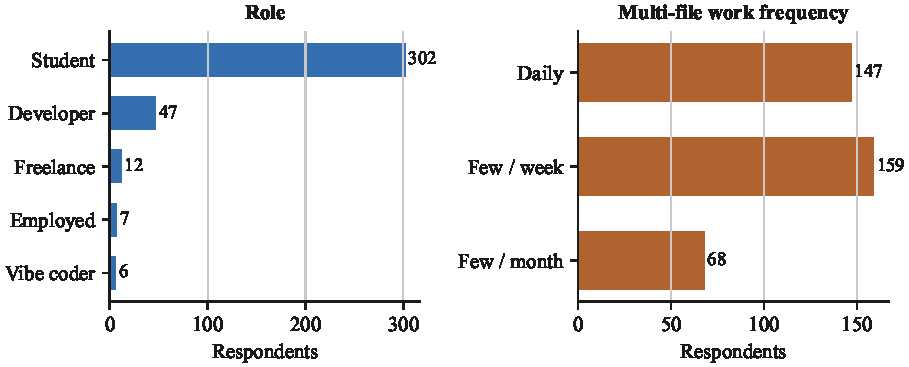
\includegraphics[width=\textwidth]{Figures/fig_profile.pdf}
    \caption{Respondent role and work frequency.}
    \label{fig:profile}
\end{figure}

The sample is skewed towards students, which fits the target early-adopter profile, and multi-file work is common in all groups.

ARTEMIS is a desktop assistant within this domain, which works on explicitly granted folders. It reinstates context following an interruption by reporting on what was last active and what was to be done next. It organises files by proposing a set of moves the user previews and approves. It collects content of multiple documents into a synthesis where each assertion is accompanied by a reference to its source. It monitors repetitive manual steps and provides, on the third repetition, to automate them. It reads source code to describe errors and suggests fixes as a difference the user reviews. It browses the web on request, prepares electronic mail to be approved and drafts documents as new files. All these can be accessed both through voice and typing.

All this is bounded by the system. It cannot solve a path not within a given workspace, it does not have a command that removes user data, and all operations that modify a file or exit the machine are subject to approval by the user.

\section{Problem Statement}
Multi-file knowledge workers lose a lot of time and effort in restoring context after interruptions and in doing routine file and correspondence tasks, and the artificial intelligence assistants that can alleviate this burden require wide, unrestricted access to the machine of the user, exposing them to privacy risks, and risking unintended modification and loss of user control that many users are not ready to accept.

\section{Problem Elaboration}
The issue is divided into five sub-problems, and each of them is addressed by the project in a different manner.

The former is loss of context following interruption. When a user comes back to work after a day or more of a break, the information required to restart is spread across the filesystem, the applications that were open, and the memory of the user, and the latter is the part that breaks. In our questionnaire, we discovered that 44 percent of the people always or frequently have trouble remembering what they were doing when they revisit a project, and only 7 percent never. This distribution is depicted in Figure~\ref{fig:return}.


The figure indicates the frequency of returning to a project after a day or more and failing to remember what they were doing or what to do next.


The second is file disorder accumulation. Organisation decays constantly and is only repaired periodically, so the filesystem is constantly drifting out of any form that would allow material to be easily located. Of our respondents, 59 percent said they found their folders getting messy more quickly than they could clean them by hand, with an average of 3.6 out of five..

\begin{figure}[H]
    \centering
    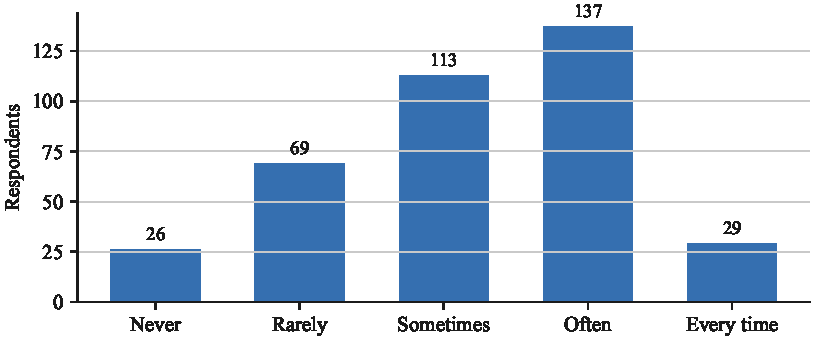
\includegraphics[width=0.82\textwidth]{Figures/fig_return_struggle.pdf}
    \caption{Difficulty resuming work after a break.}
    \label{fig:return}
\end{figure}

The third is the cost of routine manual work, which is individually small and collectively significant. Respondents estimated the total weekly time lost to reorientation, tidying, repeated manual tasks and searching scattered notes, and 42 percent placed it above an hour a week with 14 percent above three hours. Figure~\ref{fig:time} shows the distribution, whose mode falls between thirty and sixty minutes. This is steady friction rather than crisis, which is the correct way to understand what the system is relieving.

\begin{figure}[H]
    \centering
    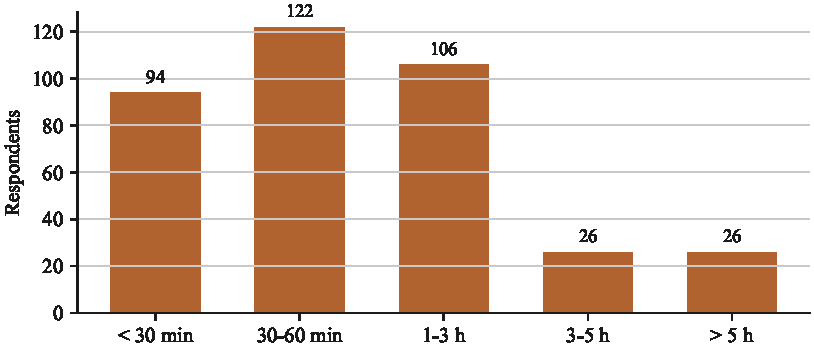
\includegraphics[width=0.82\textwidth]{Figures/fig_time_lost.pdf}
    \caption{Estimated time lost per week.}
    \label{fig:time}
\end{figure}

The estimate covers reorienting after breaks, tidying files, repeating manual tasks and searching scattered notes.

The fourth is that this work remains unautomated for reasons of trust and knowledge rather than absence of need. When asked why they had not already automated these tasks, 36 percent of respondents cited not trusting automation to do it correctly and 28 percent cited not knowing how, as shown in Figure~\ref{fig:whynot}. The tasks exist and are recognised; what is missing is an instrument the user is willing to point at them.

\begin{figure}[H]
    \centering
    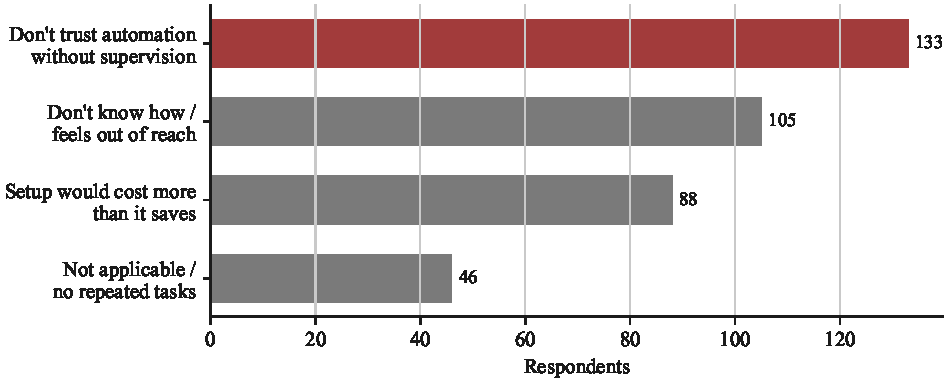
\includegraphics[width=0.82\textwidth]{Figures/fig_why_not_automated.pdf}
    \caption{Reasons for not automating repeated manual tasks.}
    \label{fig:whynot}
\end{figure}

Distrust of automation and lack of know-how dominate.

The fifth is the access bargain that existing assistants impose, which is the sub-problem that distinguishes this project. A capable assistant is generally granted wide access to the machine, and the user is then unable to determine what it holds, what it may do, or how to reverse what it has done. Our questionnaire tested the alternative directly and found that 65 percent of respondents rate an assistant confined to explicitly added files as meaningfully more trustworthy than one with full access, with a mean of 3.8 on a five-point scale.

\section{Goals and Objectives}
The goal of the project is to demonstrate that a bounded, opt-in assistant can deliver useful multi-step automation while measurably improving user trust and preserving user control.

The objectives that realise this goal are as follows.

\begin{itemize}
    \item To create a desktop helper that only works within folders that the user has granted access to, so that access beyond a grant is structurally impossible and not just forbidden.
    \item To minimize the time and effort users take to resume interrupted work and to carry out routine file, document and correspondence activities.
    \item To ensure that the user is in control of all the consequential actions by passing it through preview, approval and undo.
    \item To ensure that the system does not destroy any user data, by giving no code path to a destructive operation.
    \item To render visible and individually removable by a disclosure panel everything the system contains.
    \item To advocate voice as a full interaction mode that is subject to the same approval gates as typing.
    \item To test the system in terms of time to complete a task, cognitive workload, usability and trust, and to report inherited limitations in an honest manner.
\end{itemize}

\section{Project Scope}
This project is to design, construct and test a desktop assistant to assist one user in managing daily work in clearly defined workspaces. The system will enable the user to:

\begin{itemize}
    \item Assign a folder as a working directory, and unassign it to delete all the descendants
    \item Resume interrupted work by looking at what was last active and what was to be done next.
    \item Clean up a folder by viewing and accepting a suggested set of moves.
    \item Synthesise notes in multiple documents with each claim traceable to its origin.
    \item Get an offer to automate a manual sequence once it has been repeated three times.
    \item Ask questions about source code and receive explanations and proposed fixes as differences
    \item Search the web on demand
    \item Draft electronic mail and send it only after approving the draft
    \item Always written as new files, draft documents.
    \item Perform any of the above by voice as well as by typing
    \item Check all that the system contains, and erase any of it.
    \item Undo a plan that has been approved as a unit.
\end{itemize}

The system will be implemented in Python. Multi-step plans will be produced using LangGraph~\cite{ref:langgraph}, which provides an explicit pause point before any workspace-changing or outward call. Language model access will be local-first through Ollama~\cite{ref:ollama}, with an optional and per-workspace cloud fallback. Persistence will use local SQLite~\cite{ref:sqlite} together with a per-workspace vector index. The interface will comprise a command line surface and a local graphical control panel.

The project deliverables will be:

\begin{itemize}
    \item A working desktop assistant implementing the features above
    \item This design and specification document, and the evaluation report that follows.
    \item A user manual
    \item A test suite of the boundary, policy, approval and undo guarantees.
\end{itemize}

The project scope does not include the following:

\begin{itemize}
    \item Any access to any part of the filesystem not within a granted workspace.
    \item Deletion or unsnapshotted overwriting of user data.
    \item Autonomous action, i.e. any file change or external action performed without authorization.
    \item Background browsing, screen recording, keystroke capture or always-on audio recording
    \item Mobile applications, in addition to the optional remote control surface in Chapter 6.
    \item Multi-user, shared or enterprise deployment
    \item Storing user information on any server of the project.
\end{itemize}

\section{Sustainable Development Goal (SDG)}
The project is aimed at Sustainable Development Goal 9, Industry, Innovation and Infrastructure, and specifically at 9.5, which is related to the improvement of scientific research and the modernization of technological capacities~\cite{ref:sdg}. The complete list of goals is shown in Figure~\ref{fig:sdg}.

The local-first design of the project is its contribution to this goal. The default configuration of the system does its job with a model that runs on the personal machine of the user, so the functionality it offers is not contingent on constant connectivity to a data centre, on a subscription, or on whether the user is willing to send personal documents to a third party. This is important to the population that the project is aimed at. Independent practitioners and students, especially in areas with patchy or expensive connectivity, are exactly the users where a cloud-dependent assistant is least available, and a local-first assistant brings an existing technological feature to them at a cost they can afford. Our data confirms the choice: local-first operation was the most popular deployment option among respondents at 40 percent, compared to 22 percent who actively favored cloud.

The project also supports Goal 8, Decent Work and Economic Growth, target 8.2 on productivity through technological upgrading, as the aim of the system is to eliminate repetitive friction in knowledge work and reallocate that time to productive work.

\begin{figure} [!h]
    \centering

\includegraphics[width=0.8\textwidth]{Figures/Picture1}
    \caption{The seventeen UN Sustainable Development Goals.}
    \label{fig:sdg}
\end{figure}

The goals are represented in the figure as numbered coloured tiles, each consisting of the goal number, its short title and a representative icon. The project is aimed at Goal 9, Industry, Innovation and Infrastructure, and secondarily Goal 8, Decent Work and Economic Growth.

The objectives that this project will respond to are presented clearly in Figure~\ref{fig:sdgsel}: SDG 9, Industry, Innovation an.d Infrastructure (target 9.5) as the primary goal, and SDG 8, Decent Work and Economic Growth

\begin{figure}[H]
\centering
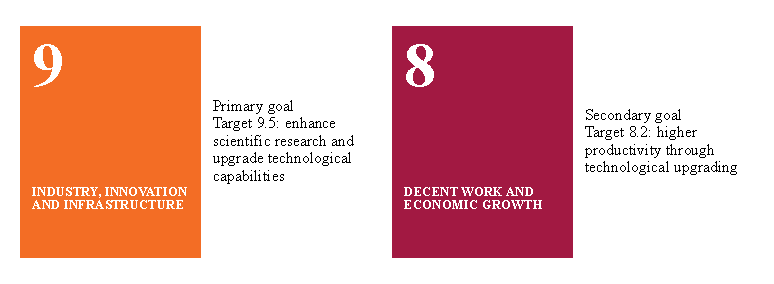
\includegraphics[width=0.9\textwidth]{Figures/fig_sdg_selected.pdf}
\caption{SDGs targeted by this project.}
\label{fig:sdgsel}
\end{figure}

\section{Constraints}
The project operates under the following constraints, each of which shapes the design presented in Chapter 6.

\begin{itemize}
    \item The system should be able to execute on a standard student laptop, which limits the size of the local language model, the resident memory footprint and the size of the acceptable index.
    \item The core operation should not need to be connected to the internet, and thus any feature that relies on the network should not fail but instead be limited to a specified threshold.
    \item The user data should not exit the machine unless there is an explicit per-workspace opt-in, which puts the egress decision in the model router instead of in any feature.
    \item The system should not have any inbound listening port outside the loopback interface, and thus the optional remote plane should not accept connections but should dial out.
    \item The credentials should be stored in the operating system keyring and should never be on disk in the system own storage tree.
    \item The team of three has to finish the project in two academic semesters, which means that the most risky parts should be constructed and tested as soon as possible.
    \item The analysis should be performed using the participants who are selected based on the networks of one institution, which limits the external validity of its findings.
\end{itemize}

\section{Business Opportunity}
The assistant market currently exists as a split between tools that can but require wide access and tools that can but require step-by-step guidance. The gap between them is the opportunity that this project will fill, and our data shows that the gap is not filled by a hypothetical preference: most respondents found a limited assistant more credible, and the most frequent reason they gave as to why they had not automated this work yet was distrust of automation.

Three conditions make the opportunity actionable. Local language models are now sufficiently powerful to execute useful inference on consumer hardware, and local-first operation is no longer aspirational but practical. The regulatory and personal sensitivity to data processing is on the increase, and it adds to the worth of an assistant that can say exactly what it contains. The target population is already familiar with assistants, since 77 percent of our respondents have used one, so the product does not have to establish the category.

The risk that corresponds is differentiation, and our data reveals it clearly. One of the common themes in free-text answers was that the idea seemed to be already addressed by the existing developer assistants. The solution is the bounded workspace and local-first operation, and the discovery is that this should be explicitly written in the product and not left to the user to deduce.

\section{Stakeholders Description/ User Characteristics}
The users of this system are those who do knowledge work on their own machines, along with the roles of evaluating and maintaining the project..

\subsection{Stakeholders Summary}
Table~\ref{tab:stakeholders} identifies each stakeholder, their role with respect to the system, and their principal concern. Table 2.1: Stakeholders and their concerns.

{\Needspace*{7\baselineskip}
\begin{longtable}{|p{3.2cm}|p{5.0cm}|p{5.6cm}|}
\caption{Stakeholders and their concerns.}\label{tab:stakeholders}\\*
\hline
\textbf{Stakeholder} & \textbf{Role} & \textbf{Primary concern} \\*
\hline
\endfirsthead
\caption[]{continued from previous page}\\*
\hline
\textbf{Stakeholder} & \textbf{Role} & \textbf{Primary concern} \\*
\hline
\endhead
\hline
Student & Primary user. Works across documents, notes and source files on a personal laptop, frequently interrupted. Represents 81 percent of the research sample. & Recovering context quickly; keeping personal and academic files private; no configuration burden. \\
\hline
Developer & Primary user. Works across source files and documentation, and is the principal user of the code assistant. Represents 13 percent of the sample. & Correctness of proposed changes; never having code modified without review. \\
\hline
Freelancer or knowledge worker & Primary user. Manages client documents and correspondence. & Confidentiality of client material; reliable correspondence drafting with approval. \\
\hline
Project supervisor & Assesses the project's academic soundness and progress. & Traceability of design decisions to evidence; feasibility within the timeline. \\
\hline
Evaluation panel & Assesses the delivered project against its stated objectives. & Whether the hypothesis was tested and whether limitations are stated honestly. \\
\hline
Development team & Designs, implements and evaluates the system. & Preserving the architectural invariants under change; completing the scope in time. \\
\hline
Future maintainer & Extends the system after the project concludes. & Locating the enforcement points; understanding which properties must not be broken. \\
\hline
\end{longtable}
}

\subsection{Key High-Level Goals and Problems of Stakeholders}
The primary users share a single high-level goal, which is to spend less time on the mechanics of their work and more on its substance, and they share a single high-level problem, which is that the tools capable of granting this require a degree of access they are not prepared to give. Our research refines this general statement in four respects that bear directly on the design.

Users are divided on how much they wish to be asked. The questionnaire presented a choice between an assistant that seeks approval before every file change or outward action and one that acts on reasonable requests and permits review and undo afterwards. The split was 192 to 182, shown in Figure~\ref{fig:pref}. No single interaction model satisfies this population, and approval granularity is therefore specified as a user-configurable setting in Chapter 4 rather than fixed in the design.

\begin{figure}[H]
    \centering
    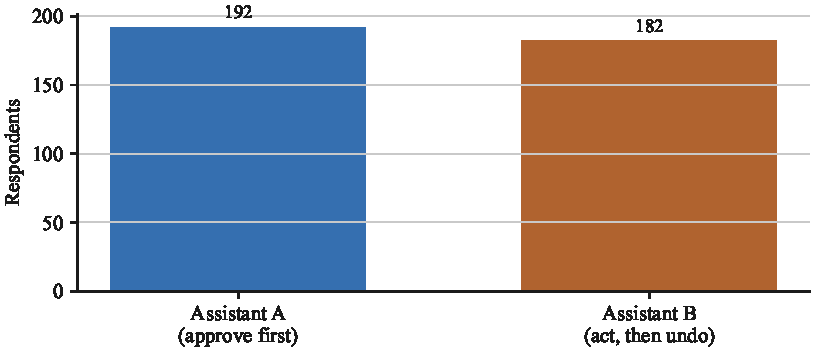
\includegraphics[width=0.72\textwidth]{Figures/fig_assistant_pref.pdf}
    \caption{Approval-first versus act-then-undo.}
    \label{fig:pref}
\end{figure}

The population is close to evenly divided.

Users will tolerate a mistake if they can reverse it. Asked what a single wrong or unwanted suggestion would make to their usage, 65 percent would still use the system, some more cautiously, and only 10 percent would give up. This observation confirms that a visible and reliable undo is more useful than an unattainable perfection, and it is why the undo journal is defined as a necessity and not a luxury.

Users will stop for reasons of fit rather than friction. The most common reasons that were predicted to abandon the system after a week were that it did not fit existing habits, at 27 percent, and that it made a mistake that the user could not trust it to avoid in the future, at 24 percent. Approval fatigue was the smallest named risk at 10 percent. This moderates an instinct of natural design: minimizing the number of prompts would be the least frequent worry, and would undermine the trust that the approval model offers.

Users desire the system to know their structure, and this is a request that the bounded design must consider keenly. The most requested feature that was not already planned was that the assistant should learn how the user organises their folders over time. This is defined as per-workspace memory, which can be seen and deleted in the disclosure panel, such that personalisation does not expand the bounded-scope guarantee silently.


\section{Conclusion}
The vision of the project has been mentioned in this chapter. It defined a two-half problem, the expense of restarting interrupted work and the reluctance of many users to grant an assistant wide access, and it framed the work by objectives, a scope, exclusions and constraints. It determined the sustainable development goal that the project is supporting, the opportunity that it is addressing and the stakeholders whose characteristics dictate the design. All this is supported by the underlying research, the distributions of which are provided in Appendix A. The next chapter is a review of the literature against which these claims are tested.

\chapter{Literature Review / Related Work}
This chapter is a review of the research literature and the applications that are available in the project. The review discusses 26 studies that are grouped into seven themes, each of which is a capability or a guarantee that the system should offer. For each theme the chapter summarises the work, analyses its strengths and weaknesses, and states the relationship to the proposed system. The chapter ends by determining where the project actually seals a gap, where it seals a gap in part, and where it inherits a limitation it cannot boast of having addressed.

\section{Definitions, Acronyms, and Abbreviations}
The terms listed below are used in this chapter specifically, in addition to those defined in Chapter 1.

\textbf{Agentic system}: a system in which a language model plans a sequence of steps and invokes tools to carry them out, rather than only producing text\\
\textbf{Human-in-the-loop}: an arrangement in which a person approves or corrects a system's proposed action before it takes effect\\
\textbf{Prompt injection}: an attack in which instructions embedded in retrieved content are treated by a model as commands from the user\\
\textbf{Hallucination}: generated content that is not supported by the source material it purports to summarise\\
\textbf{Attribution}: the property that a generated statement is genuinely supported by the source it cites\\
\textbf{Faithfulness}: the consistency of a generated summary with the document it summarises\\
\textbf{Approval fatigue}: the decline in scrutiny that occurs when a user is asked to approve actions frequently\\
Approval fatigue: the reduction in scrutiny that arises when a user is requested to approve actions is an architectural defence that isolates a trusted component against untrusted data or code.

\section{Detailed Literature Review}
The review is organised into seven themes. Themes one, two, and three are about the core behaviour of the system, which includes task resumption, limited agents and trust, and agentic planning. Themes four and five relate to two capabilities, voice interaction and code assistance. Themes six and seven are about the accuracy of generated text, including hallucination and citation accuracy.

\subsection{Task Interruption and Resumption}
This problem is started with an observational finding. An office study of normal computer use has determined that when individuals are interrupted in a task, on-screen indicators like an open window instead of minimised are what allow them to re-engage in the task later~\cite{ref:iqbal2007}. The experiment was carried out in actual working conditions, not in a laboratory, and it was terminated at diagnosis: no system was suggested to the case where it is no longer convenient to leave a window open, e.g. after a restart or a few days break.

This diagnosis was later transformed into a tool. ScreenTrack captures a background time-lapse of the screen and lets a user scroll through it visually to find and reopen something they recall seeing, based on the idea that people remember sequences of visual scenes better than file names or timestamps~\cite{ref:hu2020}. In a controlled laboratory experiment it fared well with recent and visually distinct activity.

The weaknesses and strengths of this pair are complementary. The strength of the field study is the ecological validity and the weakness is that it did not generate any intervention. The strength of ScreenTrack is that it operationalises the finding, and its weaknesses were admitted frankly by its authors: retrieval is slower with a longer history, the method relies on tasks being visually distinguishable and thus is not well suited to textheavy work, and it was not tested in long-term multi- application use. Another apparent conflict is between a continuous screen recording and the privacy expectations of the users that this project is aimed at.

The connection to the proposed work is not an extension but a deliberate divergence. The resumption feature specified in this report does not record the screen at all. It works based on the file index and on notes that the user has written, matching on file name, recency and explicit text, and is therefore not dependent on whether two screens are similar to each other. Since a workspace is delimited by construction, the issue of searching a long history is also avoided, as there is only a short list of recent and relevant items to display. The truthful qualification is that the resumption benefit is a design claim and not a demonstrated claim because the system has not been field-validated in the same way as the original study.

\subsection{Bounded Artificial Intelligence Agents and Trust}
Another body of literature poses the question of how the autonomy of an agent can be limited to boundaries that a person can rely on. One is developer-facing. A trace-based assurance system records all actions of an agent as a structured trace with machine-checkable contracts attached to each step, such that a failure can be traced to a precise point and re-executed deterministically, mediating each action as allow, rewrite or block based on per-agent capability constraints~\cite{ref:paduraru2026}.

A recent security survey looks at the same space through the lens of systems that require human sign- off~\cite{ref:kim2026}. It examines privilege separation as an architectural defence, and compares it to the separation that an operating system provides between a trusted kernel and untrusted programs, and extends this to the isolation of a planning component against untrusted external data. It then looks at the constraints of human-inthe-loop approval itself, and its conclusion is not favourable: frequent approval prompts cause decision fatigue that negates the safety benefit they are designed to offer, and most users do not have the background to evaluate what they are being asked to approve, so they either approve risky actions without actually evaluating them, or they reject harmless ones. This is an open problem that the survey does not provide a solution to.

The advantage of this body of work is that the machinery to bound an agent is already in place and is well known. Its drawback, as it currently stands, is that it is designed to support organisations that have security personnel and infrastructure as opposed to an individual operating an assistant on their own computer. Another interesting feature of the assurance framework is that it lacks a way to reverse an action after it has been executed.

The connection to the proposed work is two-way. The workspace model of this project is a plain- language implementation of the same concepts: a folder that the user chooses instead of a sandbox that an administrator describes, and a readable preview instead of a machine-checked contract. Opposite the assurance framework the project contributes exactly what the assurance framework lacks, which is reversal after the fact, and this is one of the most direct correspondences in the review. Against the security survey the project must yield a point instead of asserting one. It does not address approval fatigue. It is based on the same mechanism that the survey finds unresolved, and there is nothing in the current design that differentiates between a routine approval and a risky one or minimizes prompts as trust is built. This is a limitation that is inherited by adopting this method in the first place, and the analysis should test it explicitly, not suppose that the constrained workspace will eliminate it.

\subsection{Agentic Reasoning, Planning and Undo}
A large literature has shifted language models out of text generation and into goal-oriented reasoning, step planning and action. Reflexion enables an agent to assess its own past efforts, compose verbal reflections and store them as episodic memory to enhance subsequent efforts without retraining, enhance performance on decision-making, reasoning and coding tasks~\cite{ref:shinn2023}. Toolformer is more focused, training a model to invoke an external tool like a calculator or a search engine in a more or less self- supervised way when and how~\cite{ref:schick2023}. Generative Agents builds upon the memory-and-reflection concept by showing that a population of agents can act in a coherent way across simulated days by storing, retrieving and reflecting on experience, as well as reporting failures such as false retrieval and falsified memory detail~\cite{ref:park2023}. ReAct combines reasoning, acting and observing in one loop and demonstrates that the combination is more effective in performance and interpretability, and is susceptible to repetitive loops of action and ineffective recovery in case an action yields an unhelpful result~\cite{ref:yao2023react}. Tree of Thoughts allows a model to explore many lines of reasoning and retrace unpromising ones, generating large payoffs on puzzle-like problems at a real computational cost~\cite{ref:yao2023tot}.

The strength of this literature is that it establishes reasoning, tool use and reflective memory as a workable substrate for agent behaviour. The common weakness of all of them is the environment in which each system is tested: Reflexion on its own history of attempts, Toolformer on single tool calls it cannot easily compose, Generative Agents in a sandbox world, and ReAct and Tree of Thoughts on benchmark tasks. None of them has a confined workspace of a real user in the context of normal interrupted work, and none of them needs the sort of approval that would make consequential actions reversible.

The proposed work lies in that gap. It takes the underlying combination of reasoning, tool use and memory but applies it to the actual files, notes and stated intentions of a user instead of the history of the agent or a simulated environment, and it encases the resulting multi-step plans in preview, approval and undo, which none of these systems offer. The failure modes this literature reports are also a direct warning. Artificial memory and recursive reasoning loops characterize exactly the fallacies that the resumption and synthesis capabilities should protect against, and they suggest that the number of unsupervised steps between user checkpoints should be small instead of believing that a longer autonomous chain is safe.

\subsection{Voice Interaction Parity}
This theme is whether individuals can perform practical computer tasks as well by voice as by typing, and how voice interaction is to be assessed. The state of the field is determined by two systematic reviews. The former performs a bibliometric review of user experience with voice interfaces and suggests a six-category classification of research, including voice-related variables such as gender, accent, personality and style~\cite{ref:deshmukh2024}. The second compares voice assistant usability to the ISO 9241-11 model of effectiveness, efficiency and satisfaction~\cite{ref:dutsinma2022}.

There are three empirical studies that provide tangible design advice. One shows that speech has a realtime indication of user experience that post-hoc questionnaires fail to measure, and pause duration and disfluency rate are additional measures~\cite{ref:ma2026}. Another looks at verbal cues in waiting times, discovering that a long wait is best managed by an indicator that not only tells what is going on but also adds a touch of humour, but a short wait can be managed by an indicator alone and no more~\cite{ref:zhang2025}. A third deals with the delay in response when talking to virtual agents in free-form conversation, where natural conversational fillers are better than artificial tones~\cite{ref:wang2025}.

The advantage of this literature is that it provides usable thresholds and design guidelines, such as a foursecond latency target. Its limitation, as both reviews mention, is that voice usability is researched in bits and that conventional usability measures do not consider voice-related issues like trust and cognitive load.

The connection to the proposed work is two-fold. In design, the waiting-indicator and filler results dictate the behavior of the voice mode during the production of a plan, which should be a spoken explanatory indicator, not silence or a generic tone. To assess, the fact that the literature agrees that voice as a full interaction mode compared to practical multi-step tasks is under-researched is the contribution: this project will compare voice to typing in terms of ease of use, task time, cognitive workload and trust. The speech-analysis method is a non-design feature that is an optional addition to that assessment.

\subsection{Code Assistance with Human Review}
There are five studies that discuss the circumstances in which language model assistance with code is helpful. HULA illustrates a plan, generate and human-approve loop in a real deployment, reporting an 82 percent plan approval rate and discovering that the quality of output is strongly dependent on the quality of the input context~\cite{ref:takerngsaksiri2025}. HiLDe is more granular, driving generation token by token, and reports two warnings: regeneration may silently overwrite previous user edits, and showing too many options overwhelms users~\cite{ref:gonzalez2025}. An analysis of suggestion timing looks at when an inline assistant ought to show a suggestion and cautions against maximising the acceptance rate at the cost of usefulness~\cite{ref:mozannar2024}. A taxonomy of expert steering strategies recognizes the actions through which an individual redirects a model, such as pointing out a particular error, explaining a requirement and re-orienting the strategy, and observing that certain strategies assume expert knowledge~\cite{ref:chidambaram2024}. Lastly, a review of language models as code reviewers identifies systematic overcorrection, where models generate requirements and label correct code as incorrect, and that longer explanations are worse than shorter ones~\cite{ref:jin2026}.

The advantage of this literature is that it confirms the human-approval loop as a successful interaction model and not a fallback. Its general infirmity, which the overcorrection study says is most acute, is that model judgement concerning code is helpful but not reliable in itself, and that explanations do not render it more reliable.

The relationship to the proposed work is direct. The code assistant mentioned in this report takes the form of HULA but is scaled down: it displays the source of the workspace, answers questions, describes errors and suggests a fix as a difference that the user can accept, and does not open pull requests or operate within a repository. The warnings of HiLDe are converted into two design principles, namely to introduce a single proposed change at a time and never to change code that the user has not accepted. Since the assistant is not invoked continuously but instead provides suggestions on demand, the suggestion-timing issue does not occur, which is a conscious benefit of the on-demand model. The overcorrection result is the immediate reason why a change should never be applied automatically, and the mitigation is the difference-plus-approval design, which alleviates but does not eliminate the underlying limitation.

\subsection{Hallucination in Artificial Intelligence Summarisation}
Four studies follow this issue up to diagnosis to meta-evaluation. The former proved that the content of hallucinations was present in all abstractive summarisation systems that were tested, and entailment between source and output was the correct check~\cite{ref:maynez2020}. FactCC was then succeeded by a lightweight, trainable consistency checker, the nearest thing in the literature to a component that might be directly adopted~\cite{ref:kryscinski2020}. FRANK then benchmarked the available factuality metrics and discovered that none of the metrics identifies all types of errors~\cite{ref:pagnoni2021}. SummEdits generalized the question to frontier models and discovered that even the most robust models rate faithfulness poorly~\cite{ref:laban2023}.

The merit of this literature is that its conclusion is consistent over a decade: hallucination is widespread, standard measures of overlap fail to identify it, no single measure is consistently reliable, and models are poor predictors of their own accuracy. Its engineering weakness is that it provides no full solution, just partial detectors and the suggestion to integrate them.

The connection to the proposed work should be expressed as a gap and not a solution. The synthesis feature works on a small, user-selected set of documents, a more limited and controlled task than open-domain summarisation and thus offers a smaller surface on which to hallucinate. It does not kill it. The existing design has no faithfulness check, and thus this is an open gap and not something that the bounded workspace solves. The specified direction is an entailment-style or FactCCstyle check post-generation, with the user kept in the loop, and the SummEdits finding rule eliminates the tempting shortcut of requesting the model to check its own citations.

\subsection{Retrieval-Augmented Generation Citation Accuracy}
Three articles discuss the question of whether generated text actually substantiates the sources it refers to. The former provides a practical definition of attribution, which is presented in the form of whether a statement passes the test that the statement is true according to the source cited~\cite{ref:rashkin2023}. ALCE subsequently benchmarked the capability of models to produce text with citations and incomplete citation was prevalent~\cite{ref:gao2023}. A review of implemented generative search engines revealed that approximately a quarter of citations failed and approximately half of sentences were not completely supported~\cite{ref:liu2023}.

The merit of this literature is that it provides a standard and empirical evidence of the extent to which real systems are below it. Its drawback is that it offers a measuring device and not a policing tool.

The relationship to the proposed work is partial. The synthesis option eliminates the retrieval component of the problem by pre-selecting the documents by the user, and the citation map in Chapter 6 brings each chunk back to its file and line. What the existing design fails to do is to ensure that a citation is provided to support the claim that is attached to it, or that all claims have one. The correct calibration in this case is the audit of deployed products: even mature products with specific citation engineering fail these tests at significant rates, and this is a reason to consider citation verification as a necessary task and not to believe that citing out of a small known set is safe by default.

\subsection{Related Development Projects and Applications}
In addition to the research literature, there are three families of existing application that are relevant to the project. The inline coding assistants built into development environments offer continuous suggestion in a single editor, and their advantage is immediacy and their disadvantage is that they only deal with code and work with whatever the editor can access. Multi-step plans are run by agentic command-line assistants on the machine of a developer, and their power is real multi-step capability and their weakness is the scope of access they need and the difficulty of undoing what they have done. General-purpose conversational assistants are generally capable but have no long-term, structured connection to the filesystem of the user, so they cannot resume work or act on files unless material is provided to them each time.

Our own study shows that this landscape is not just a question of technical comparison but of positioning. One of the common themes in free-text answers was that the proposed system seemed to be already addressed by the existing developer assistants, which confirms that differentiation should be made a point of argument. The distinguishing properties are the enforced workspace boundary, default local-first operation, the structural unavailability of destructive operations, and the disclosure panel that causes the trust claim to be falsifiable and not merely persuasive..

\section{Literature Review Summary Table}
Table~\ref{tab:lr} summarises the reviewed studies, identifying the theme each addresses, the contribution it makes, its relevance to this project and its limitations.

{\small
\Needspace*{3\baselineskip}
\begin{longtable}{|p{2.6cm}|p{2.0cm}|p{3.6cm}|p{4.6cm}|}
\caption{Summary of the reviewed literature.}\label{tab:lr}\\*
\hline
\textbf{Study} & \textbf{Theme} & \textbf{Relevance to this project} & \textbf{Limitations} \\*
\hline
\endfirsthead
\caption[]{continued from previous page}\\*
\hline
\textbf{Study} & \textbf{Theme} & \textbf{Relevance to this project} & \textbf{Limitations} \\*
\hline
\endhead
\hline
Iqbal and Horvitz \cite{ref:iqbal2007} & Resumption & Establishes that resumption depends on persistent cues, motivating the session resume feature & Diagnosis only; proposes no system; cues fail after restart or a multi-day gap \\*
\hline
Hu and Lee \cite{ref:hu2020} & Resumption & Demonstrates a resumption tool, whose weaknesses this project avoids structurally & Slow retrieval over long histories; requires visually distinct tasks; privacy cost of screen recording \\*
\hline
Paduraru et al. \cite{ref:paduraru2026} & Bounded agents & Contract mediation and capability limits inform the policy engine & Built for organisations with security staff; no mechanism to undo an executed action \\
\hline
Kim et al. \cite{ref:kim2026} & Bounded agents & Privilege separation informs the planner and dispatcher split; documents approval fatigue & Names approval fatigue as an open problem without offering a solution \\
\hline
Shinn et al. \cite{ref:shinn2023} & Agentic planning & Episodic written memory as a substrate for agent behaviour & Evaluated on the agent's own past attempts, not on real user work \\
\hline
Schick et al. \cite{ref:schick2023} & Agentic planning & Self-supervised tool invocation informs the tool contract & Isolated tool calls that cannot readily be chained into plans \\
\hline
Park et al. \cite{ref:park2023} & Agentic planning & Memory, retrieval and reflection architecture informs the memory design & Sandbox world; reports fabricated memory and incorrect retrieval \\
\hline
Yao et al. \cite{ref:yao2023react} & Agentic planning & Interleaved reasoning and acting informs the bounded reflection loop & Repetitive action loops; poor recovery from unhelpful observations \\
\hline
Yao et al. \cite{ref:yao2023tot} & Agentic planning & Search over reasoning paths informs the cycle cap on planning & Substantial computational cost; benchmark tasks only \\
\hline
Deshmukh and Chalmeta \cite{ref:deshmukh2024} & Voice & Classification of voice user experience research informs evaluation measures & Voice usability studied in fragments; no unified framework \\
\hline
Dutsinma et al. \cite{ref:dutsinma2022} & Voice & ISO 9241-11 framing of usability informs the evaluation instrument & Standard metrics omit trust and cognitive load \\
\hline
Ma et al. \cite{ref:ma2026} & Voice & Speech as a real-time experience signal; optional evaluation enhancement & Requires turn-by-turn audio capture, which this project does not plan \\
\hline
Zhang et al. \cite{ref:zhang2025} & Voice & Waiting-indicator design for periods while a plan is produced & Findings specific to the wait durations tested \\
\hline
Wang et al. \cite{ref:wang2025} & Voice & Natural fillers preferred over tones during response delay & Studied in free-form conversation rather than task execution \\
\hline
Takerngsaksiri et al. \cite{ref:takerngsaksiri2025} & Code assistance & Validates the plan, generate and approve loop at 82 percent plan approval & Output quality heavily dependent on supplied context \\
\hline
Anaya Gonzalez et al. \cite{ref:gonzalez2025} & Code assistance & Cautions against silent overwriting and excessive alternatives & Token-level granularity finer than this project requires \\
\hline
Mozannar et al. \cite{ref:mozannar2024} & Code assistance & Establishes that on-demand invocation avoids the suggestion-timing problem & Applies to inline assistants; acceptance rate is a misleading objective \\
\hline
Chidambaram et al. \cite{ref:chidambaram2024} & Code assistance & Steering taxonomy informs follow-up prompts when a fix is rejected & Some strategies presuppose expert knowledge \\
\hline
Jin and Chen \cite{ref:jin2026} & Code assistance & Direct justification for never applying a code change automatically & Models overcorrect; longer explanations worsen reliability \\
\hline
Maynez et al. \cite{ref:maynez2020} & Hallucination & Entailment identified as the appropriate faithfulness check & Hallucination present in every system tested; no complete remedy \\
\hline
Kryscinski et al. \cite{ref:kryscinski2020} & Hallucination & FactCC is the most directly adoptable consistency checker & Not currently used by this project; a stated open gap \\
\hline
Pagnoni et al. \cite{ref:pagnoni2021} & Hallucination & Warns against relying on a single faithfulness metric & No single metric detects every error category \\
\hline
Laban et al. \cite{ref:laban2023} & Hallucination & Rules out self-checking of citations by the model & Even frontier models judge faithfulness poorly \\
\hline
Rashkin et al. \cite{ref:rashkin2023} & Citation & Supplies the attribution standard for synthesis output & A standard rather than an enforcement mechanism \\
\hline
Gao et al. \cite{ref:gao2023} & Citation & Benchmarks citation generation; motivates completeness checks & Incomplete citation common even in purpose-built systems \\
\hline
Liu et al. \cite{ref:liu2023} & Citation & Calibrates expectations against deployed products & A quarter of citations unsupported; half of sentences not fully supported \\
\hline
\end{longtable}
}

The table gives the theme, contribution, relevance to this project and stated limitations of each study.

\section{Conclusion}
The reviewed literature establishes three conclusions for this project.

The project addresses a real gap in four aspects. It uses multi-step agentic planning on a limited, user- selected desktop workspace instead of a simulated world, a single task or an open repository, a combination that the planning literature leaves open. It exposes agent memory and allows it to be edited by the user via the disclosure panel, where the reviewed systems execute memory as an opaque background process and report fabricated and mis-retrieved entries. It offers reversal following a previewed action, which the assurance framework does not have at all. It assesses voice as a holistic interaction mode compared to practical multi-step tasks, which both voice reviews recognize as under- explored.

The project partially addresses three other gaps. Its limited capability scoping is a plain-language implementation of the capability limits and privilege separation the security literature talks about, sacrificing rigour to usability. Its resumption feature operationalises an established finding without having replicated the field validation of that study. Its code assistance uses a proven human-approval loop but is still susceptible to the errors of the underlying model, which approval reduces but does not eliminate.

The project has three limitations that it does not address, and they are mentioned here instead of being postponed. It fails to address approval fatigue, which the security survey records as an open issue in precisely the mechanism that this design relies on, and the test must evaluate it across multiple sessions. It has no faithfulness check on synthesised text, thus the narrower task minimises but does not remove the exposure the summarisation literature records. It does not confirm that their claims are supported by citations or that all claims have a citation, which the citation literature demonstrates to be unreliable even in deployed products of high quality.

These findings inform the requirements in Chapter 4 and the design in Chapter 6, and they establish the conditions under which the evaluation in the second phase of the project should report its findings.


\chapter{Software Requirement Specifications}
This chapter specifies the requirements for the system. It enumerates the features, specifies the functional requirements and their users, enumerates the quality attributes and non-functional requirements, documents the assumptions on which the specification is based, outlines the principal use cases, outlines the hardware and software requirements, describes the interface and the database design, and discusses the risks. Every requirement is formulated in a verifiable manner, such that a completed implementation can be verified against it instead of being evaluated informally.

The requirements are named with a prefix and a number. Functional requirements are denoted as FR- 1 and non-functional requirements as NFR-1 and quality attributes as QA-1.

\section{List of Features}
The system offers the following features, in the sequence in which they are constructed. The order is based on measured demand, which is reported in Chapter 3, and technical risk, such that the elements on which all other features rely are built and tested first..

\begin{itemize}
    \item The workspace management, where a user gives a folder, checks what the system knows about it, and takes it away along with all that is based on it.
    \item Action gating, where all proposed actions are categorized by risk, previewed, approved or rejected and reversed where necessary.
    \item Session resume, which reinstates the user context following an interruption by reporting on what was last active and what was next to be done.
    \item Folder tidy, which suggests a series of file moves, which the user previews and accepts as a single set.
    \item Repeated task detection, which offers to automate a manual sequence after it has been observed three times
    \item Synthesis of notes, where material is collected in multiple documents with each claim being citation to the source.
    \item Code assistance, explaining errors and suggesting fixes as differences to be reviewed.
    \item Web search, performed only on the user's explicit request
    \item Mail composition where a draft is written and dispatched after the user has approved it.
    \item Production of a first draft as a new file, document drafting.
    \item Speech input and output, which offers voice as an alternative interaction mode, which is also subject to the same approval gates.
    \item The disclosure panel, which reports everything the system currently holds and permits deletion of any part of it
\end{itemize}

The measured demand that determines this order is shown in Figure~\ref{fig:features}. Session resume, notes synthesis and folder tidy are the three most requested features, and speech is last by a wide margin, which is why it is built last.

\begin{figure}[H]
    \centering
    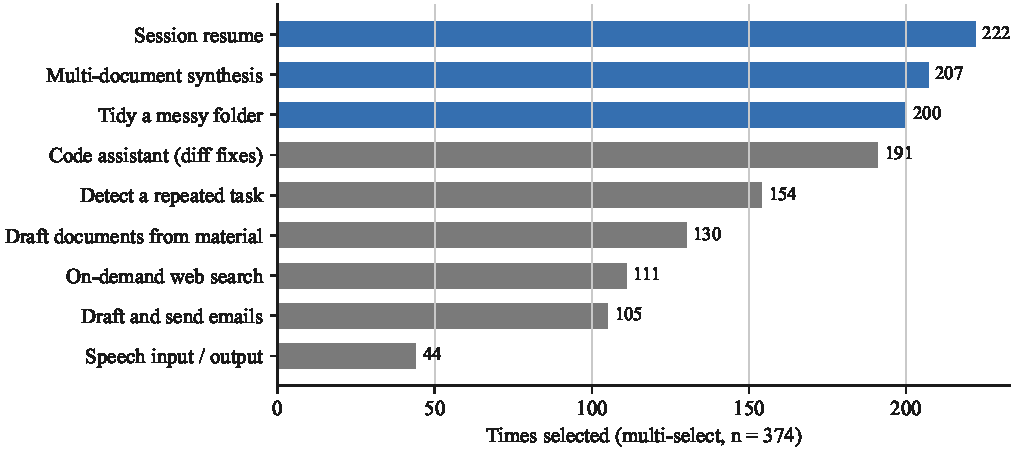
\includegraphics[width=\textwidth]{Figures/fig_features.pdf}
    \caption{Feature demand (n = 374).}
    \label{fig:features}
\end{figure}

Demand is concentrated on session resume, notes synthesis and folder tidy.

\section{Functional Requirements}
The functional requirements describe the external behaviour of the system. Each is stated with the user who exercises it.

\subsection{Workspace Management}
\begin{itemize}
    \item \textbf{FR-1} The system will enable the user to make a folder a workspace, which will record its name, canonical root path, permission level and cloud policy. User: all primary users.
    \item \textbf{FR-2} The system will not resolve any path the canonical form of which is not in the root of an active grant. User: all primary users, indirectly.
    \item \textbf{FR-3} The system will canonicalise a path, including symbolic links and relative segments, and then test whether it is contained in a grant. User: all primary users, indirectly.
    \item \textbf{FR-4} The system will not resolve paths that match a denylist of credential and system locations, even when the path is in a granted folder. User: all primary users, indirectly.
    \item \textbf{FR-5} The system will enable the user to cancel a workspace, which will remove the index entries, embeddings, sessions, memory and rules, but not the files of the user. User: all primary users.
    \item \textbf{FR-6} The system will have an index of the files in each granted workspace, which will be updated incrementally as files change. User: all primary users, indirectly.
\end{itemize}

\subsection{Action Gating and Recovery}
\begin{itemize}
    \item \textbf{FR-7} The system will categorize all the proposed actions into precisely one of four risk levels, which are read, reversible, outward and destructive. User: all primary users, indirectly.
    \item \textbf{FR-8} The system will perform read operations in a granted workspace without authorization. User: all primary users.
    \item \textbf{FR-9} The system will store all reversible actions pending approval, unless the user has already decided to allow that operation in that workspace without prompting. User: all primary users.
    \item \textbf{FR-10} The system will retain all outward actions pending approval in any situation, and will not allow this to be set off. User: all primary users.
    \item \textbf{FR-11} The system will reject all destructive actions, and it will not give any approval route through which it can be done. User: all primary users.
    \item \textbf{FR-12} The system will display, prior to any gated action, a preview of the workspace being impacted, the operations being proposed, the risk level, whether anything is leaving the machine, and whether anything is being deleted. User: all primary users.
    \item \textbf{FR-13} The system will enable the user to approve, approve and remember, edit or reject a pending plan. User: all primary users.
    \item \textbf{FR-14} The system will scope a remembered approval to a single operation in a single workspace, and will never remember an outward or destructive operation. User: all primary users.
    \item \textbf{FR-15} The system will document the reversal of each change prior to the change. User: all primary users, indirectly.
    \item \textbf{FR-16} The system will enable the user to undo an approved plan as a unit, and the steps will be restored in the reverse order. User: all primary users.
    \item \textbf{FR-17} The system will not automatically accept a pending action, by default or under load, by default or by load. User: all primary users, indirectly.
    \item \textbf{FR-18} The system will maintain a record of all proposals, refusals, approvals, rejections and executions in an append-only, hash-chained audit log. User: all primary users; auditor.
\end{itemize}

\subsection{Capability Features}
\begin{itemize}
    \item \textbf{FR-19} The system will provide, on demand, the files that have been recently used in a workspace and the last action that the user took, to allow the work to be restarted. User: all primary users.
    \item \textbf{FR-20} The system will suggest a sorting of files in a folder, and all the moves will be previewed before any is executed. User: all primary users.
    \item \textbf{FR-21} The system will identify a manual sequence that is repeated three or more times and will suggest to automate it, and will not install an automation without the user consent. User: all primary users.
    \item \textbf{FR-22} The system will synthesise content across documents in a workspace, and each claim will be attached with a citation of its source file and location. User: all primary users.
    \item \textbf{FR-23} The system will make unsupported any claim in a synthesis which cannot be traced to a source. User: all primary users.
    \item \textbf{FR-24} The system will respond to questions regarding source code in a workspace and will display any proposed change as a difference, and will never write or execute code independently. User: developer.
    \item \textbf{FR-25} The system will not search the web automatically, but only when an explicit user request is made, and will not search in the background. User: all primary users.
    \item \textbf{FR-26} The system will prepare electronic mail in the form of a draft and will not be sent until the user has approved the draft. User: all primary users.
    \item \textbf{FR-27} The system will create a written document as a new file and will never overwrite an existing one. User: all primary users.
    \item \textbf{FR-28} The system will be able to receive spoken input and give spoken output, with the same approval gates as typed interaction. User: all primary users.
    \item \textbf{FR-29} The system will only record audio when a voice session has been armed by the user. User: all primary users.
\end{itemize}

\subsection{Disclosure and Model Access}
\begin{itemize}
    \item \textbf{FR-30} The system will provide a panel that reports all workspaces granted, files indexed, chunks embedded, facts remembered, sessions retained, automation rule, policy exception, action taken and item of data sent outside the machine. User: all primary users.
    \item \textbf{FR-31} The system will enable the user to remove any item displayed in that panel except the audit log. User: all primary users.
    \item \textbf{FR-32} The default configuration of the system will direct model requests to a local model. User: all primary users, indirectly.
    \item \textbf{FR-33} The system will not send workspace content to a model tier that has been disabled by the cloud policy of the workspace. User: all primary users, indirectly.
    \item \textbf{FR-34} The system will not retrieve any material not within the active grant, and will document each such exclusion. User: all primary users, indirectly.
    \item \textbf{FR-35} The system will generate an inspectable plan without executing it, and will only allow execution by the dispatcher and only where a corresponding policy verdict exists. User: all primary users, indirectly.
\end{itemize}

\section{Quality Attributes}
The quality attributes below declare the properties that the system should possess, along with the method of measuring each of them.

\begin{itemize}
    \item \textbf{QA-1 Confinement.} Any operation that solves a path not within an active grant is an error. Evaluated by tests that seek traversal with relative segments, symbolic links to external the grant, absolute paths, and sibling directories with a common prefix in their name, all of which should be denied and recorded.
    \item \textbf{QA-2 Non-destructiveness.} There is no execution path that removes or overwrites user data without a snapshot. Evaluated by examining the operations registered by the dispatcher and by tests that destructive operations are denied instead of gated.
    \item \textbf{QA-3 Recoverability.} Any approved reversible plan is reversible. Evaluated by tests that run a plan, run it in reverse, and compare the state of the filesystem after running the plan to the state before running the plan.
    \item \textbf{QA-4 Transparency.} All the system contains is reportable and, except the audit log, deletable. Evaluated by comparing the counts reported by the panel with direct queries of each store..
    \item \textbf{QA-5 Auditability.} The history of activities cannot be changed without being noticed. Evaluated by re-computing the hash chain and ensuring that any alteration or deletion of an entry destroys it.
    \item \textbf{QA-6 Responsiveness.} The interactive path does not block on background work. Assessed by measuring time to first token while an initial workspace ingestion is in progress.
    \item \textbf{QA-7 Degradability.} The loss of any external capability results in a declared constraint and not a failure. Compared to the degradation contract in Chapter 6.
    \item \textbf{QA-8 Modality parity.} Voice interaction uses the same gates as typed interaction. Evaluated by ensuring that the voice mode introduction did not need any extra approval gate.
\end{itemize}

\section{Non-Functional Requirements}
\begin{itemize}
    \item \textbf{NFR-1 Performance.} The interactive path will generate a first token in less than one second with a local model and in less than two seconds with a cloud model, on the reference hardware defined in Section 4.7.
    \item \textbf{NFR-2 Performance.} Incremental index updates will be debounced and will not block interactive requests. Modifying a single line of a file will result in the re-embedding of only the modified chunk.
    \item \textbf{NFR-3 Capacity.} The system will run under adjustable limits on memory, index size and processor share, and will be usable on a consumer laptop during indexing.
    \item \textbf{NFR-4 Concurrency.} The system has a single interactive user per host instance. Background work will be implemented using a bounded priority queue that will drop the lowest-priority work when full instead of expanding indefinitely.
    \item \textbf{NFR-5 Availability.} The basic functionality will be maintained without the internet. Actions that need the network will fail as explicit, retriable actions instead of being silently dropped.
    \item \textbf{NFR-6 Privacy.} User documents, embeddings, session history, memory, credentials and audit logs will not be sent to any server operated by the project.
    \item \textbf{NFR-7 Security.} The credentials will be stored in the operating system keyring and will never be written to the system own storage tree. At rest, data will be encrypted.
    \item \textbf{NFR-8 Security.} The system will not open an inbound listening port except on the loopback interface.
    \item \textbf{NFR-9 Usability.} The granularity of approval will be user-configurable, allowing approval of all actions, approval by category, or session-based trust following initial approvals.
    \item \textbf{NFR-10 Usability.} Background work will report visible, cancellable progress instead of an indeterminate indicator.
    \item \textbf{NFR-11 Reusability.} Capability features will be provided as a uniform tool contract, with a new feature being added without changing the gateway.
    \item \textbf{NFR-12 Extensibility.} Model providers will be configuration, not code branches, such that any compatible endpoint can be registered without changing the router.
    \item \textbf{NFR-13 Portability.} The system will be based on Windows, macOS and Linux, and will not rely on any platform-specific filesystem behaviour to provide its confinement guarantee.
    \item \textbf{NFR-14 Maintainability.} Path resolution will be in one component and execution in one other, such that every guarantee has a single enforcement point.
\end{itemize}

\section{Assumptions}
The specification rests on the following assumptions.

\begin{itemize}
    \item The user is an individual who has his/her own machine and has the right to access the folders of his/her choice.
    \item The host machine has enough resources to execute a small local language model, or the user has configured cloud fallback on the workspaces in question.
    \item The operating system offers a keyring that is appropriate to store credentials and a canonicalisation algorithm that correctly resolves symbolic links.
    \item The metadata that incremental indexing relies on, i.e. modification times and stable path identity, are supported by the filesystem.
    \item Workspaces that are granted as folders are not concurrently modified by some other automated process in a way that would invalidate a snapshot between its capture and the next operation.
    \item The user can read a preview of what will happen and make a decision about it, which the literature indicates is an assumption and not a guarantee and which the assessment should investigate.
    \item The documents in a workspace can be adversarial, as a file can be created by any source, and the design thus considers retrieved content as data, not as instruction.
\end{itemize}

\section{Use Cases}
This section presents the use cases that exercise the central functionality of the system or that illustrate a delicate point of the architecture. Four are given: granting a workspace, which establishes the boundary; tidying a folder, which exercises the gating and recovery path end to end; attempting to reach outside a workspace, which demonstrates the confinement guarantee; and sending mail, which demonstrates that an outward action cannot be configured past its gate.

{\Needspace*{3\baselineskip}
\begin{longtable}{|lllll|}
\caption{Use case UC-1: grant a folder as a workspace.}\label{tab:uc1}\\*
\endfirsthead
\caption[]{continued from previous page}\\*
\endhead
\hline
\multicolumn{2}{|l|}{\textbf{Name}} &
  \multicolumn{3}{l|}{UC-1 Grant a folder as a workspace} \\ \hline
\multicolumn{2}{|l|}{\textbf{Actors}} &
  \multicolumn{3}{l|}{Student, Developer, Freelancer} \\ \hline
\multicolumn{2}{|l|}{\textbf{Summary}} &
  \multicolumn{3}{l|}{\begin{tabular}[c]{@{}l@{}}The user selects a folder and opts it in as a workspace. The system records\\ the grant, indexes the folder, and reports what it now holds.\end{tabular}} \\ \hline
\multicolumn{2}{|l|}{\textbf{Pre-Conditions}} &
  \multicolumn{3}{l|}{\begin{tabular}[c]{@{}l@{}}The folder exists and is readable by the user.\\ The folder is not already granted.\end{tabular}} \\ \hline
\multicolumn{2}{|l|}{\textbf{Post-Conditions}} &
  \multicolumn{3}{l|}{\begin{tabular}[c]{@{}l@{}}A grant exists with a canonical root, a permission level and a cloud policy.\\ The folder's files are indexed and the grant is recorded in the audit log.\end{tabular}} \\ \hline
\multicolumn{2}{|l|}{\textbf{\begin{tabular}[c]{@{}l@{}}Special\\ Requirements\end{tabular}}} &
  \multicolumn{3}{l|}{\begin{tabular}[c]{@{}l@{}}The root is stored canonically, so that a later symbolic link cannot alter\\ the region the grant covers.\end{tabular}} \\ \hline
\multicolumn{5}{|c|}{\textbf{Basic Flow}} \\ \hline
\multicolumn{3}{|c|}{\textbf{Actor Action}} &
  \multicolumn{2}{c|}{\textbf{System Response}} \\ \hline
\multicolumn{1}{|l|}{1} &
  \multicolumn{2}{l|}{\begin{tabular}[c]{@{}l@{}}The user selects a folder\\ and names it.\end{tabular}} &
  \multicolumn{1}{l|}{2} &
  \begin{tabular}[c]{@{}l@{}}The system canonicalises the path and records\\ the grant with its permission and cloud policy.\end{tabular} \\ \hline
\multicolumn{1}{|l|}{3} &
  \multicolumn{2}{l|}{\begin{tabular}[c]{@{}l@{}}The user confirms the\\ permission level.\end{tabular}} &
  \multicolumn{1}{l|}{4} &
  \begin{tabular}[c]{@{}l@{}}The system indexes the folder in the background,\\ reporting visible progress, and writes the grant\\ to the audit log.\end{tabular} \\ \hline
\multicolumn{5}{|c|}{\textbf{Alternative Flow}} \\ \hline
\multicolumn{1}{|l|}{1-A} &
  \multicolumn{2}{l|}{\begin{tabular}[c]{@{}l@{}}The user selects a folder\\ already granted.\end{tabular}} &
  \multicolumn{1}{l|}{2-A} &
  \begin{tabular}[c]{@{}l@{}}The system reports that the folder is already a\\ workspace and makes no change.\end{tabular} \\ \hline
\end{longtable}
}

{\Needspace*{3\baselineskip}
\begin{longtable}{|lllll|}
\caption{Use case UC-2: tidy a folder.}\label{tab:uc2}\\*
\endfirsthead
\caption[]{continued from previous page}\\*
\endhead
\hline
\multicolumn{2}{|l|}{\textbf{Name}} &
  \multicolumn{3}{l|}{UC-2 Tidy a folder} \\ \hline
\multicolumn{2}{|l|}{\textbf{Actors}} &
  \multicolumn{3}{l|}{Student, Developer, Freelancer} \\ \hline
\multicolumn{2}{|l|}{\textbf{Summary}} &
  \multicolumn{3}{l|}{\begin{tabular}[c]{@{}l@{}}The user asks the system to tidy a folder. The system proposes a plan of\\ moves, the user previews and approves it, and the system executes it with\\ undo available afterwards.\end{tabular}} \\ \hline
\multicolumn{2}{|l|}{\textbf{Pre-Conditions}} &
  \multicolumn{3}{l|}{\begin{tabular}[c]{@{}l@{}}The folder lies within a granted workspace with write permission.\\ The workspace has been indexed.\end{tabular}} \\ \hline
\multicolumn{2}{|l|}{\textbf{Post-Conditions}} &
  \multicolumn{3}{l|}{\begin{tabular}[c]{@{}l@{}}The approved moves have been performed, the inverse of each is recorded,\\ and the plan may be reversed as one unit. Nothing has been deleted.\end{tabular}} \\ \hline
\multicolumn{2}{|l|}{\textbf{\begin{tabular}[c]{@{}l@{}}Special\\ Requirements\end{tabular}}} &
  \multicolumn{3}{l|}{\begin{tabular}[c]{@{}l@{}}The snapshot is recorded before any move is performed. Undo operates at\\ the granularity of the plan, not of the individual move.\end{tabular}} \\ \hline
\multicolumn{5}{|c|}{\textbf{Basic Flow}} \\ \hline
\multicolumn{3}{|c|}{\textbf{Actor Action}} &
  \multicolumn{2}{c|}{\textbf{System Response}} \\ \hline
\multicolumn{1}{|l|}{1} &
  \multicolumn{2}{l|}{\begin{tabular}[c]{@{}l@{}}The user asks the system\\ to tidy a folder.\end{tabular}} &
  \multicolumn{1}{l|}{2} &
  \begin{tabular}[c]{@{}l@{}}The system lists the folder, reads metadata, and\\ produces a plan of proposed moves.\end{tabular} \\ \hline
\multicolumn{1}{|l|}{} &
  \multicolumn{2}{l|}{} &
  \multicolumn{1}{l|}{3} &
  \begin{tabular}[c]{@{}l@{}}The system classifies each step, and presents a\\ preview stating the risk tier, that nothing leaves\\ the machine and that nothing is deleted.\end{tabular} \\ \hline
\multicolumn{1}{|l|}{4} &
  \multicolumn{2}{l|}{\begin{tabular}[c]{@{}l@{}}The user reviews the moves\\ and approves the plan.\end{tabular}} &
  \multicolumn{1}{l|}{5} &
  \begin{tabular}[c]{@{}l@{}}The system records the inverse of each move,\\ performs the moves, writes the audit entries and\\ reports that undo is available.\end{tabular} \\ \hline
\multicolumn{5}{|c|}{\textbf{Alternative Flow}} \\ \hline
\multicolumn{1}{|l|}{4-A} &
  \multicolumn{2}{l|}{The user rejects the plan.} &
  \multicolumn{1}{l|}{5-A} &
  \begin{tabular}[c]{@{}l@{}}The system performs nothing, records the\\ rejection in the audit log and halts cleanly.\end{tabular} \\ \hline
\multicolumn{1}{|l|}{4-B} &
  \multicolumn{2}{l|}{\begin{tabular}[c]{@{}l@{}}The user approves, then\\ later requests undo.\end{tabular}} &
  \multicolumn{1}{l|}{5-B} &
  \begin{tabular}[c]{@{}l@{}}The system reverses every move in the plan in\\ reverse order and reports any step it could not\\ reverse.\end{tabular} \\ \hline
\end{longtable}
}

{\Needspace*{3\baselineskip}
\begin{longtable}{|lllll|}
\caption{Use case UC-3: attempt to reach outside a workspace.}\label{tab:uc3}\\*
\endfirsthead
\caption[]{continued from previous page}\\*
\endhead
\hline
\multicolumn{2}{|l|}{\textbf{Name}} &
  \multicolumn{3}{l|}{UC-3 Attempt to reach outside a workspace} \\ \hline
\multicolumn{2}{|l|}{\textbf{Actors}} &
  \multicolumn{3}{l|}{Capability service; indirectly, an adversarial document} \\ \hline
\multicolumn{2}{|l|}{\textbf{Summary}} &
  \multicolumn{3}{l|}{\begin{tabular}[c]{@{}l@{}}A proposed action references a path outside the grant, whether through a\\ relative segment, a symbolic link or an absolute path. The system refuses it\\ and records the attempt.\end{tabular}} \\ \hline
\multicolumn{2}{|l|}{\textbf{Pre-Conditions}} &
  \multicolumn{3}{l|}{A workspace is granted and active.} \\ \hline
\multicolumn{2}{|l|}{\textbf{Post-Conditions}} &
  \multicolumn{3}{l|}{\begin{tabular}[c]{@{}l@{}}No filesystem access occurred outside the grant. The refusal is recorded in\\ the audit log with its reason.\end{tabular}} \\ \hline
\multicolumn{2}{|l|}{\textbf{\begin{tabular}[c]{@{}l@{}}Special\\ Requirements\end{tabular}}} &
  \multicolumn{3}{l|}{\begin{tabular}[c]{@{}l@{}}Canonicalisation precedes the containment test, so that a path which merely\\ appears contained is resolved to its true location first.\end{tabular}} \\ \hline
\multicolumn{5}{|c|}{\textbf{Basic Flow}} \\ \hline
\multicolumn{3}{|c|}{\textbf{Actor Action}} &
  \multicolumn{2}{c|}{\textbf{System Response}} \\ \hline
\multicolumn{1}{|l|}{1} &
  \multicolumn{2}{l|}{\begin{tabular}[c]{@{}l@{}}A service requests a path\\ containing a traversal\\ segment.\end{tabular}} &
  \multicolumn{1}{l|}{2} &
  \begin{tabular}[c]{@{}l@{}}The broker canonicalises the path and finds it\\ outside the grant root.\end{tabular} \\ \hline
\multicolumn{1}{|l|}{} &
  \multicolumn{2}{l|}{} &
  \multicolumn{1}{l|}{3} &
  \begin{tabular}[c]{@{}l@{}}The broker records the refusal and raises it, so no\\ access occurs.\end{tabular} \\ \hline
\multicolumn{5}{|c|}{\textbf{Alternative Flow}} \\ \hline
\multicolumn{1}{|l|}{1-A} &
  \multicolumn{2}{l|}{\begin{tabular}[c]{@{}l@{}}The path is a symbolic\\ link whose target lies\\ outside the grant.\end{tabular}} &
  \multicolumn{1}{l|}{2-A} &
  \begin{tabular}[c]{@{}l@{}}Canonicalisation resolves the link before the\\ containment test, so the refusal is identical.\end{tabular} \\ \hline
\multicolumn{1}{|l|}{1-B} &
  \multicolumn{2}{l|}{\begin{tabular}[c]{@{}l@{}}The path names a\\ credential file inside\\ the grant.\end{tabular}} &
  \multicolumn{1}{l|}{2-B} &
  \begin{tabular}[c]{@{}l@{}}The deny list refuses it even though it lies within\\ the granted folder.\end{tabular} \\ \hline
\end{longtable}
}

{\Needspace*{3\baselineskip}
\begin{longtable}{|lllll|}
\caption{Use case UC-4: draft and send electronic mail.}\label{tab:uc4}\\*
\endfirsthead
\caption[]{continued from previous page}\\*
\endhead
\hline
\multicolumn{2}{|l|}{\textbf{Name}} &
  \multicolumn{3}{l|}{UC-4 Draft and send electronic mail} \\ \hline
\multicolumn{2}{|l|}{\textbf{Actors}} &
  \multicolumn{3}{l|}{Freelancer, Student, Developer} \\ \hline
\multicolumn{2}{|l|}{\textbf{Summary}} &
  \multicolumn{3}{l|}{\begin{tabular}[c]{@{}l@{}}The user asks the system to prepare a message. The system drafts it and\\ holds it until the user approves the exact content and recipient.\end{tabular}} \\ \hline
\multicolumn{2}{|l|}{\textbf{Pre-Conditions}} &
  \multicolumn{3}{l|}{\begin{tabular}[c]{@{}l@{}}A mail account is configured and its credentials are held in the keyring.\\ Any material referenced lies within a granted workspace.\end{tabular}} \\ \hline
\multicolumn{2}{|l|}{\textbf{Post-Conditions}} &
  \multicolumn{3}{l|}{\begin{tabular}[c]{@{}l@{}}The message is sent only if approved. The egress is recorded in the audit\\ log with its recipient and time.\end{tabular}} \\ \hline
\multicolumn{2}{|l|}{\textbf{\begin{tabular}[c]{@{}l@{}}Special\\ Requirements\end{tabular}}} &
  \multicolumn{3}{l|}{\begin{tabular}[c]{@{}l@{}}This gate is not configurable. A remembered approval cannot be recorded\\ for an outward operation.\end{tabular}} \\ \hline
\multicolumn{5}{|c|}{\textbf{Basic Flow}} \\ \hline
\multicolumn{3}{|c|}{\textbf{Actor Action}} &
  \multicolumn{2}{c|}{\textbf{System Response}} \\ \hline
\multicolumn{1}{|l|}{1} &
  \multicolumn{2}{l|}{\begin{tabular}[c]{@{}l@{}}The user asks for a\\ message to be prepared.\end{tabular}} &
  \multicolumn{1}{l|}{2} &
  \begin{tabular}[c]{@{}l@{}}The system drafts the message and classifies the\\ send step as an outward action.\end{tabular} \\ \hline
\multicolumn{1}{|l|}{} &
  \multicolumn{2}{l|}{} &
  \multicolumn{1}{l|}{3} &
  \begin{tabular}[c]{@{}l@{}}The system presents the recipient, subject and full\\ body for approval.\end{tabular} \\ \hline
\multicolumn{1}{|l|}{4} &
  \multicolumn{2}{l|}{\begin{tabular}[c]{@{}l@{}}The user reads the draft\\ and approves it.\end{tabular}} &
  \multicolumn{1}{l|}{5} &
  \begin{tabular}[c]{@{}l@{}}The system sends the message and records the\\ egress in the audit log.\end{tabular} \\ \hline
\multicolumn{5}{|c|}{\textbf{Alternative Flow}} \\ \hline
\multicolumn{1}{|l|}{4-A} &
  \multicolumn{2}{l|}{\begin{tabular}[c]{@{}l@{}}The user requests that the\\ approval be remembered.\end{tabular}} &
  \multicolumn{1}{l|}{5-A} &
  \begin{tabular}[c]{@{}l@{}}The system declines to record the rule, because\\ outward operations are never remembered.\end{tabular} \\ \hline
\multicolumn{1}{|l|}{4-B} &
  \multicolumn{2}{l|}{The user rejects the draft.} &
  \multicolumn{1}{l|}{5-B} &
  \begin{tabular}[c]{@{}l@{}}Nothing is sent and the rejection is recorded.\end{tabular} \\ \hline
\end{longtable}
}

Nothing is sent and the rejection is recorded. draft. The four use cases together exercise the principal architectural elements. UC-1 establishes the boundary and the index. UC-2 traverses classification, preview, approval, snapshot, execution, audit and reversal, which is the full length of the request lifecycle. UC-3 demonstrates the confinement guarantee against the three forms of escape a bounded system must resist. UC-4 demonstrates that the outward gate is a property of the architecture rather than a configurable preference.

\section{Hardware and Software Requirements}
\subsection{Hardware Requirements}
Table~\ref{tab:hardware} states the minimum and recommended hardware for the host machine. The minimum configuration is intended to run the system with a small local model, and the recommended configuration is the reference against which the performance requirements in Section 4.4 are measured.

{\Needspace*{7\baselineskip}
\begin{longtable}{|p{3.4cm}|p{4.8cm}|p{5.4cm}|}
\caption{Host hardware requirements.}\label{tab:hardware}\\*
\hline
\textbf{Component} & \textbf{Minimum} & \textbf{Recommended} \\*
\hline
\endfirsthead
\caption[]{continued from previous page}\\*
\hline
\textbf{Component} & \textbf{Minimum} & \textbf{Recommended} \\*
\hline
\endhead
\hline
Processor & Quad-core, 2.0 GHz & Eight-core, 2.5 GHz or higher \\
\hline
Memory & 8 GB & 16 GB or more, permitting a larger local model to remain resident \\
\hline
Storage & 10 GB free, solid-state & 25 GB free, solid-state, for indexes and snapshots \\
\hline
Graphics & Not required; inference on processor & Dedicated graphics with 6 GB memory or more, for local inference \\
\hline
Audio & Microphone and output device, for the voice mode & As minimum \\
\hline
Network & Not required for core operation & Broadband, for cloud fallback and web search \\
\hline
\end{longtable}
}

\subsection{Software Requirements}
Table~\ref{tab:software} states the software required to develop and operate the system, together with the purpose each serves.

{\Needspace*{7\baselineskip}
\begin{longtable}{|p{3.6cm}|p{3.0cm}|p{6.2cm}|}
\caption{Software requirements.}\label{tab:software}\\*
\hline
\textbf{Component} & \textbf{Version} & \textbf{Purpose} \\*
\hline
\endfirsthead
\caption[]{continued from previous page}\\*
\hline
\textbf{Component} & \textbf{Version} & \textbf{Purpose} \\*
\hline
\endhead
\hline
Operating system & Windows 10 or later, macOS 12 or later, or a current Linux distribution & Host platform \\
\hline
Python & 3.11 or later & Implementation language for the entire system \\
\hline
LangGraph \cite{ref:langgraph} & Current & Multi-step planning with an explicit pause before consequential calls \\
\hline
Ollama \cite{ref:ollama} & Current & Local model runtime, the default inference tier \\
\hline
SQLite \cite{ref:sqlite} & 3.35 or later & Local system of record for metadata, sessions, rules and audit \\
\hline
Local vector index & Current & Per-workspace embedding storage and retrieval \\
\hline
Typer & 0.12 or later & Command line interface \\
\hline
Gradio & 6.0 or later & Local graphical control panel served on the loopback interface \\
\hline
Watchdog & 4.0 or later & Filesystem change detection for incremental indexing \\
\hline
Operating system keyring & Platform-provided & Credential storage outside the system's own tree \\
\hline
Pytest & 8.0 or later & Automated verification of the boundary, policy, approval and undo guarantees \\
\hline
\end{longtable}
}

\section{Graphical User Interface}
The system has three surfaces sharing a single view model, such that the same state is seen no matter how it is arrived at. The command line surface is scriptable and the surface on which configuration and diagnosis is done. The main surface is the local graphical control panel, which is only served on the loopback interface. The optional remote progressive web application, as outlined in Chapter 6, displays the same view model on a different device and does not have any extra privilege.

The control panel has five views. The chat view takes a typed or spoken request and shows the response along with any plan generated. The approval view shows a pending plan with its preview, the workspace to be affected, the operations to be performed, the risk level, anything leaves the machine or anything is deleted, and approve, approve and remember, edit and reject. The disclosure view enforces FR-30 and FR-31, enumerating all types of held data and their number and allowing deletion. FR-1 and FR-5 are implemented by the workspace view, which lists grants and provides revocation. The activity view presents the audit log and the undo history, implementing FR-16 and FR-18.

Navigation is a request lifecycle. A user starts in the chat view, is redirected to the approval view when a plan needs a decision, and is redirected to the chat view with the result and an undo affordance. The disclosure, workspace and activity views can be accessed at any time and are not included in the request path. The implementation is annotated with each view and the requirements it fulfills, so that the interface can be checked against the specification instead of being evaluated by impression.

The flow of navigation is presented in Figure~\ref{fig:nav}, and the screens of the main surface are presented in Figures~\ref{fig:gui} to \ref{fig:gui8}. The request path (FR-8 to FR-16 and FR-28) is covered by the Work screen, the Folders screen covers FR-1 and FR-5, and the What it knows screen covers FR-30 and FR-31. The model, mail and remote access options, and the interface can be changed to a dark theme in the Settings screen.

\begin{figure}[H]
\centering
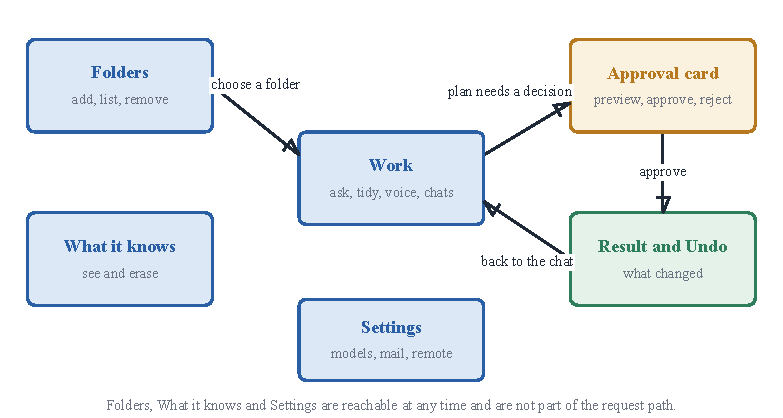
\includegraphics[width=0.95\textwidth]{Figures/fig_nav.pdf}
\caption{Navigation flow of the control panel.}
\label{fig:nav}
\end{figure}

The Work screen is where a request begins. The user chooses a folder, types or speaks what is wanted and presses Ask, or uses one of the shortcut buttons for a tidy-up, for what changed and for repeated tasks. The voice controls sit in a collapsible panel, and the saved chats are listed in the sidebar.

\begin{figure}[H]
\centering
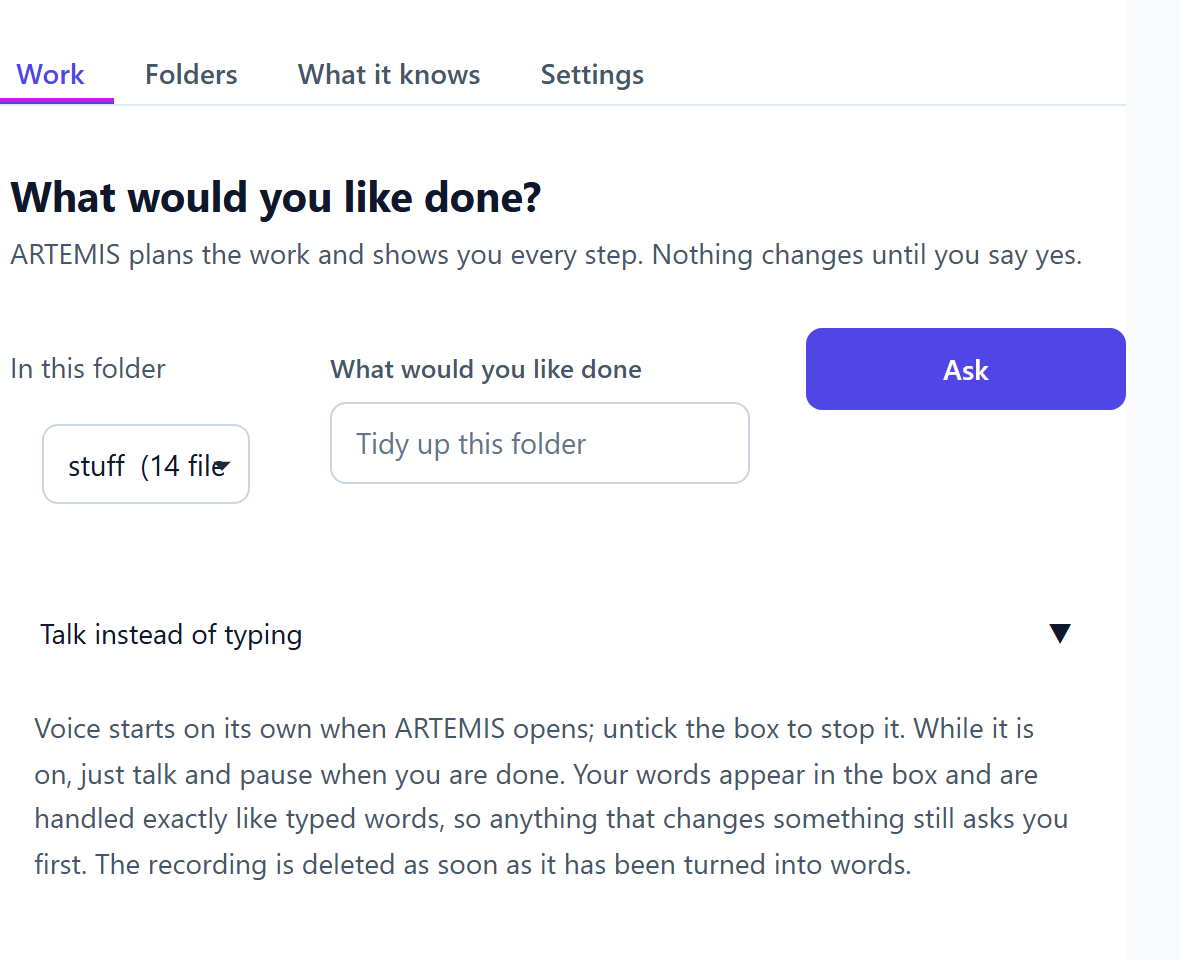
\includegraphics[width=0.64\textwidth]{Figures/s_work.png}
\caption{Work screen: ask, tidy and voice.}
\label{fig:gui}
\end{figure}

The Folders screen lets the user opt a folder in by typing its path or browsing to it. Each granted folder is listed with the number of files it holds, the permission it carries and whether cloud models are allowed for it. A folder that has not been added here cannot be seen by the assistant at all.

\begin{figure}[H]
\centering
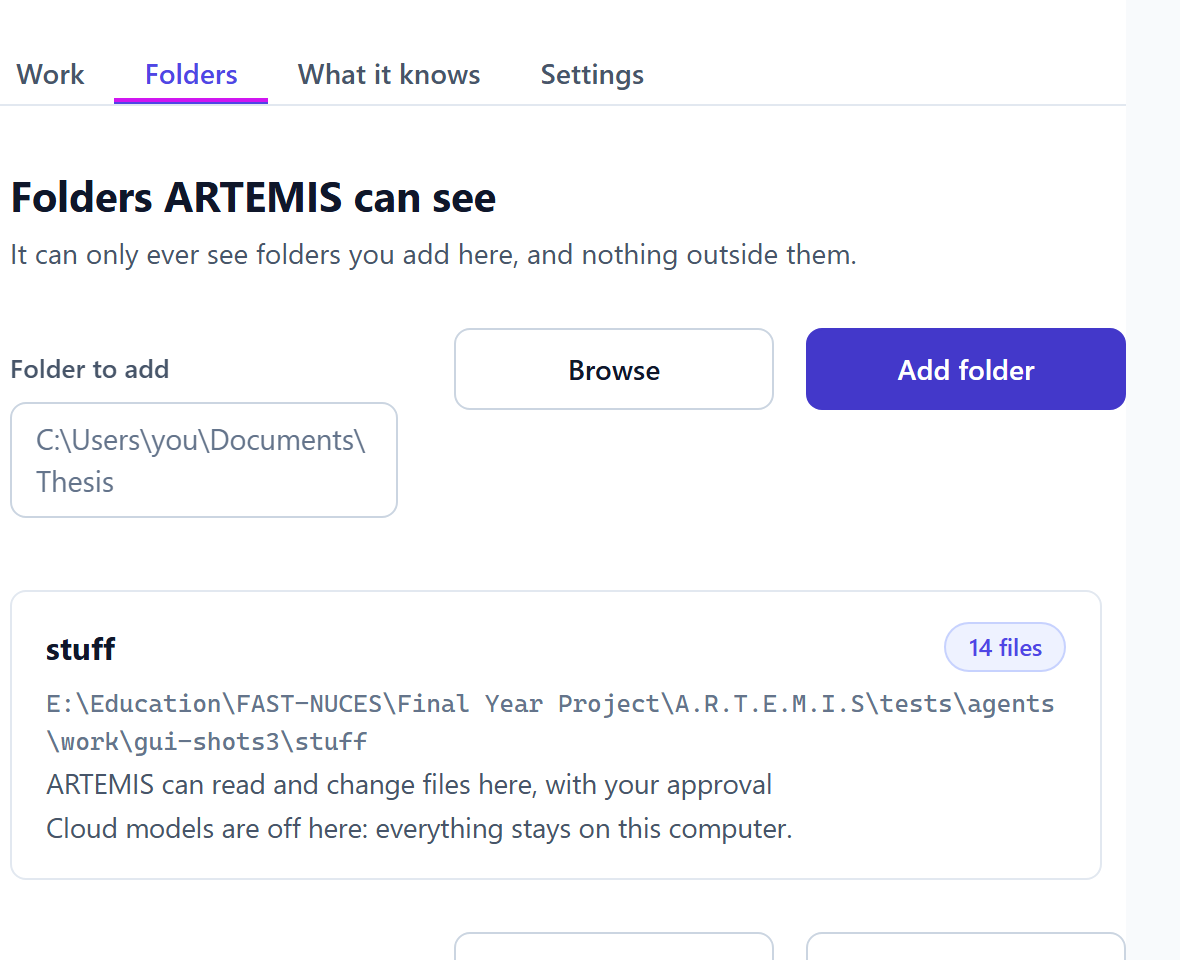
\includegraphics[width=0.64\textwidth]{Figures/s_folders.png}
\caption{Folders screen: add and list folders.}
\label{fig:gui2}
\end{figure}

The What it knows screen implements the disclosure requirement. For the chosen folder it lists every file the assistant has indexed, offers a check for changes, and offers a button that forgets the folder. Forgetting removes what the assistant holds and never touches the user's own files.

\begin{figure}[H]
\centering
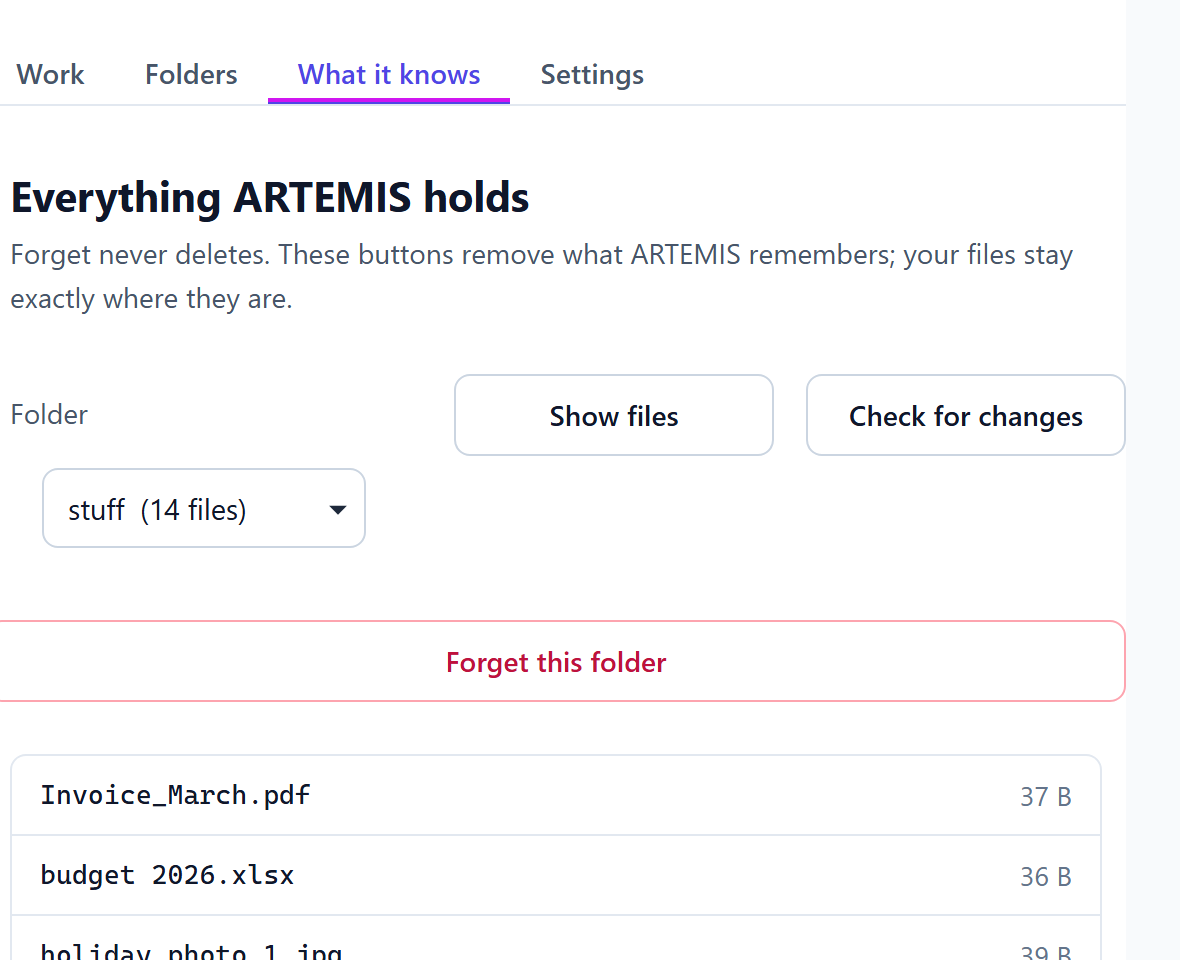
\includegraphics[width=0.64\textwidth]{Figures/s_knows.png}
\caption{What it knows screen: see and erase.}
\label{fig:gui3}
\end{figure}

When a request would change files, the assistant does not act. It shows a plan in plain words and three choices: Approve, Approve and do not ask again for this kind of change, or No, leave it. Nothing has happened until the user presses one of them.

\begin{figure}[H]
\centering
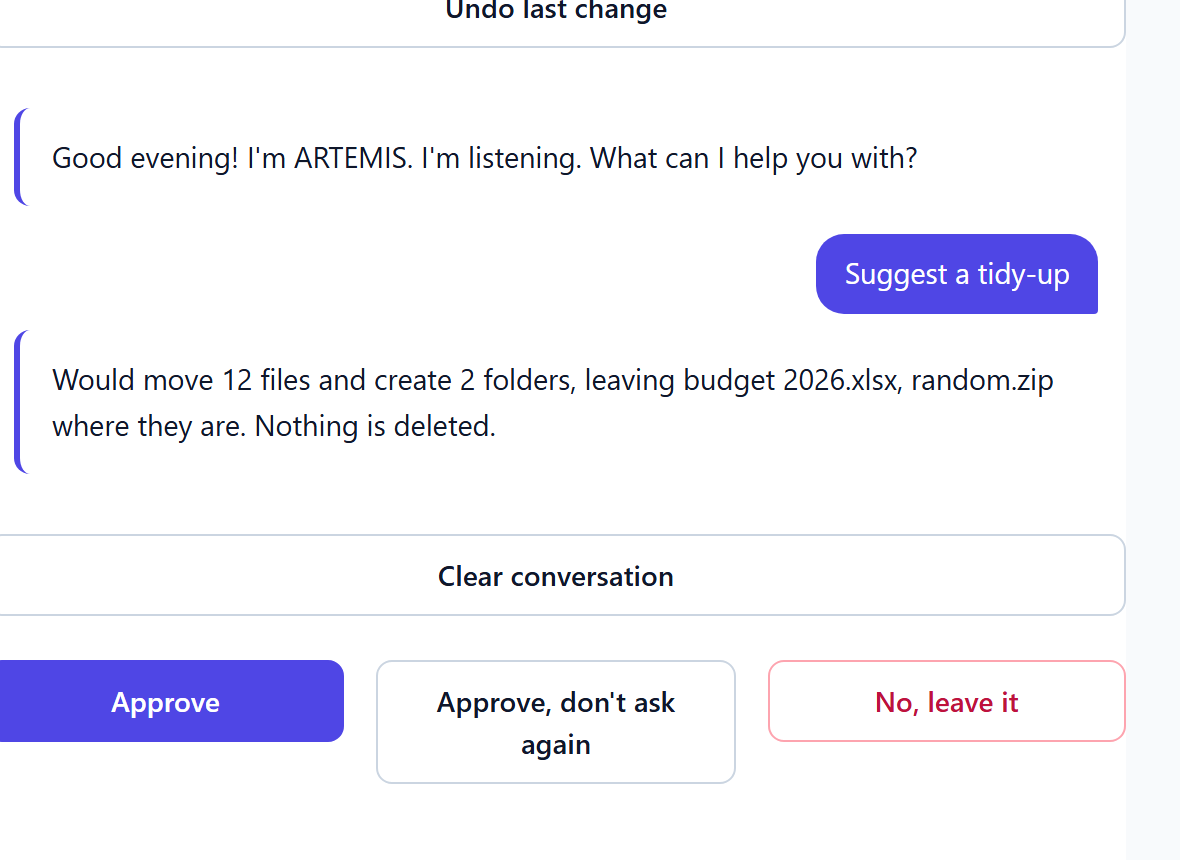
\includegraphics[width=0.64\textwidth]{Figures/s_approval.png}
\caption{Approval card for a tidy-up plan.}
\label{fig:gui4}
\end{figure}

After approval the assistant reports what it did, and the Undo last change button reverses the whole plan as one unit. Here a tidy-up that created two folders and moved twelve files is undone in a single step.

\begin{figure}[H]
\centering
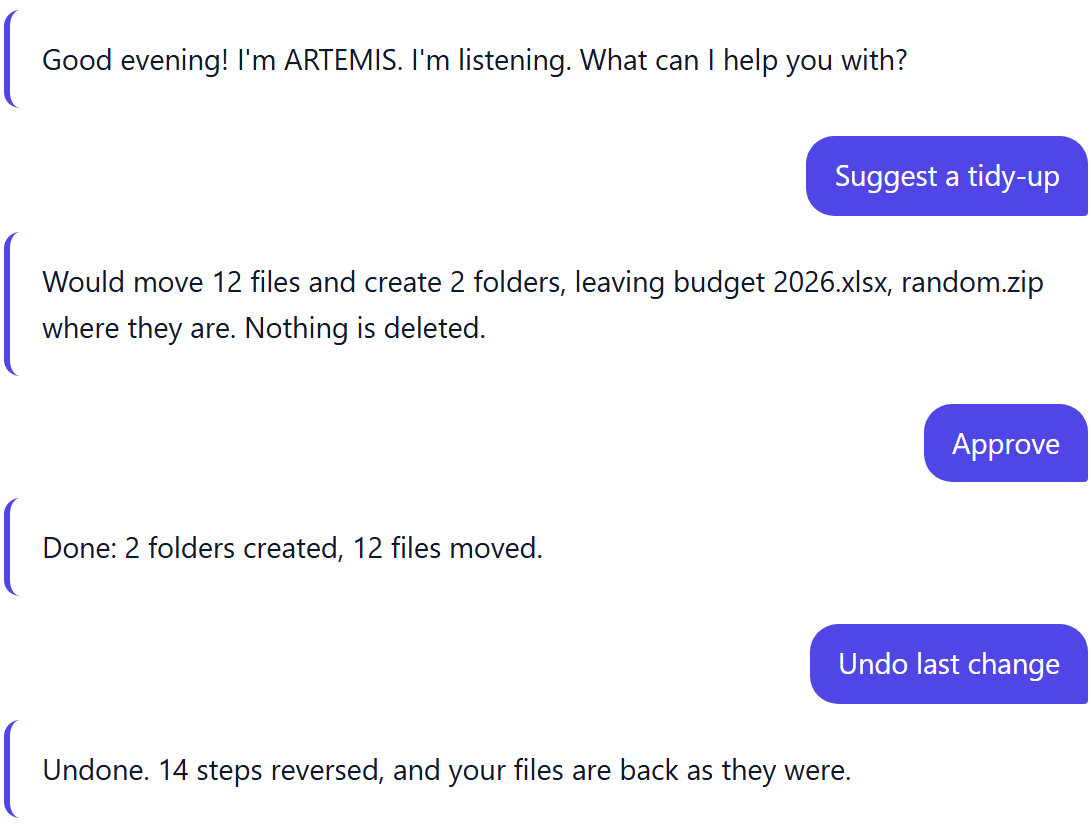
\includegraphics[width=0.64\textwidth]{Figures/s_undo.png}
\caption{A tidy-up, its approval and its undo.}
\label{fig:gui5}
\end{figure}

The Settings screen holds the choices that are not part of everyday use: where the assistant keeps what it knows, which models it may use, the mail account, and the remote access controls.

\begin{figure}[H]
\centering
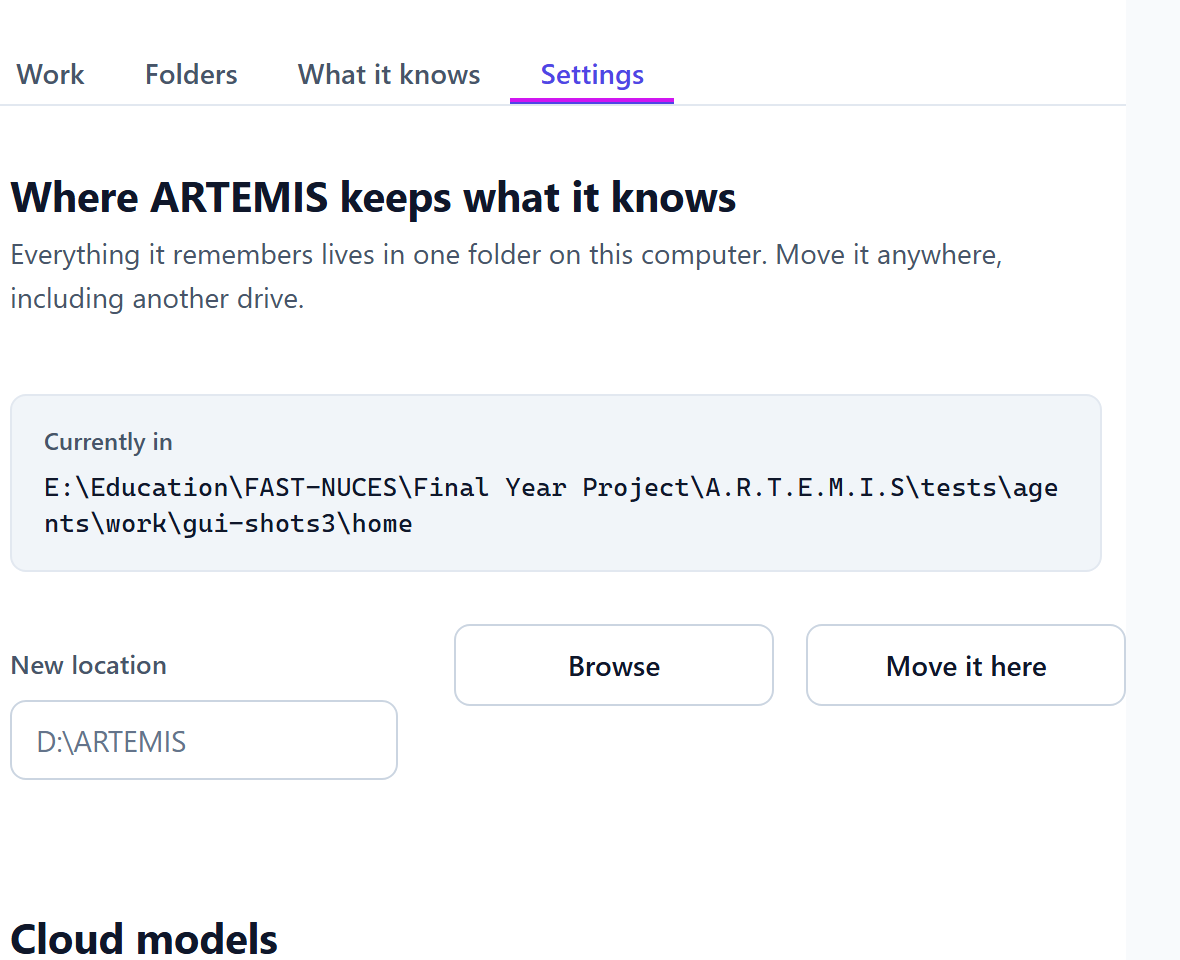
\includegraphics[width=0.64\textwidth]{Figures/s_settings.png}
\caption{Settings screen: data location and cloud models.}
\label{fig:gui6}
\end{figure}

Remote access is optional and off until the user connects to a relay. The screen states that messages are scrambled on the phone and only unscrambled on the computer, and it lists the folders a paired device may use, none by default.

\begin{figure}[H]
\centering
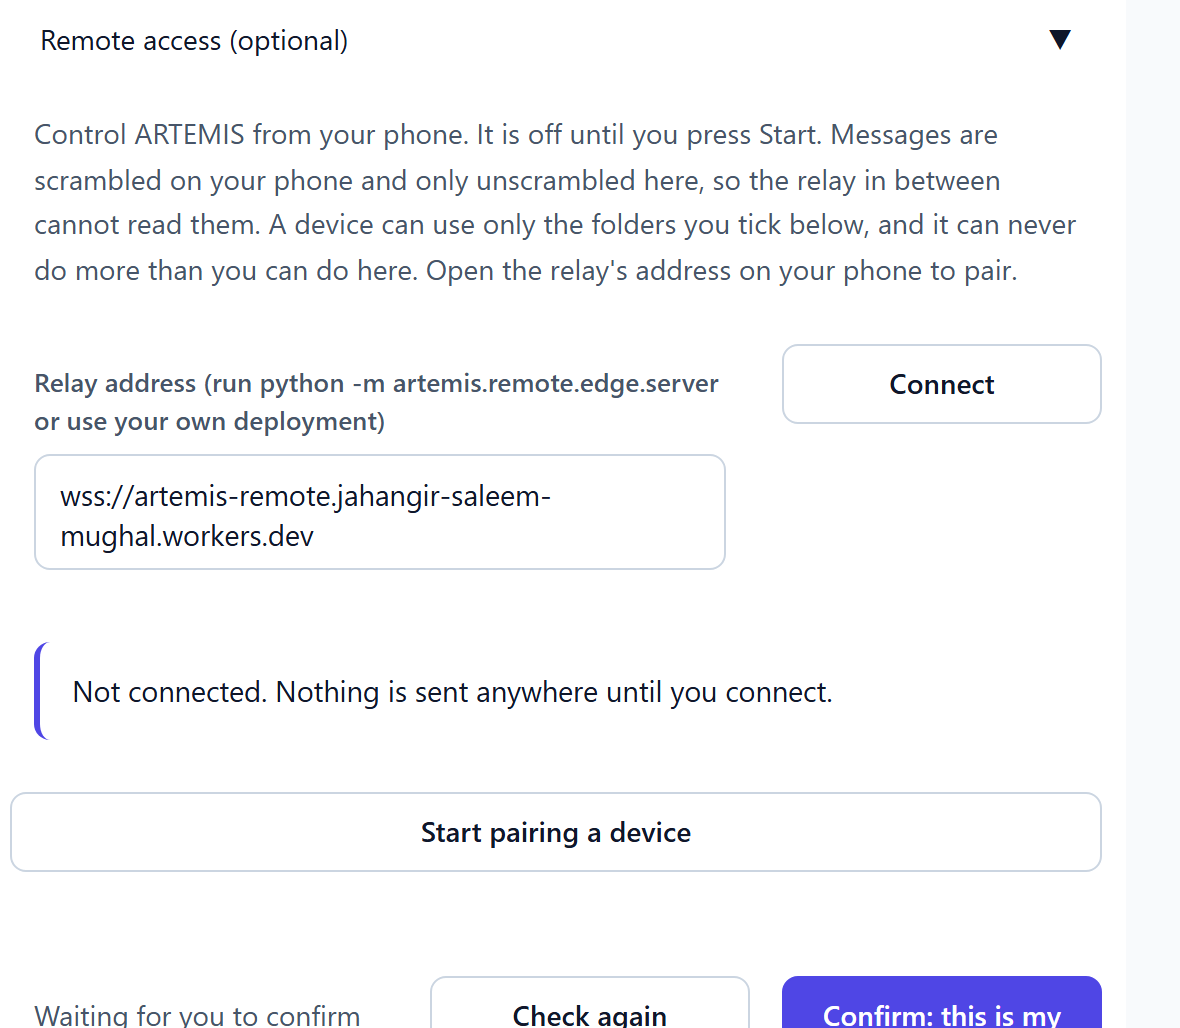
\includegraphics[width=0.64\textwidth]{Figures/s_remote.png}
\caption{Remote access controls in Settings.}
\label{fig:gui7}
\end{figure}

The interface can be switched between a light and a dark theme with one button, and the same screens and controls are shown in both.

\begin{figure}[H]
\centering
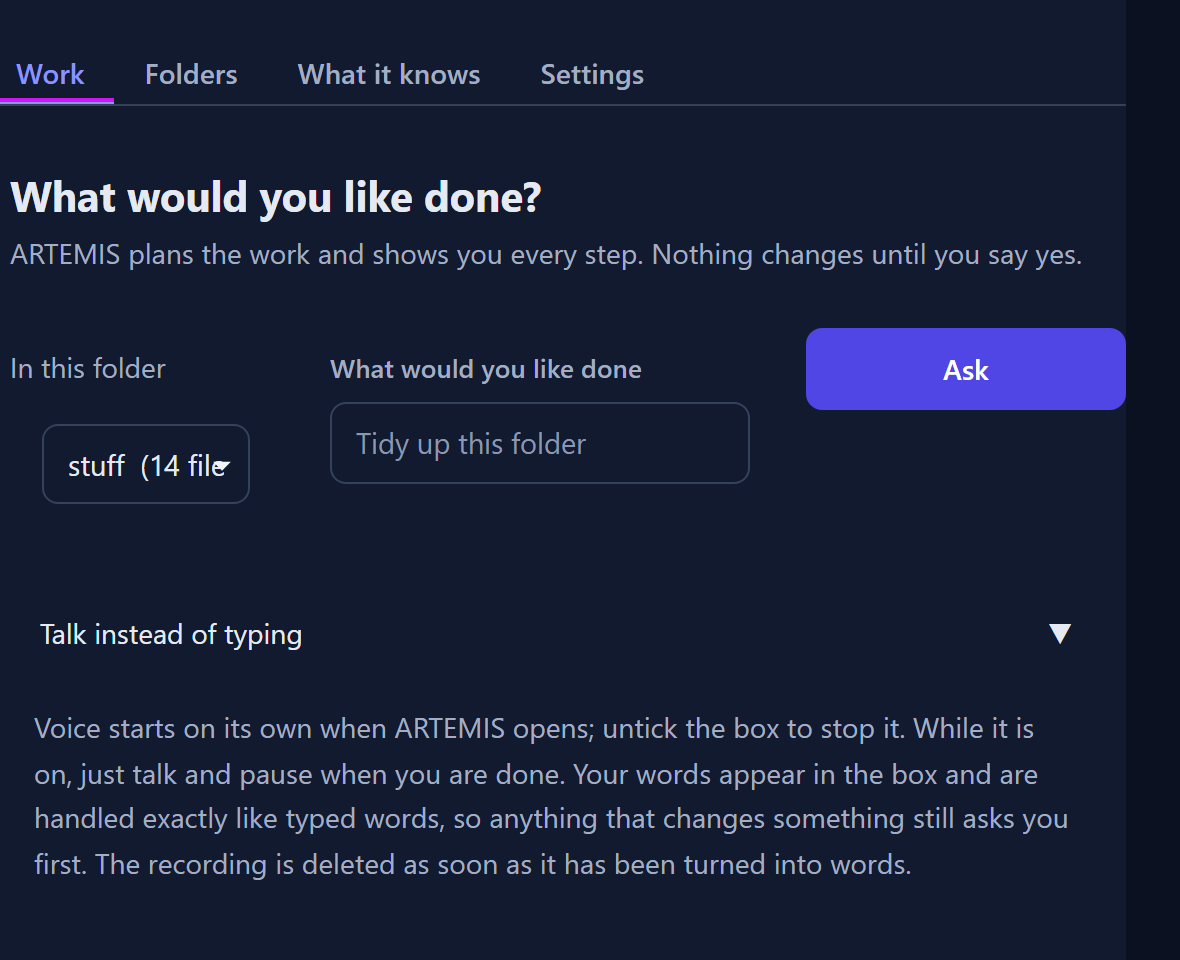
\includegraphics[width=0.64\textwidth]{Figures/s_dark.png}
\caption{The Work screen in the dark theme.}
\label{fig:gui8}
\end{figure}

\section{Database Design}
The system is based on SQLite as its system of record and a per-workspace vector index stored on the filesystem. The relational store is small and highly normalised, and all tables except the workspace table are subordinate to a grant, which is what allows the expression of revocation as a single cascading deletion.

\subsection{ER Diagram}

The workspace entity is the centre of the entity relationship structure. There are numerous indexed files, numerous sessions, numerous memory entries, numerous automation rules, numerous policy rules and numerous undo journal entries and all these relationships are one-to-many identifying relationships with deletion cascading down to the workspace. A session consists of numerous turns, once more cascading. The audit log is explicitly external to this structure: it is a reference to a workspace, but not owned by a workspace, since an audit record of a revoked workspace must outlive that revocation, and a log of its subject can be erased is not an audit log.

This structure articulates two demands. FR-5 is made the cascade, such that the revocation of a grant automatically removes all that is based on it instead of depending on a cleanup routine that may not be complete. FR-18 is the lack of a cascade on the audit log, such that the history of what has happened cannot be erased by deleting its object. The resulting structure is illustrated in Figure~\ref{fig:er}..

\begin{figure}[p]
\centering
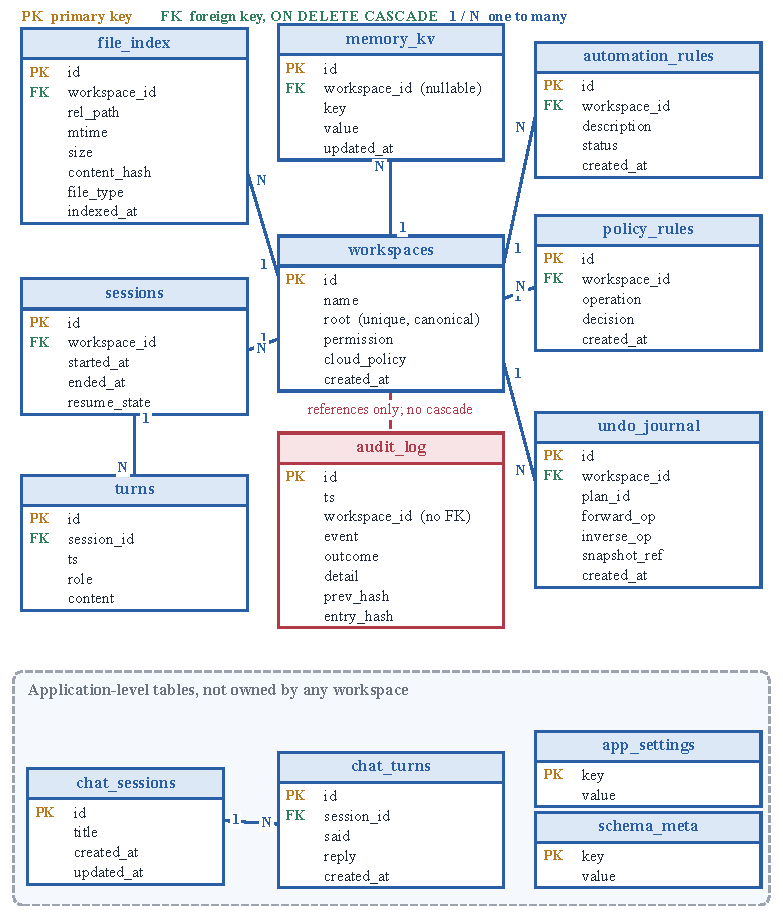
\includegraphics[width=\textwidth]{Figures/fig_er.pdf}
\caption{Entity relationship diagram.}
\label{fig:er}
\end{figure}

\subsection{Data Dictionary}
Table~\ref{tab:datadict} defines each table, its purpose and its principal attributes.

{\small
\Needspace*{7\baselineskip}
\begin{longtable}{|p{2.6cm}|p{4.0cm}|p{6.2cm}|}
\caption{Data dictionary of the relational system of record.}\label{tab:datadict}\\*
\hline
\textbf{Table} & \textbf{Purpose} & \textbf{Principal attributes} \\*
\hline
\endfirsthead
\caption[]{continued from previous page}\\*
\hline
\textbf{Table} & \textbf{Purpose} & \textbf{Principal attributes} \\*
\hline
\endhead
\hline
workspaces & One row per folder the user has granted & id; name; root, stored canonically and unique; permission, being read only or read and write; cloud policy; created at \\
\hline
file\_index & What exists and where, mechanical and rebuildable & id; workspace id; relative path; modification time; size; content hash; file type; indexed at. Unique on workspace and relative path \\
\hline
audit\_log & Append-only, hash-chained record of proposals, refusals and actions & id; timestamp; workspace id; event; outcome; detail; previous hash; entry hash \\
\hline
sessions & Session lifecycle and resume state & id; workspace id; started at; ended at; resume state \\
\hline
turns & Conversation history within a session & id; session id; timestamp; role; content \\
\hline
memory\_kv & Interpretive long-term memory: preferences, facts, named entities & id; workspace id; key; value; updated at. Unique on workspace and key \\
\hline
automation\_rules & Proposals and accepted rules from repeated task detection & id; workspace id; description; status, being proposed or accepted; created at \\
\hline
policy\_rules & User-configured approval preferences, scoped to one operation in one workspace & id; workspace id; operation; decision; created at \\
\hline
undo\_journal & Forward and inverse operations with snapshot references & id; workspace id; plan id; forward operation; inverse operation; snapshot reference; created at \\
\hline
\end{longtable}
}

The trust claim and merit explicit statement are carried by two design points in this schema. Referential integrity should be turned on all connections, as the database engine defaults it off and the cascade clauses would otherwise be silently ineffective, which would result in revocation leaving data behind and seemingly succeed. The hash chain of the audit log connects one entry to the previous one, such that any attempt to modify or delete an entry disrupts the chain and the integrity of the record can be checked instead of being presumed.

In addition to the relational store, every workspace has its own vector index in a different directory. This seclusion is intentional. It implies that the embeddings of a workspace cannot be accessed when another workspace is open even in the case of a query defect, as the index is not open, and it makes workspace revocation a deletion of a directory. Snapshots of content are stored in a common blob store, such that duplicate snapshots of a file that has not changed are free.

\section{Risk Analysis}
Table~\ref{tab:risks} identifies the principal risks to the project, assessing each for likelihood and impact and stating its mitigation.

{\small
\Needspace*{7\baselineskip}
\begin{longtable}{|p{0.8cm}|p{3.6cm}|p{1.3cm}|p{1.3cm}|p{5.0cm}|}
\caption{Project risks.}\label{tab:risks}\\*
\hline
\textbf{ID} & \textbf{Risk} & \textbf{Likeli-hood} & \textbf{Impact} & \textbf{Mitigation} \\*
\hline
\endfirsthead
\caption[]{continued from previous page}\\*
\hline
\textbf{ID} & \textbf{Risk} & \textbf{Likeli-hood} & \textbf{Impact} & \textbf{Mitigation} \\*
\hline
\endhead
\hline
R-1 & A local model small enough for a student laptop proves inadequate for the planning tasks & Medium & High & Bounded failover to a cloud tier under per-workspace opt-in; capability probing in the router; degradation to a stated limitation rather than an error \\
\hline
R-2 & Approval fatigue erodes the safety benefit the gates provide & High & Medium & Configurable granularity and scoped remembered approvals; outward gates remain fixed; the evaluation tests for fatigue directly rather than assuming its absence \\
\hline
R-3 & A confinement defect permits access outside a grant & Low & Critical & Resolution confined to one component; canonicalisation before containment; adversarial tests for traversal, symbolic links, absolute paths and name-prefix siblings \\
\hline
R-4 & Synthesised text contains unsupported claims & High & Medium & Citation map carried through to the answer; unsupported claims rendered as such; a faithfulness check is identified as an open gap rather than claimed as solved \\
\hline
R-5 & Prompt injection from an adversarial document causes an unintended action & Medium & High & Provenance tagging; a structured plan as the interface; policy evaluated out of band; user preview of outward actions; blast radius bounded by the workspace \\
\hline
R-6 & Index growth degrades retrieval or rebuild time & Medium & Medium & Per-workspace indexes; incremental re-embedding by content hash; two-stage retrieval; configurable ceilings \\
\hline
R-7 & The scope proves too large for three members across two semesters & Medium & High & Staged build order with the boundary and gates first; the remote plane is optional by construction and may be dropped without affecting the rest \\
\hline
R-8 & The audience perceives no differentiation from existing assistants & Medium & Medium & Bounded workspace and local-first operation stated explicitly in the product; the disclosure panel makes the claim falsifiable \\
\hline
R-9 & Evaluation participants are drawn from one institution, limiting generalisability & High & Low & Stated as a limitation; segment analysis reported; conclusions framed to the studied population \\
\hline
R-10 & Undo fails to restore state after a partially completed plan & Low & High & Snapshots recorded before mutation; reversal in reverse order; irreversible steps reported rather than silently skipped \\
\hline
\end{longtable}
}


\section{Conclusion}
This chapter has defined what the system should do and in what circumstances. It enumerated the features and 35 functional requirements, each of which is formulated in a manner that it can be verified, the quality attributes and nonfunctional requirements, the assumptions, four use cases that test the key architectural components, the hardware and software requirements, the interface, the database design and the major risks. The specification provides the verification criteria that Chapter 7 applies to its test cases and Chapter 9 applies to the prototype. The next chapter describes the approach by which these requirements are realised.

\chapter{Proposed Approach and Methodology}
This chapter explains how the specification of Chapter 4 is realised and how the project is carried out. It declares the overall architectural plan and the rationale of the plan, gives the procedural detail of the mechanisms that control the behaviour of the system, outlines the development methodology and the sequence of building, and outlines the evaluation methodology. The focus is on the rationale and the processes and not on the implementation detail, which is in Chapter 6.

\section{Overall Approach}
The method is based on one proposition, on which all the structural decisions in this project are based: the limitation of the scope of the assistant should be structural and not behavioural. It should be impossible by design and not discouraged by teaching.

The difference is consequential. A system that instructs a model not to access material outside a workspace has expressed a preference, and that preference can be defeated by a sufficiently persuasive document, an unanticipated phrasing, or a defect in the model's compliance. A system where no other component than a single broker can transform a reference into a filesystem path, and where that broker determines the path to its actual location and then checks containment has asserted an invariant. The former can be argued past, the latter cannot, since there is no code path along which the argument can run.

This suggestion is repeated thrice, which results in the three mechanisms that characterize the system.

The initial use is confinement. All path resolution is directed through a single component, canonicalised and then containment is tested. This is what makes the difference between a boundary and a suggestion, since a path with a traversal segment or a symbolic link to the outside of the grant is solved to its real position prior to the test being run. To undo these two steps would be to accept a course which only seemed to be enclosed.

The second use is the denial of destruction. Instead of putting destructive operations behind a confirmation, the system offers no operation that does one. No deletion approval dialogue exists since there is no deletion code path. A policy is a gate that the user can click through; an architecture is a gate that does not exist. It is what allows the assertion that the system deletes nothing is a property of the system and not a promise concerning the behaviour of a model.

The third use is the separation of proposal and execution. The planner creates a plan and is unable to implement it. The dispatcher performs and is unable to plan. The policy engine between them makes a decision on every proposed call, and the dispatcher rejects any call whose decision is not present or does not match it. It is this separation that renders prompt injection a constrained problem: text in a document cannot be an authorised instruction, since an instruction must be a well-formed declaration that has passed an out-of-band policy check, and no quantity of persuasive prose can generate one.

\section{The Risk Classification Procedure}
The policy engine categorizes each proposed call into precisely one of four levels. The system has a major decision mechanism, the classification procedure, and its properties are not accidental.

The order of evaluation is predetermined, and denials are considered prior to permissions. Every rule is returned immediately, and thus the decision is the first rule to give what a subsequent rule cannot give. The order is as follows.

\begin{enumerate}
    \item 1. If any path the call touches lies outside the active grant, deny it as destructive
    \item 2. If the operation is itself destructive, deny it
    \item 3. If the operation leaves the machine, gate it, and do so regardless of configuration
    \item 4. If the operation changes state, gate it unless the user has recorded a rule permitting that operation in that workspace
    \item 5. If the operation is a recognised read, allow it
    \item 6. Otherwise deny it, because an unrecognised operation is treated as unknown rather than as harmless
\end{enumerate}

The final rule warrants comment. An operation the system does not recognise is refused rather than permitted, because silently permitting unrecognised operations is the mechanism by which a boundary erodes over time. A system that defaults to permission accumulates capability it was never designed to have.

The containment test within the first rule is delegated to the broker rather than reimplemented. This is deliberate: it ensures that exactly one containment check exists in the system, rather than two that may drift apart as the code changes.

Table~\ref{tab:tiers} states the four tiers, their default treatment and their recoverability.

{\Needspace*{3\baselineskip}
\begin{longtable}{|p{2.4cm}|p{4.6cm}|p{3.4cm}|p{3.0cm}|}
\caption{The four risk tiers.}\label{tab:tiers}\\*
\hline
\textbf{Tier} & \textbf{Definition} & \textbf{Default} & \textbf{Recovery} \\*
\hline
\endfirsthead
\caption[]{continued from previous page}\\*
\hline
\textbf{Tier} & \textbf{Definition} & \textbf{Default} & \textbf{Recovery} \\*
\hline
\endhead
\hline
T0 Read & Reads within the granted workspace. No change, no egress. & Executes automatically & Not applicable \\
\hline
T1 Reversible & Changes workspace state and is fully invertible from a snapshot. & Configurable: automatic, batch approval, or per action & Full \\
\hline
T2 Outward & Leaves the machine: mail, web request, cloud model call carrying workspace content. & Always gated. Not configurable. & Partial; logged, and recallable only where the protocol permits \\
\hline
T3 Destructive & Deletion, overwriting without a snapshot, writing outside the workspace. & Refused. Not gated, because structurally unavailable. & Not applicable \\
\hline
\end{longtable}
}

The adjustable level is T1 in isolation and this is how the research discovery in Chapter 2 is respected. Since the respondents were almost evenly split on whether an assistant should seek permission before taking action, approval granularity is a setting and not a choice. An approval remembered is limited to a single operation in a single workspace, such that approval of a folder tidy does not grant permission to send mail, and the engine will not remember such a rule to an outward or destructive operation regardless of what is requested.

\section{The Recovery Procedure}
Two procedural rules govern recovery, each of which deals with a common failure mode of undo mechanisms.

The snapshot is taken prior to the mutation, never after. The inverse is recorded post facto, and the state that the operation has already created is reversed to nothing. Each route through the journal thus writes its entry and only then allows the caller to act.

The strategy is selected by cost. A tiny file is replicated into a content-addressed store, such that successive snapshots of an identical file incur no extra cost than the initial. A big file is hard-linked where the filesystem allows it. A relocation or renaming does not involve any copying of content whatsoever, as its reverse is purely structural. A deletion record is sufficient to create a new file.

Reversal is at the granularity of the plan and not the individual operation. A reverse of a folder tidy undoes all the moves of the folder in reverse order since the plan is the unit that the user was requested to approve. It needs to be reversed, not cosmetic: a program that builds a directory and then transfers files into it must transfer the files out of it before the directory can be deleted. A step that cannot be undone is not re-raised as an error, and thus one bad file does not leave the rest of the reversals behind.

\section{The Prompt Injection Defence}
The system reads documents, source code and web results, all of which can be manipulated by an adversary, and the security literature examined in Chapter 3 recognizes this as the main threat to an agentic system. It is not a detection approach, which is unreliable, but the structural impossibility of retrieved content becoming an authorised instruction. There are five independent defences, each of which is adequate on its own..

\begin{itemize}
    \item Each context chunk is marked with its provenance user, workspace file, web or tool result, and only user chunks can be the source of an intent. All others are treated as data
    \item The planner emits a structured plan rather than prose, so a tool call must be a well-formed declaration and text within a document cannot become one by being persuasive
    \item The policy engine does not read the reasoning text of the model, only the tool call, and therefore nothing in a document can change a verdict.
    \item Each outward action gives the user a tangible preview of what will happen, recipient and content, and thus an attempted exfiltration must pass through a person reading it in plain text.
    \item The workspace boundary restricts the effects of a completely successful injection to a single granted workspace, and no deletion or egress outside the policy of that workspace.
\end{itemize}

The final defence is the strongest argument for the bounded-scope hypothesis, because it bounds the worst case rather than only the expected case.

\section{Development Methods}
The project is developed in an incremental and iterative approach structured into two-week sprints, and the backlog is represented in the form of user stories with Fibonacci point estimates. Every sprint provides a single step in the build sequence and ends with a stage gate, a test that must pass before the stage is declared complete. A stage is not delivered because its code is; it is delivered because its gate is passed.

The decision to use an incremental approach is based on the risk profile of the project and not preference. The main danger is that the trust machinery is impossible to retrofit when features rely on it, and the approach taken is to build that machinery first and test it on inert tools before any model is engaged.

There were two other approaches. A waterfall approach was dismissed since the specification relies on discoveries that can only be made during construction, including whether a local model of workable size can plan sufficiently. An entirely feature-based model, constructing the visible capabilities and then adding protection later, was dismissed on the more compelling ground: the boundary and the gates are the very elements that cannot be added afterwards, since all the features constructed before them would have to be rewritten to traverse them.

The build sequence is shown in Table~\ref{tab:build}. Its ordering is a single principle, that a property must exist before anything can be demanded to possess it.. The boundary must exist before anything the workspace broker, the file can be bounded. watcher and the disclosure panel.

{\Needspace*{7\baselineskip}
\begin{longtable}{|p{1.2cm}|p{5.6cm}|p{6.4cm}|}
\caption{The build sequence.}\label{tab:build}\\*
\hline
\textbf{Stage} & \textbf{Deliverable} & \textbf{Reason for this position} \\*
\hline
\endfirsthead
\caption[]{continued from previous page}\\*
\hline
\textbf{Stage} & \textbf{Deliverable} & \textbf{Reason for this position} \\*
\hline
\endhead
\hline
1 & Workspace foundation: the store, the workspace broker, the file watcher and the disclosure panel. No model involved. & The boundary must exist before anything can be bounded. \\
\hline
2 & Policy engine, approval broker and undo journal, exercised against placeholder tools. & Inexpensive now and near-impossible to retrofit; provable before any model introduces non-determinism. \\
\hline
3 & The gateway: model router, context engine, agent planner and tool dispatcher. & The highest-risk stage, validated against gates that already function. \\
\hline
4 & Session resume, folder tidy and repeated task detection. & The first real capabilities, exercising the read and reversible tiers end to end. \\
\hline
5 & Notes synthesis and code assistance, with the index, retrieval and citation map. & Introduces the vector index only once the boundary is proven. \\
\hline
6 & Web search, mail composition and document drafting. & The first outward actions, permitted only after the gates are demonstrated. \\
\hline
7 & Speech input and output over the existing turn normaliser. & Should require no new gate. If it does, the interaction layer was designed wrongly, so this stage tests the parity claim. \\
\hline
8 & Remote access plane. & Genuinely optional; a complete product exists without it. \\
\hline
\end{longtable}
}

The most consequential decision in this sequence is the placement of stage 2 before the model work. It implies that the trust machinery can be tested, and proved, prior to any model non-determinism being introduced into the system. A defective gate at that point is a deterministic defect with a short reproduction, which is no longer true when a model is producing the plans.

The stage 7 gate is of special interest since it is designed to fail. The assertion that voice is parity by construction is challenged by the fact that the speech stage must not add a new approval gate. In case a new gate was needed, the assertion would be incorrect and the interaction layer would require redesign. A gate that fails no tests.

\section{Evaluation Methodology}
The assessment, which is performed in the second stage of the project, is a test of the central hypothesis and the constraints that the literature review found to be inherited. It consists of four elements.

Task-based measurement involves comparing the participants who complete representative multi-file tasks with and without the system, and the time and success rate of completion. The cognitive workload is assessed with a developed subjective measure that is given at the end of each task. The measurement of usability and trust is by questionnaire, and trust is instrumented against the bounded- scope claim, such that the hypothesis is tested and not assumed.

Three other tests deal directly with the inherited limitations, since the literature suggests that each would otherwise be asserted rather than proved. Approval fatigue is not tested in a single session, but in repeated sessions, as it cannot be observed in a single session. Synthesis faithfulness and citation accuracy are quantified wherever source metadata allows, and any deficiency is reported as a known limitation. Code assistance is checked to ensure that no change is ever made without express permission and that no previous user edit is overwritten without notice.

At the end of the first phase the parts of this methodology that do not require participants were carried out and are reported in Chapter 9, and the parts that do are planned for the second phase and are listed in Chapter 10.

The voice assessment is based on the design advice provided in the literature. It sets a target of four seconds latency threshold, natural spoken fillers instead of tones during waiting times, and reports cognitive workload and trust and task time and success, as the reviews determined that standard usability measures do not capture these voice-specific issues.


\section{Conclusion}
The approach and the methodology have been outlined in this chapter. It said the plan of laying the guarantees in structure, provided the steps to classify the risks, recover and the defence against prompt injection, explained the incremental approach and the build sequence where each step has to pass its gate before the next one starts and the evaluation. The steps outlined here are the steps that the implementation takes and the evaluation tests. The next chapter presents the design that realises them.

\chapter{High-Level and Low-Level Design}
This chapter presents the design of the system. It begins with an overview and the considerations that constrain the design, then presents the architecture at the layer and component level, the strategies that produced it, the domain model, and the policies and tactics that govern implementation. Diagrams are provided throughout, and each significant decision is traced to the requirement or finding that produced it.

\section{System Overview}
The system is a long-running local process that mediates between a user and a bounded region of their filesystem. It accepts a request by typing or by speech, retrieves context from within the granted workspace, produces a multi-step plan, classifies each step by risk, obtains the user's approval where required, records how to reverse each change, executes the approved steps, and writes an immutable record of everything proposed and performed.

The design is organised as six layers on the execution path with two planes crossing all of them, as shown in Figure~\ref{fig:layers}. The presentation layer provides the command line, graphical and optional remote surfaces over one shared view model. The interaction layer normalises voice and text into a single modalityneutral object. The gateway layer routes model requests, assembles context, classifies risk, plans, and dispatches. The capability layer implements the features. The data layer persists everything locally. The remote access layer is drawn outside the stack because nothing in the layers beneath it depends on its presence.


Layers one to five form the local execution path, the two planes cross every layer, and the remote access plane is drawn outside the stack because removing it leaves a fully functional system.

Security and performance are represented as planes rather than layers, and this is a deliberate representational choice. A layer is a stage a request passes through, and drawing security as a layer would imply that a request could be past security, which is precisely the reasoning error that produces confuseddeputy defects. They are drawn as planes to indicate that every arrow in the architecture crosses both.


\section{Design Considerations}
\subsection{Assumptions and Dependencies}
The design depends on the following, each of which would require reconsideration were it to change.

\begin{itemize}
    \item The canonicalisation procedure of the operating system solves symbolic links in the right way, as the confinement guarantee is constructed on the basis of it. This is all the platform-specific behaviour on which the design relies.
    \item The relational store maintains referential integrity where it is asked to, as revocation is defined as a cascading deletion. Since the engine switches this off by default, it would need to be turned on in each connection.
    \item There is a local model runtime or the user has set up cloud fallback on the workspaces in question. Providers are considered configuration by the router and thus provider change is not design change.
    \item The user is a single person who has control over the folders he/she grants. The design does not deal with shared or simultaneous access by more than one user.
    \item The design thus views all the content retrieved as data and not instruction.
    \item The capability layer is likely to see the biggest change in functionality since they are added. The reason why the uniform tool contract exists is that the change does not spread to the gateway.
\end{itemize}

\subsection{General Constraints}
The design was influenced by the following constraints and the effect of each is mentioned.

\begin{itemize}
    \item \textbf{Resource envelope.} The system should be usable on a consumer laptop, which entails the expensive work is asynchronous and all the queues are limited. The execution plane in Section 6.4 is the result of impact.
    \item \textbf{Offline operation.} Connectivity should never be part of core functionality, which demands that a local model should be the default tier, and that networked capabilities degrade explicitly. The impact is the degradation contract in Table~\ref{tab:degradation}
    \item \textbf{Data residency.} The data of the users should not be sent to a server operated by the project, so the egress is enforced in the router, where workspace policy is known, but not in the tool layer.
    \item \textbf{No inbound port.} The remote aircraft needs to make an outward dialing hence a topology in Section.
    \item \textbf{Credential handling.} The secrets should be stored in the operating system keyring, which is not part of the system storage tree itself and not backing up of the system.
    \item \textbf{Verification.} All the guarantees should be testable and this demands that they have a single point of enforcement. This is why there is resolution in one aspect and execution in the other.
    \item \textbf{Team and timeline.} The architecturally detachable plane is necessitated by the need to have the optional components separable by three members in two semesters.
\end{itemize}

\subsection{Goals and Guidelines}
The design is dominated by four principles and the purpose behind them is mentioned since none of them is self-explanatory.

A house should be built and not advertised. Where it is possible to express a guarantee in terms of the non-existence of a code path, it is expressed in that form. This is the reason why devastating operations are not discussed as to their approval: a defect can defeat a check or a defective route or an unexpected turn, but an incapacity cannot.

\begin{figure}[tbp]
    \centering
    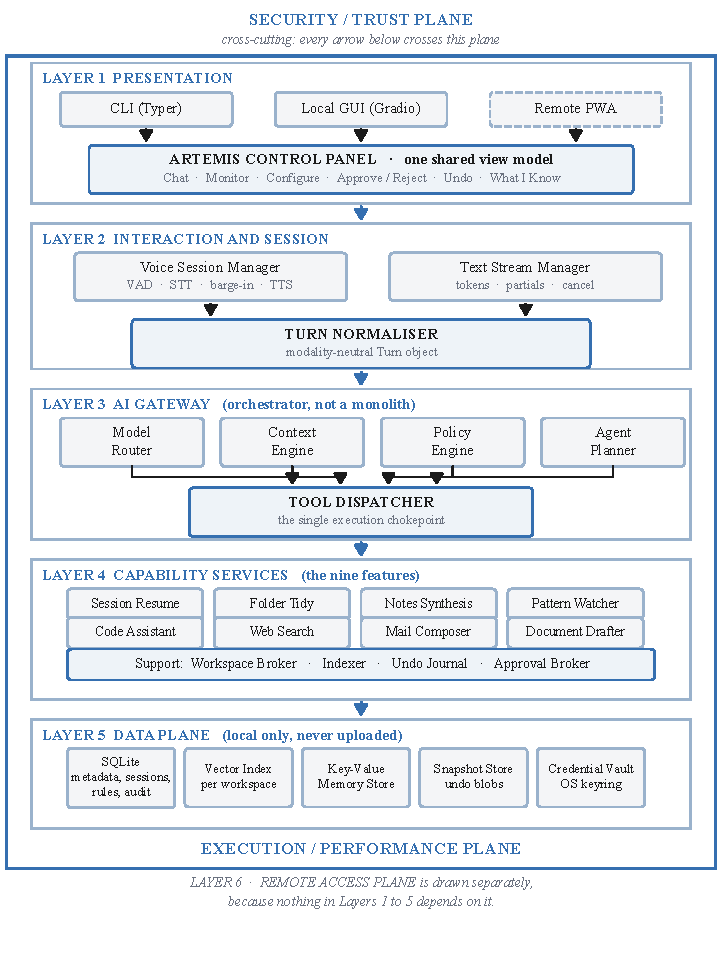
\includegraphics[width=\textwidth]{Figures/fig_layers.pdf}
    \caption{The layered architecture.}
    \label{fig:layers}
\end{figure}

There are only one enforcement points per guarantee. Resolution is done in the broker and execution in the dispatcher and not in any other place. This is because of verification: a two-point guarantee is one that has two chances to move apart, and no specific point where it can be verified.

Legibility is a component of trust. Background work reports should be visible, cancellable, the disclosure panel is a live query, and not a written summary, and refusals are recorded in the audit log, in addition to actions. This is because a system the behaviour of which cannot be observed cannot be trusted no matter how correct it turns out to be.

The refusal failure mode occurs. An operation that has not been recognised is denied, an unsolvable path is rejected, a queue that has reached its full length throws off work into view and an expired approval will never execute. This is because any failure that is not prohibited by a system containing a boundary transforms a defect into a breach.

\subsection{Development Methods}
Design was generated by generating structure based on research results and specification as opposed to modifying a reference architecture. The layered structure with cross-cutting planes is traditional, and the decomposition of the components inside the gateway is due to a particular need: the initial design left routing, context, memory, planning, policy and dispatch to the same component, and this was not testable since no single guarantee could be isolated. The four component decomposition with one common execution point was taken to ensure that each guarantee becomes verifiable. This revision also added the policy engine, as a first-class component, transforming the approval-first finding into enforced structure..

\section{System Architecture}
The system's responsibilities are partitioned so that each guarantee is held by exactly one component. Table~\ref{tab:components} presents the component inventory, stating for each component its layer, its responsibility and the single thing it must never do. The final column is the operative one: it states the invariant whose violation would constitute a defect in the architecture rather than in the implementation.

{\small
\Needspace*{12\baselineskip}
\begin{longtable}{|p{0.6cm}|p{2.8cm}|p{0.9cm}|p{4.0cm}|p{4.2cm}|}
\caption{Component inventory.}\label{tab:components}\\*
\hline
\textbf{\#} & \textbf{Component} & \textbf{Layer} & \textbf{Responsibility} & \textbf{Must never} \\*
\hline
\endfirsthead
\caption[]{continued from previous page}\\*
\hline
\textbf{\#} & \textbf{Component} & \textbf{Layer} & \textbf{Responsibility} & \textbf{Must never} \\*
\hline
\endhead
\hline
1 & Command line interface & 1 & Scriptable control surface & Bypass the approval broker \\
\hline
2 & Graphical control panel & 1 & Visual control surface, loopback-bound & Bind to a non-loopback interface \\
\hline
3 & Control panel view model & 1 & Single source of interface truth across surfaces & Hold state the backend does not own \\
\hline
4 & Voice session manager & 2 & Activity detection, transcription, interruption, synthesis & Record when not explicitly armed \\
\hline
5 & Text stream manager & 2 & Token streaming and cancellation & Buffer past a cancellation \\
\hline
6 & Turn normaliser & 2 & Produce the modality-neutral turn & Leak modality downstream \\
\hline
7 & Model router & 3 & Select a tier and fail over; enforce egress & Send workspace data to a disabled tier \\
\hline
8 & Context engine & 3 & Assemble bounded, cited context & Include content outside the grant \\
\hline
9 & Policy engine & 3 & Classify risk and decide gating & Be consulted after execution \\
\hline
10 & Agent planner & 3 & Produce a multi-step plan & Execute anything itself \\
\hline
11 & Tool dispatcher & 3 & Sole execution point & Accept a call lacking a policy verdict \\
\hline
12 & Capability services & 4 & The features & Touch the filesystem directly \\
\hline
13 & Workspace broker & 4 & Path resolution and confinement & Resolve a path outside a grant \\
\hline
14 & Indexer & 4 & Incremental indexing and embedding & Block the interactive path \\
\hline
15 & Undo journal & 4 & Snapshots and inverse operations & Record an action after the fact \\
\hline
16 & Approval broker & 4 & Hold pending actions and fan out to surfaces & Approve on timeout \\
\hline
17 & Data plane stores & 5 & Local persistence & Serialise outside the host \\
\hline
18 & Remote access plane & 6 & Authenticated relay & Store or read plaintext user data \\
\hline
\end{longtable}
}

The collaboration between these components is expressed by the request lifecycle shown in Figure~\ref{fig:lifecycle}, which is the single most important path in the system. Every request, whether spoken or typed and whether local or remote, traverses exactly this sequence, and no shortcut exists.

\begin{figure}[H]
    \centering
    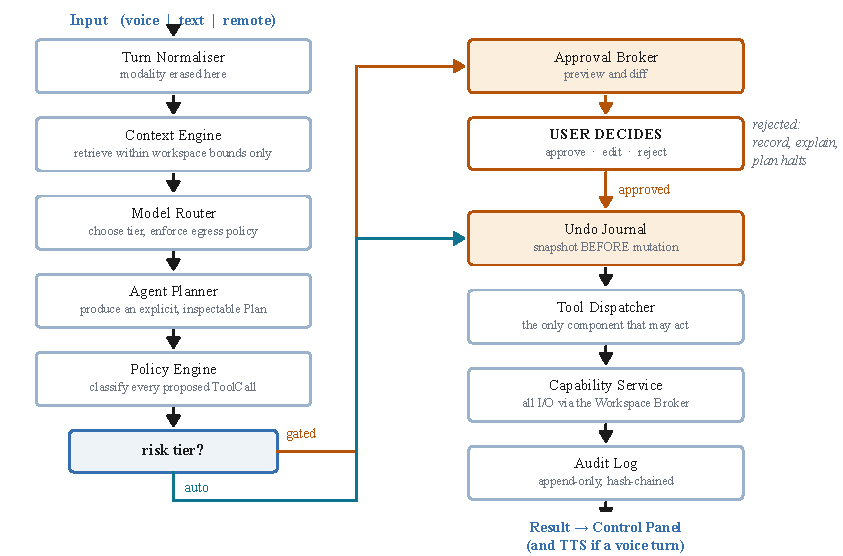
\includegraphics[width=\textwidth]{Figures/fig_lifecycle.pdf}
    \caption{The request lifecycle.}
    \label{fig:lifecycle}
\end{figure}

The turn normaliser erases modality, policy engine is consulted by the dispatcher, the snapshot comes before the mutation, and audit entry is written regardless of whether action is taken or rejected.

This path has five invariants that are imposed and collectively they make up the guarantees of the architecture. The dispatcher consults the policy engine but never after. The undo journal captures the snapshot of the undo journal prior to the mutation, but never afterwards. Even in the case of action being rejected, the audit entry will be written and therefore the log will capture what was proposed and not just what happened. A call without a corresponding policy verdict is refused by the dispatcher. Voice and text turns are no different than the planner on and that is what makes voice parity structural and not a second implementation.

The decomposition was chosen over two alternatives. One orchestrating component was abandoned due to the impossibility of isolating any single guarantee to be tested, and the fact that a flaw in one component would invalidate all the guarantees at the same time. An arrangement, where each capability had its own gating logic, was not accepted as it would create as many points of enforcement as features, none of which could be centrally audited, and none of which could drift.

\subsection{Subsystem Architecture: The Gateway}
In Figure~\ref{fig:gateway}, the gateway is broken into four parts having one common point of execution. The planner generates a plan and cannot implement it; the dispatcher implements and cannot generate plans; the policy engine decides on a per-proposed-call basis whether a particular model tier can be used and whether data can leave the machine; and the router decides whether a particular model tier can be used and whether data can leave the machine.

\begin{figure}[tbp]
    \centering
    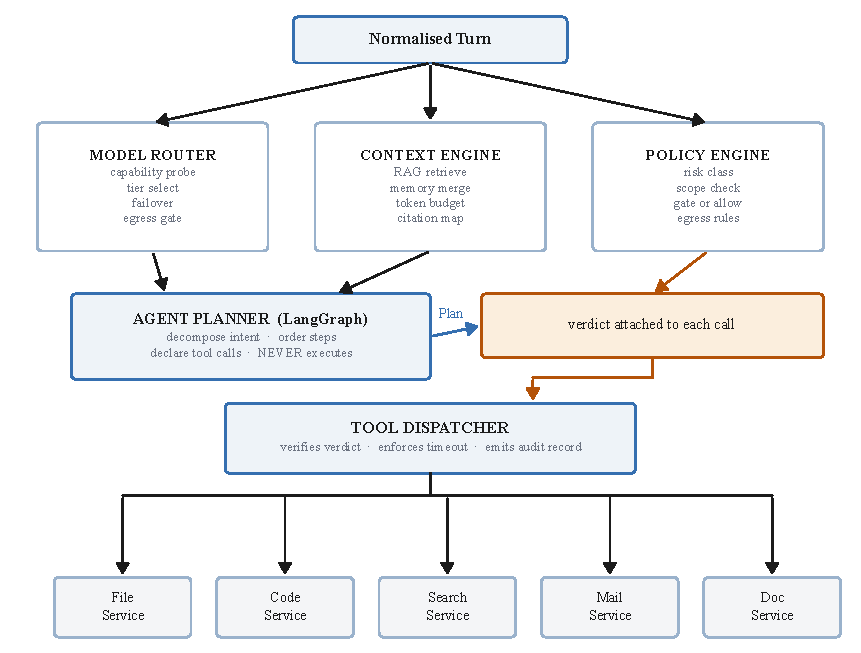
\includegraphics[width=\textwidth]{Figures/fig_gateway.pdf}
    \caption{Internal structure of the gateway.}
    \label{fig:gateway}
\end{figure}

The planner comes up with a plan but never implements it and all the calls end up at the dispatcher, the only point of execution..

The model router is the owner of tier selection and egress enforcement. The reason why egress is applied here and not in the tool layer or the prompt is that the router is aware of the cloud policy of a particular workspace. The default is the tier zero which is the local model. Later levels can only be accessed where the workspace allows, and any readable endpoint can be added as a new level without any alteration to the code as the providers are considered as configuration, but not as branches. The max retries per tier are defined as one, and only after that do you continue to the next tier, meaning that a workspace that is cloud disabled has only one tier and its failure yields a clean degradation message instead of an undefinite wait. The selection and the egress gate are indicated in Figure~\ref{fig:router}.


Higher levels are only accessible in the cases where the cloud policy of the workspace allows and all egress is logged.

\begin{figure}[tbp]
    \centering
    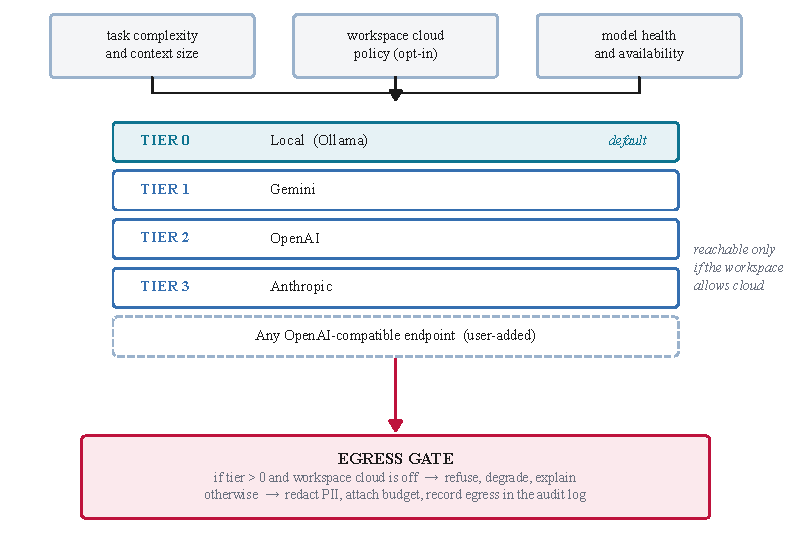
\includegraphics[width=\textwidth]{Figures/fig_router.pdf}
    \caption{Tier selection and the egress gate.}
    \label{fig:router}
\end{figure}

The context engine assembles the working context of the model, and imposes limited scope on the read side, just as the broker does on the write side. Each retrieved chunk is identified by the identifier of the workspace where it was retrieved and any chunk which does not match the active grant is discarded and the discard is recorded. The token budgeter is recency-relevant and never truncates a citation source in silence. Each chunk is stored back to the file and line, in the form of a citation map, and it is this map that makes the synthesis feature verifiable, as a claim that can not be traced by the map is reported as unsupported and not as established. This assembly is depicted in Figure~\ref{fig:context}..


The retrieved chunks all bear a workspace identifier, any chunk not within the active grant is deleted and the discard recorded, and the citation map is taken with to the answer.


The policy engine assigns every proposed call in a procedure as declared in Chapter 5. The four levels and the order of evaluation are shown in Figure~\ref{fig:tiers} and \ref{fig:policyorder} respectively, with denials and gates being earlier than permissions and gates respectively.



The user can only configure the reversible tier, outward actions are always gated and destructive actions are structurally inaccessible.

\begin{figure}[tbp]
    \centering
    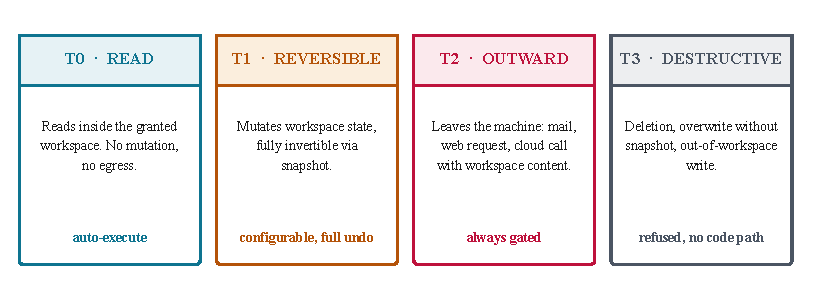
\includegraphics[width=\textwidth]{Figures/fig_tiers.pdf}
    \caption{The four risk tiers.}
    \label{fig:tiers}
\end{figure}

\begin{figure}[tbp]
    \centering
    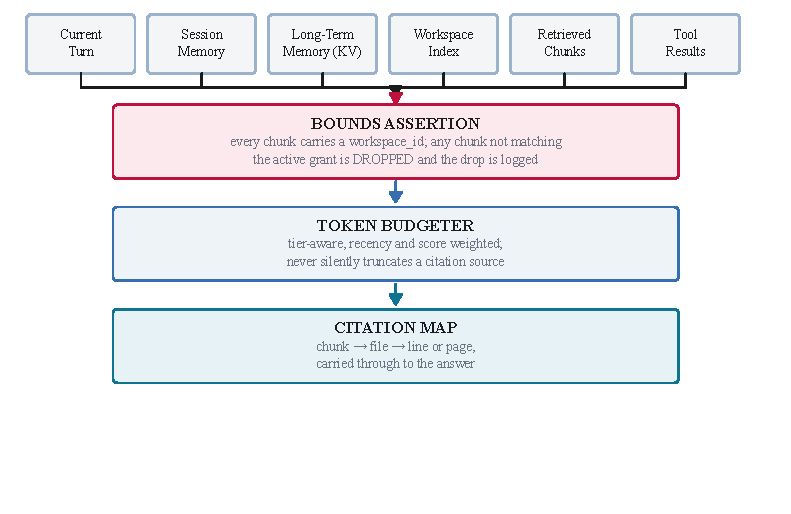
\includegraphics[width=\textwidth]{Figures/fig_context.pdf}
    \caption{Context assembly.}
    \label{fig:context}
\end{figure}


Denials are considered preceding gates and gates preceding permissions to ensure that the first match is the decision and no subsequent rule can grant what a preceding rule denied.


Figure~\ref{fig:approval} displays a worked example of a folder tidy, where the reading steps are automatically executed and the two state-changing steps are gated, resulting in a preview indicating what will happen, and, no less importantly, what will not.

\begin{figure}[tbp]
    \centering
    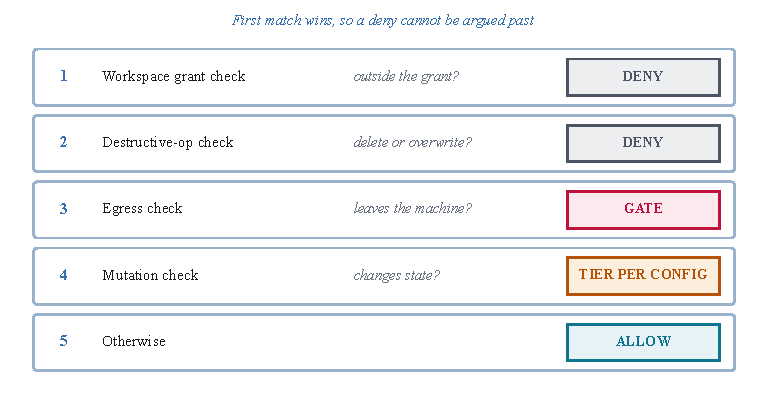
\includegraphics[width=\textwidth]{Figures/fig_policy_order.pdf}
    \caption{Policy evaluation order.}
    \label{fig:policyorder}
\end{figure}

\begin{figure}[tbp]
    \centering
    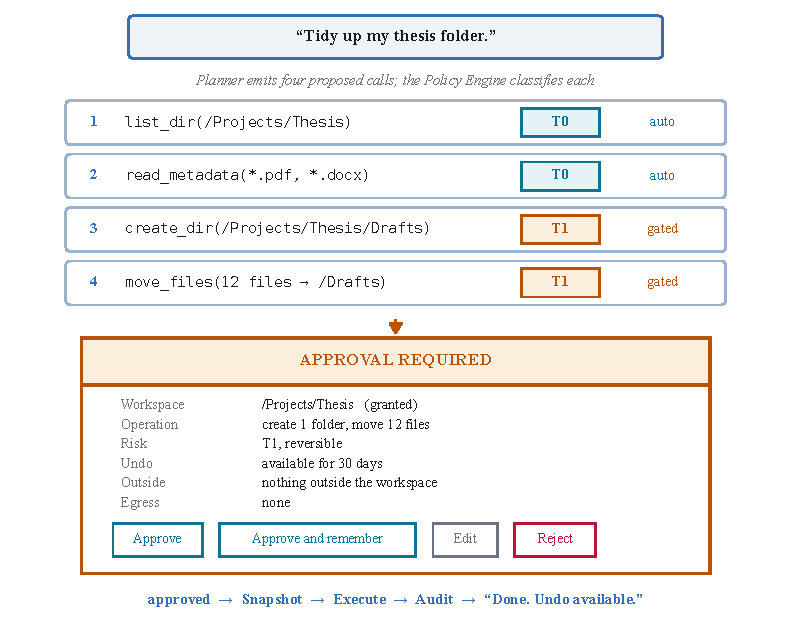
\includegraphics[width=\textwidth]{Figures/fig_approval.pdf}
    \caption{A worked classification for a folder tidy.}
    \label{fig:approval}
\end{figure}

The operations of reading are automatic and the reversible operations are gated, and the preview states that nothing is taken out of the machine and nothing is lost.

The agent planner generates plans based on LangGraph and never performs them. It has an explicit cycle cap and a wall-clock budget that deals with the repetitive-loop failure mode that the planning literature documents: the inability of an agent to converge presents its partial plan and requests (instead of looping forever).

\subsection{Subsystem Architecture: Capability Services}
The features are implemented as services behind a uniform tool contract. None accesses the filesystem, the network or the database itself, but rather accesses them via the common ground of the broker, the. ( journal, the approval broker and the data plane as illustrated in Figure~\ref{fig:services}.

\begin{figure}[tbp]
    \centering
    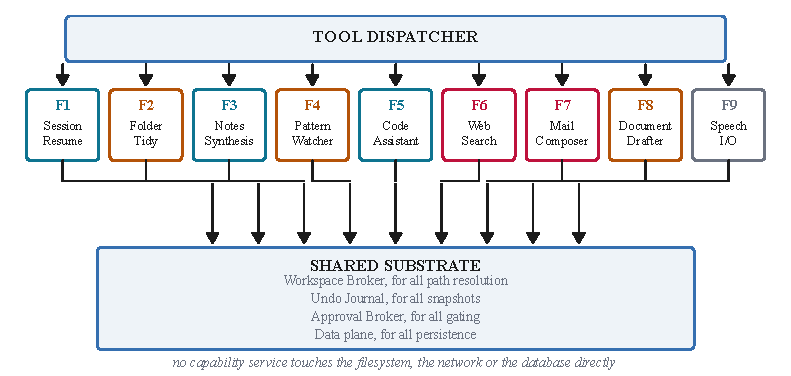
\includegraphics[width=\textwidth]{Figures/fig_services.pdf}
    \caption{Capability services and their access path.}
    \label{fig:services}
\end{figure}

Capability services can only be accessed via the tool dispatcher and only reach the filesystem via the shared substrate, thus no service has its own path to the filesystem.

According to Table~\ref{tab:services}, the upper limit of each service can be requested. The table is a design constraint, not a description: a service cannot demand that it be served at a tier higher than it has stated maximum, which is what limits the impact of a defect in any feature..

{\Needspace*{3\baselineskip}
\begin{longtable}{|p{0.9cm}|p{3.4cm}|p{1.6cm}|p{6.4cm}|}
\caption{Capability services and risk tiers.}\label{tab:services}\\*
\hline
\textbf{\#} & \textbf{Service} & \textbf{Max tier} & \textbf{Notes} \\*
\hline
\endfirsthead
\caption[]{continued from previous page}\\*
\hline
\textbf{\#} & \textbf{Service} & \textbf{Max tier} & \textbf{Notes} \\*
\hline
\endhead
\hline
F1 & Session resume & T0 & Deterministic replay of recorded session state; no model involved \\
\hline
F2 & Folder tidy & T1 & Moves and groups only; no code path to deletion \\
\hline
F3 & Notes synthesis & T0 & Reads and generates; output remains a proposal until the drafter writes it \\
\hline
F4 & Pattern watcher & T1 & Detects three or more repetitions and may only propose a rule; cannot install one \\
\hline
F5 & Code assistant & T0 & Explains and produces a difference; never writes and never executes \\
\hline
F6 & Web search & T2 & On demand only; every query recorded \\
\hline
F7 & Mail composer & T2 & Draft, approve, send; sending is gated regardless of configuration \\
\hline
F8 & Document drafter & T1 & Always writes a new file; never overwrites an existing one \\
\hline
F9 & Speech input and output & Not applicable & Not a service but a modality at layer two, over identical gates \\
\hline
\end{longtable}
}

The fact that the ninth feature is not a service is a structural assertion. Voice is normalised on the interaction layer into the same turn object as text, so it is automatically shared with all approving gate. Parity is obtained thus by construction and not by reimplementing the gates along a second path and the stage seven gate of Chapter 5 is provided to check this.

The logic that transforms a logical reference into a real path is the workspace broker, and Figure~\ref{fig:broker} presents five of its assertions. The second and third place inversion is the whole content of the guarantee: before the test is made, it is necessary to canonicalise a symbolic link or a segment of a traversal to the actual place where it belongs.


Canonicalisation precedes the containment test, of which a boundary and a suggestion differ.


\section{Architectural Strategies}
This section explains the strategies that influenced the architecture, the justification, and the alternatives that were thought of and discarded.

\subsection{Local-First Operation with Optional Egress}
The system is configured to use a local model, and cloud access is an opt-in per-workspace. The logic is tri-fold: the study documented local-first as the most popular deployment choice, privacy emerged as a risk of churn and a reoccurring free-text issue, and offline operation is a known limitation.

The other option of cloud-first functioning and a local backup was discarded as it reverses the guarantee. According to that arrangement the default behaviour is transmitting user data and the user has to take some action to avoid it, but according to the chosen arrangement the user has to take some action in order to allow it. The accepted trade-off is capability: a small local model is not as well as a large hosted model, which is alleviated through limited failover. where the workspace permits and by honest degradation where it does not.

\begin{figure}[tbp]
    \centering
    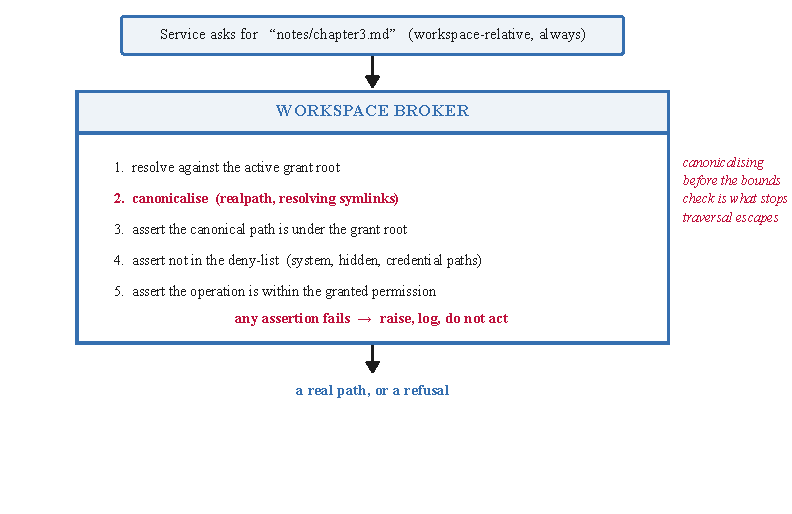
\includegraphics[width=\textwidth]{Figures/fig_broker.pdf}
    \caption{Path resolution and confinement.}
    \label{fig:broker}
\end{figure}

The degradation contract in Table~\ref{tab:degradation} states the required behaviour as each external capability is withdrawn. Each row is a testable acceptance criterion rather than an aspiration, and together they define the system's correctness under adverse conditions.

{\small
\Needspace*{12\baselineskip}
\begin{longtable}{|p{4.6cm}|p{8.6cm}|}
\caption{The degradation contract.}\label{tab:degradation}\\*
\hline
\textbf{Withdrawn capability} & \textbf{Required behaviour} \\*
\hline
\endfirsthead
\caption[]{continued from previous page}\\*
\hline
\textbf{Withdrawn capability} & \textbf{Required behaviour} \\*
\hline
\endhead
\hline
Internet connectivity & Full local operation continues. Cloud model calls, web search and mail sending are disabled, each failing as an explicit retryable action rather than being silently dropped \\
\hline
All cloud model providers & Falls back to the local model. Features exceeding local capability degrade to a stated limitation rather than an error \\
\hline
Local model & Falls forward to the cloud chain, if and only if the workspace permits cloud access \\
\hline
Remote device & The host continues uninterrupted. Approvals in flight revert to pending and appear on the host surface \\
\hline
Remote edge & Local operation is entirely unaffected, because the remote plane is not on the execution path \\
\hline
Workspace grant & The system cannot see the folder. Not declines to touch it: the path is not resolvable at all \\
\hline
\end{longtable}
}

\subsection{Separation of Memory from the File Index}
The system supports two types of knowledge and muddling the two is the fallacy that transforms a limited assistant into a spy device. Figure~\ref{fig:memory} illustrates the five types of memory and Figure~\ref{fig:memoryindex} the difference that counts.


The kinds are differentiated by lifetime and by store, and all feed one context engine which combines, budgets and asserts bounds.

\begin{figure}[tbp]
    \centering
    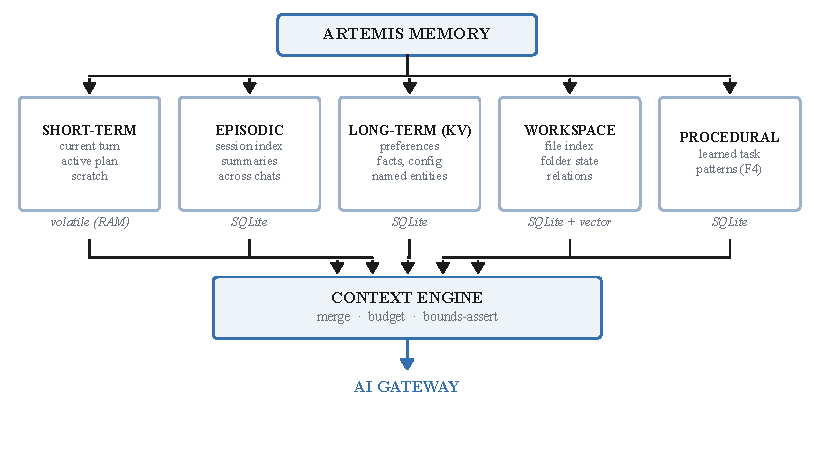
\includegraphics[width=\textwidth]{Figures/fig_memory.pdf}
    \caption{Five kinds of memory.}
    \label{fig:memory}
\end{figure}

\begin{figure}[tbp]
    \centering
    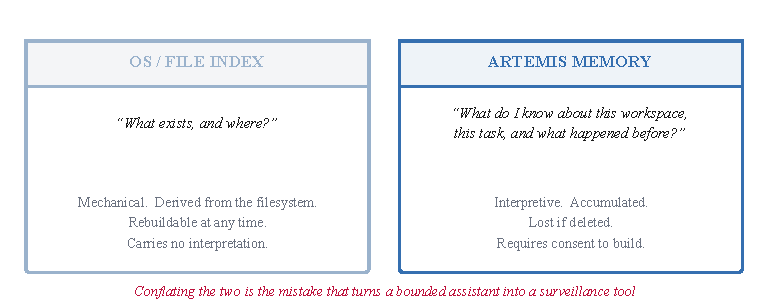
\includegraphics[width=\textwidth]{Figures/fig_memory_vs_index.pdf}
    \caption{The file index compared with system memory.}
    \label{fig:memoryindex}
\end{figure}

The two are answered to different questions and have different implications. The index is mechanical and rewritable; memory interpretive and, when erased, gone.

The file index provides an answer to what and where. It is mechanical, based on the filesystem and can be rebuilt at any time, and with no interpretation. Memory provides the answer of what the system has learned about a workspace, a task and the preferences of a user. It is interpretive, accumulated, lost when deleted and must be agreed upon to construct. The design makes them stay in different stores with different lifecycles, and each memory record is visible and removable individually in the disclosure panel. And it is in this way that the most demanded unmet capability, that the system should learn the organisational habits of the user, is accommodated, without any extension of the boundary: such learning is per-workspace memory, and is subject to the same visibility and deletion as any other.

\subsection{Disclosure as a Live Query}
The disclosure panel is not what the system writes about itself but a live query on all the stores. The rationale is that a written summary may be out-of-date or wrong, but a query may not be in disagreement with the data it reads. All rows can be deleted and deletion is a true cascade, such that deleting a workspace not only deletes its index directory, but also its file rows, its embeddings and its memory entries.

The alternative, of a periodically generated report, was rejected since it would render the trust claim persuasive as opposed to falsifiable and a falsifiable claim is the superior position. The audit log is not intended to be deleted, as it is based on the principle of an audit log whose subject matter can be deleted is not an audit log..

\subsection{The Remote Plane as a Detachable Component}
The remote access plane is drawn outside the core stack, and the test of whether that separation is genuine is that removing the entire plane leaves a fully functional single-machine system. Figure~\ref{fig:remote} shows its structure and Figure~\ref{fig:pairing} the pairing handshake.

\begin{figure}[tbp]
    \centering
    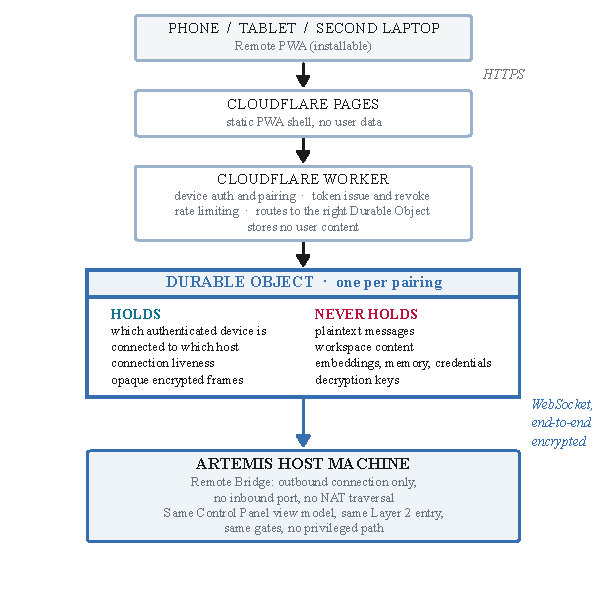
\includegraphics[width=0.92\textwidth]{Figures/fig_remote.pdf}
    \caption{The remote access plane.}
    \label{fig:remote}
\end{figure}

The durable object records which authenticated device is connected to which host and relays encrypted frames it cannot read.


Host-side confirmation is deliberate, so that possession of the pairing code alone is never sufficient to pair a device.

\begin{figure}[tbp]
    \centering
    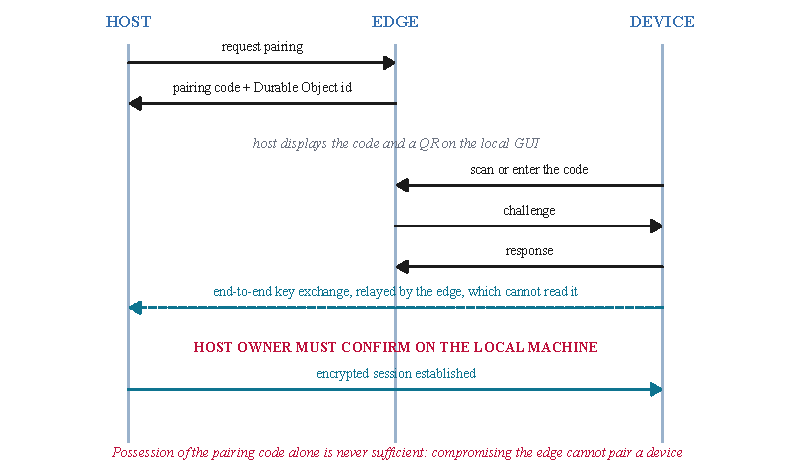
\includegraphics[width=\textwidth]{Figures/fig_pairing.pdf}
    \caption{The pairing handshake.}
    \label{fig:pairing}
\end{figure}

The plane is a control surface rather than a privilege escalation. Remote sessions run at equal or lower privilege than local ones and never higher. A workspace may be marked local-only, rendering it invisible to remote sessions. The outward actions can be set to need local approval irrespective of the location where the action is requested and this is the default. Sessions are time-based and on a host sleep, they are revoked by the host automatically and immediately, and all actions initiated by a remote user are recorded in the audit trail with their device. The relay does not possess plaintext of any type and thus the privacy assertion does not lose out on the edge compromise.

\subsection{Asynchrony with Bounded Queues}
Figure~\ref{fig:performance} illustrates that the interactive path is thin and all that is expensive is asynchronous. The indexing is done in a dynamic fashion, with only those chunks whose content hash is different re- embedded, thus a single line edit re-embeds only a single chunk instead of a file. The two-stage retrieval is two-pass retrieval, where the inexpensive vector recall is followed by a reranking pass that keeps the index small and yet does not compromise on quality. The local model is detained with idle timer such that the initial token is not charged a cold load.


The interactive path does not block when on background work and background progress is reported visibly and is cancellable.

\begin{figure}[tbp]
    \centering
    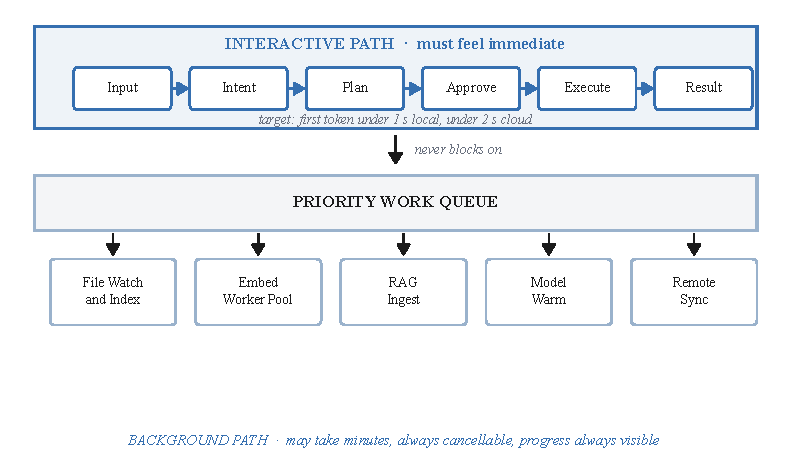
\includegraphics[width=\textwidth]{Figures/fig_performance.pdf}
    \caption{Asynchrony and background progress.}
    \label{fig:performance}
\end{figure}

Each queue is limited and a full queue releases the lowest-priority work and claims to have done so instead of expanding indefinitely. The rationale is that unbounded queues turn a load problem into a memory exhaustion problem and that a system that silently falls behind is one the behaviour of which the user cannot predict.t.

\section{Domain Model/Class Diagram}

The domain model will focus on four value objects that are immutable and five services that act on them. The value objects are not mutable in nature and hence a verdict cannot be attached to a call and the call manipulated before execution.

One of the proposed actions is called a ToolCall and contains an operation name, a workspace identifier, a list of paths relative to the workspace, arguments and a unique identifier. Its paths are relative, not absolute, such that an absolute path cannot be sneaked over the boundary by the loving care of its construction. It gives a description of previews and logs, and a fingerprint of the shape of the call regardless of what paths it crosses, which is the extent to which remembered approvals are used.

A Verdict is the end result of the policy engine, the decision on a single call, including the identification of the call it was applied to, the tier, the decision, the reason and the rule applied. It reveals the need of approval and whether the call was rejected, and can verify that it matches a particular call. It is that correspondence check, though, which prevents a call being a read and executed as a different kind of thing.

An ordered set of calls, having an intent, and an identifier is a Plan and the unit of approval and reversal.

A Resolved path is a path that has been asserted by all the assertions of the broker. This type is accepted by services and not a bare path so that an unchecked path does not accidentally access filesystem. To have one is the evidence that the line was crossed.

Services include the WorkspaceBroker, which addresses references or refuses; the PolicyEngine, which categorizes calls and remembers rules; the ApprovalBroker, which holds planned-to-be-done plans, constructs previews and records decisions; the UndoJournal, which records inverse operations and replays them; and the ToolDispatcher, which is the sole acting component.

This model has two relationships that bear the guarantees of the architecture. The dispatcher relies on the approval broker, instead of taking an approval flag provided by its caller, so that a service can not claim its authority. The dispatcher also solves paths via the broker in a second instance, although the policy engine has already done so, since the dispatcher is not allowed to rely on the previous component of the system having already executed its task correctly; that is what confused-deputy defects are about.

\begin{figure}[p]
\centering
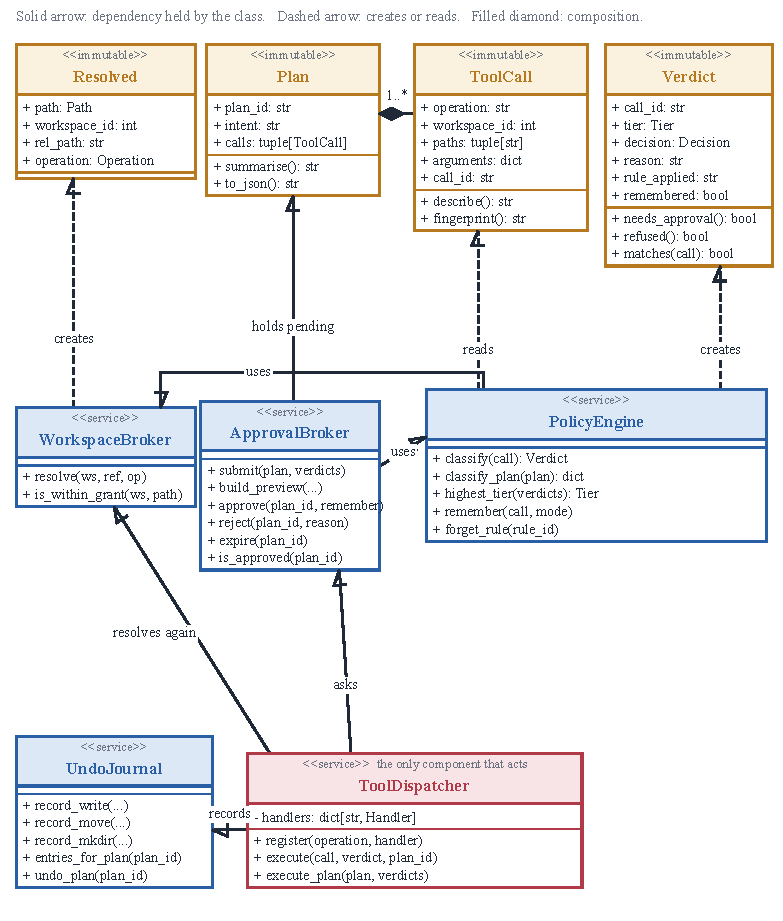
\includegraphics[width=\textwidth]{Figures/fig_class.pdf}
\caption{Class diagram.}
\label{fig:class}
\end{figure}

\section{Policies and Tactics}
This section specifies the policies and strategies that regulate implementation. They do not change the general structure, but outline the specifics of interface and implementation.

\subsection{Refusal as the Default Failure Mode}
All the vague states culminate in denial. An unknown operation is rejected but not as a read. A dead end is not attempted, but is rejected. A call with a verdict that is missing or mismatched is rejected. The execution can never be done by an expired approval and, that is why, the expiry is a unique result and not a type of rejection or silent rejection.

The other, explicit denial lists with permissive defaults, was discarded due to the fact that a denial list needs to know about all the dangerous operations whereas a permission list only needs to list the safe ones, and the result of an omission is of a different nature with the two.

\subsection{Single Enforcement Points}
Path resolution is carried out by the broker alone and execution by the dispatcher alone. Handler registration is an allowlist, which means that an operation that does not have a registered handler cannot be executed and the addition of a capability is an intentional action instead of an accidental result of a planner inventing a name.

One maintenance implication of this policy that must be declared to a future developer would be: adding a second path to the filesystem or a second point of execution would not be a refactoring but a change to what the system ensures, and would nullify the testing strategy, which relies on each. guarantee having one place at which it can be verified.

\subsection{Ordering Constraints}
There are three load-bearing orderings which cannot be changed. The containment test is preceded by canonisation. The mutation is preceded by the snapshot. Policy review is followed by dispatch. All these are properties of correctness, not matters of taste, and turning any of them about results in a system that seems to work but offers none of the assurance it asserts. They are then each covered by a special test the aim of which is to fail when the ordering is perturbed.

\subsection{Testing Strategy}
The structure of testing is structured around the guarantees and not the code structure. The boundary is probed adversarially, with the escape techniques including relative traversal, symbolic links to outside the grant, absolute paths, and sibling directories bearing a common prefix in name, which all have to be rejected and logged. Each of the sets of operations, and the unrecognised case are exhaustively tested on policy classification. The properties that nothing is approved by default and outward operations cannot be remembered are tested. Recovery is checked by performing a plan, undoing it and comparing the outcome with the state that was previously stored.

The build sequence ends at each stage with a gate test and the end of a stage is when the gate succeeds and not when the code exists. Gates are designed in such a way that they can fail, the most obvious example being the speech stage gate that fails in case voice demanded any new approval gate.

\subsection{Concurrency Handling}
The interactive route is single-threaded but the store is accessed by over one thread, as the file watcher flushes its debounce buffer on a clock. The store thus serialises all its statements behind a lock, and all access is via its guarded means, as opposed to access to the connection itself. Disabling the thread guard on the database engine itself without this lock would trade a noticeable crash with an imperceptible corruption, thus the pair cannot be separated.

Chain read and append operations on the audit log are performed under one lock, and thus, two threads cannot chain on the same predecessor and bifurcate the chain.

\subsection{Source Organisation}
The source is structured according to architectural role and not by feature in order to have the correspondence between the design and the code direct. The fundamental elements, i.e., the broker, the policy engine, the approval broker, the undo journal, the dispatcher and the disclosure panel, are contained in a single package. Another plane is the data plane. The surfaces of interfaces are in a third place. A reader in need of the enforcement point of a guarantee can find it where the architecture claims it is.


\section{Conclusion}
This chapter has introduced the system design: the layers and their components, the strategies that shape the architecture, domain model and the policies that bind the design. Each significant decision was traced to a requirement or a research finding. The design puts the path resolution, classification and execution in one component, and the remote plane is detachable so that the guarantees which the hypothesis relies on are structural properties and can be tested as such. The following chapter details the prototype which realizes this design and tests which are exercising the design..

\chapter{Implementation and Test Cases}
This chapter explains the prototype that was constructed throughout the initial phase of the project and the tests that exercise this prototype. Since the first deliverable is possible in the template, the implementation section will be a description of the prototype and not of a complete product. It gives the platform and interfaces used, the algorithms behind the components that are not apparent from the design, and the state of each stage of the build sequence. In the second part the design of the test cases is established and a representative set is given in the specified layout, each follow-up to the requirements of Chapter 4. The third section presents the test measurements and requirements traceability to tests. The chapter does not copy the source code, but documents the processes that the code executes..

\section{Implementation}
\subsection{Scope and Status of the Prototype}
The prototype is a working desktop assistant written in Python 3.13. It comprises 56 modules and about 14,250 lines of source, organised by architectural role into five packages as Chapter 6 describes: the core enforcement layer (26 modules, about 5,400 lines), the local data plane (4 modules, about 850 lines), the capability services (10 modules, about 2,100 lines), the presentation surfaces (5 modules, about 4,450 lines) and the optional remote plane (10 modules, about 1,450 lines). A further relay program in JavaScript and a phone page complete the remote plane. It is accompanied by an automated suite of 554 tests.

All eight stages of the build sequence of Table~\ref{tab:build} have been implemented, each ending in the gate test that Chapter 5 requires. Table~\ref{tab:status} records the state of each stage. A stage counts as having its gate passing when the automated suite passes. It counts as validated through the interface only where the user-interface campaign of Chapter 9 supports it, and that campaign found a number of defects that the automated gates did not, so the two columns are reported separately.

{\Needspace*{7\baselineskip}
\begin{longtable}{|p{0.9cm}|p{4.6cm}|p{3.4cm}|p{4.5cm}|}
\caption{Implementation status by stage.}\label{tab:status}\\*
\hline
\textbf{Stage} & \textbf{Deliverable} & \textbf{Automated gate} & \textbf{Interface campaign (Chapter 9)} \\*
\hline
\endfirsthead
\caption[]{continued from previous page}\\*
\hline
\textbf{Stage} & \textbf{Deliverable} & \textbf{Automated gate} & \textbf{Interface campaign (Chapter 9)} \\*
\hline
\endhead
\hline
1 & Workspace foundation & Passing & Gate partly met; folder guard-rails missing \\*
\hline
2 & Policy, approval and undo & Passing & Gate partly met; undo defect on name collisions \\*
\hline
3 & Gateway: router, context, planner, dispatcher & Passing & Gate met for execution; one retrieval isolation failure \\
\hline
4 & Resume, tidy, repeated tasks & Passing & Gate partly met \\
\hline
5 & Notes synthesis and code assistance & Passing & Gate not met: unsupported claims not always labelled \\
\hline
6 & Web search, mail, drafting & Passing & Gate met; visibility of what left the computer weak \\
\hline
7 & Speech input and output & Passing & Gate met (no new approval gate); recording control defect \\
\hline
8 & Remote access plane & Passing & Not fully tested; one boundary defect \\
\hline
\end{longtable}
}

\subsection{Platform and Interfaces}
Table~\ref{tab:platform} lists the platform, libraries and services on which the prototype depends and the role of each. Every dependency of the core is local. The network is used only by the optional cloud providers, the web search service, the mail account and the remote plane, each behind its own gate.

{\Needspace*{7\baselineskip}
\begin{longtable}{|p{4.2cm}|p{9.2cm}|}
\caption{Platform, libraries and services.}\label{tab:platform}\\*
\hline
\textbf{Component} & \textbf{Role} \\*
\hline
\endfirsthead
\caption[]{continued from previous page}\\*
\hline
\textbf{Component} & \textbf{Role} \\*
\hline
\endhead
\hline
Python 3.13, pytest & Implementation language and test runner (554 tests). \\*
\hline
SQLite~\cite{ref:sqlite} & The system of record: workspaces, file index, audit log, undo journal, chat sessions, settings; one vector index database per workspace. \\*
\hline
Ollama~\cite{ref:ollama}, model gemma4:e4b & Default local language model, reached over the loopback interface; model name is a user setting. \\
\hline
nomic-embed-text through Ollama & Local text embedder for the vector index. \\
\hline
Cloud providers (Gemini, OpenAI, Anthropic) & Optional fallback tiers, available only to workspaces that opted in. \\
\hline
LangGraph~\cite{ref:langgraph} & State-graph runtime for the planner, with an explicit pause before any gated call. \\
\hline
NumPy & Cosine similarity over a workspace's embedding matrix. \\
\hline
watchdog & File watcher feeding incremental indexing. \\
\hline
Gradio 6.12 & The web interface with tabs Work, Folders, What it knows and Settings. \\
\hline
PySide6, Typer & A desktop panel and a command-line surface over the same components. \\
\hline
faster-whisper & Local speech recognition. \\
\hline
Kokoro, Piper, Windows speech & Speech synthesis, tried in that order. \\
\hline
cryptography, keyring & X25519, HKDF and AES-256-GCM for the remote plane; storage of keys and passwords in the operating system keyring. \\
\hline
Cloudflare Worker with a Durable Object & The deployed relay of the remote plane and the host of the phone page. \\
\hline
\end{longtable}
}

\subsection{Implementation of the Workspace Broker}
A path is only created when the only component that transforms a reference into a path is the broker. It implements five claims in a given order: the reference is resolved against the root grant; it is canonicalised, the symbolic links and parent-directory elements are substituted by the actual location; the canonical path is checked to be contained within the grant root; it is checked against a denylist; and the requested operation is checked against the permission of the grant. The canonicalisation comes before the containment test in that a symbolic link in the grant which has its target out of the grant appears contained until it is resolved. Credential and system files and locations, including .ssh, .aws, .env and key files, are always included in the denylist, and the store of the application itself is always included, so that a grant on a parent folder does not reveal the audit log. An effective solution provides a value that documents the workstation, the relative path and the operation. Only this value can be used by services and not a bare path, so an uncontrolled path cannot accidentally reach the file system. Each refusal is documented to the audit log prior to the refusal being raised.

\subsection{Implementation of the Policy Engine and Approval Broker}
A proposed call is all the policy engine reads. It does not even look at the text of the model, so whatever is written in the inner part of any document cannot be able to defend itself to a new decision. The evaluation is executed in a fixed order, i.e. the grant check, the destructive check, the egress check, the mutation check and lastly allow, the first rule that matches is the deciding one. The call is made in only one tier. No approval of reads. Changes made are reversible except when the user has selected to permit that operation without question in that workspace. Actions towards the outside are never kept and cannot ever be recalled. Unrecognised destructive operations are denied a permission course and an unrecognised operation is denied also, such that nothing omitted can ever broaden the permission. The top level of the steps of a plan is the top level. Classification never makes any mistake: a call that is not classifiable is a refusal.

The approval broker keeps each plan in one of four states, being pending, approved, rejected and expired, and none of the transitions out of pending is automatic. One plan may not be voted twice, expiry is not a form of approval and an approved plan is scoped to a single operation within a single workspace. The preview displays the workspace, the suggested operations, the level, whether something leaves the computer and whether something is deleted and in outward steps displays the specific search text or message body which the user approves of what actually will be done.

\subsection{Implementation of the Dispatcher and the Undo Journal}
The only component that operates is the dispatcher. It refuses each call in order: a call having no verdict is refused; a verdict delivered in respect of a different call is refused, since each verdict is marked by the identifier of the call; a denied call is never executed; a gated call is refused unless the approval broker has a recorded approval to its plan. The caller never passes the approval but looks up the approval. The dispatcher also finds the paths of the call by the execution time via the broker, hence, the boundary is even when a previous layer was skipped.

The undo journal documents the method of undoing a change prior to the change. A copy of a small file is moved into a content-addressed blob store: thus, the same data is stored only once, and a file larger than four mebibytes is hard-linked where the file system allows. A motion or a newly generated file does not require a copy since it is inverse structural. Undo operates at a plan-granularity, undoing all the recorded steps in reverse order, and leaving a folder, filled in by the user in the meantime. Both the dispatcher and the journal write to an append-only audit log where each entry has the hash of the last entry such that deleting or modifying an entry will cause the chain to break, and on-demand the chain can be checked. Chain read and append are actions performed under a single lock thereby preventing forking of the chain by two threads.

\subsection{Implementation of the Gateway}
The typed request is first sent through an intent step which determines whether the request is a question, a file task, a draft, a search, a mail request or a request about code. It is rule-based, with patterns applied to the request text so routing is deterministic, quick and verifiable and does not rely upon the opinion of a model. The model router then chooses a provider. Providers are retried in tiers order, starting with local ones, and with a single retry per tier, so that a dead chain will fall over in seconds and with a failure notice. Egress is also determined by the router which is the only location to determine a workspace that has not subscribed to cloud has an exclusive tier to the workspace and when local model is inaccessible the response is denial and not silent upgrading to a cloud provider.

The context engine puts together what the model can see. Every fragment has its provenance, is the text of the user, a workspace file, a tool output, memory or the web. The words of the user are the only authority, all other sources are displayed to the model as data. The active workspace limit retrieval and the context size is budgeted with an estimate of 3.6 characters per token. The planner is a LangGraph state graph, which requests the model to give a structured plan of a low sampling temperature of 0.1, verifies it against the plannable operations and gives up to three planning cycles with a time budget of 30 seconds, and plans, but does not execute. The model can thus suggest, but has no handle by which it can act.

\subsection{Implementation of Indexing, Retrieval and Grounding}
The files within a workspace are partitioned into slices of not more than 800 characters with its source file and line range so a citation can be made referring to it. The local embedder normalizes each chunk, and stores it as a float32 vector in a workspace-private database. A search inserts the query, and calculates the cosine similarity with the matrix in the workspace in a single product of matrices, returning the optimal chunks. The indexing is incremental: a file that has not changed in content is not re-embedded, files larger than two mebibytes are not indexed, and an indexing worker does not block the interactive path. Changes are signalled to the index using a file watcher that has a debounce buffer.

A grounding gate is put on each response to a question regarding the files of the user. The answer is divided into claims, each in a sentence and a claim is justified when it has a citation that identifies a chunk sent to the model and is a file chunk and not the words of the user. Any other claim is indicated with an unsubstantiated label. The gate provides that there is a source and that a source has been given and does not provide that the source states what the claim states that it is a restriction which is inherited by the literature and recorded as such in Chapter 3.

\subsection{Implementation of the Capability Services}
Only the dispatcher and the broker can access the file system through all services. When you resume, the files that were last in a workspace are restored along with a note that was left by the user to resume. Arrange loose files in a folder by type, with extension tables of documents, spreadsheets, pictures and others, or by date as required. Before making the moves, it preplans the creation of each destination folder and leaves behind a file that has no counterpart of its type and files that have already been filed in subfolders, assigns a conflicting name a different name rather than an overwrite, and displays every move in the preview. The service has no deletion operation to make a call. Repeated- task detection calculates a signature on each approved plan, and ignores undone plans and plans the user has rejected, and provides an automation when the signature has been repeated at least three times over a 30-day window. Code assistance finds responses to code questions and presents any proposed change as a difference, and nothing in the service writes to a file. Web search only operates on an explicit query, via a public search endpoint, displaying the query in the preview, logs all queries, and labels results as web searches. Mail only sends a draft using the mail account of the user, after the draft is approved; the recipient is authenticated, header injection is not allowed and the recipient and time of each send are logged. Drafting creates a new file whose name will not conflict with any existing file and will never replace it; undo deletes it.

\subsection{Implementation of Disclosure}
The panel with the title What ARTEMIS knows is a live query of the store and is not a cached list. It lists every workspace, every indexed file, the hidden chunks, remembered facts, retained chats, automation rules, policy exceptions and the history of outward actions, and it also has a deletion of each item, with a confirmation, other than the audit log. Deleting a workspace removes the index entries, embeddings, sessions, memory and rules based on it and leaves files owned by the user unaffected.

\subsection{Implementation of Speech}
Speech is an interaction layer modality but not a service. Audio will also be accepted as long as a voice session is armed by the user. Faster-whisper transcribes a recording on the computer, which is deleted once read and even when transcribing fails. The audit trail documents that it was voice and not what was said. The transcript is sent to precisely the same point of entry as the typed request thus a spoken request is subjected to the same gates and a spoken email is awaited approval like a typed one. Replies will be read out by the first of three engines which will be tried in the order of naturalness. In front of speech, the reply is deprived of the model label and of markup and is trimmed, and a spoken chat is phrased as speech. The hands-free loop is contained in the browser: once it has listened to a reply, it considers a silence of approximately 3.5 seconds after the user has spoken as the end of the user turn, and, when the user takes over four seconds to say anything, it speaks first and then resumes listening.

\subsection{Implementation of the Remote Plane}
The distant airplane allows a matched phone to communicate with the computer using a relay that transports opaque frames with no other knowledge. An exchange of X25519 keys where the short pairing code is concatenated into the derived key are done to pair the devices such that a relay that replaces keys learns nothing, and the owner of the device confirms on the computer after comparing a short safety number. AES-256-GCM is used to seal frames with a per-session key and counters, such that a replayed frame will not be answered twice. The key of the phone is stored as a non-extractable key in the browser and the key of the host in keyring of the operating system. One hour is one session which then has to be opened again. The bridge reveals asking and answering only: folders are not visible on a device unless they are ticked, no outward approvals can be received on a device, it must provide on the computer, voice on a device is default, and each remote request is logged against its device. Revocation of a device is immediate. In voice, the phone transmits small blocks of 16 kHz audio over the encrypted channel, the computer determines when the turn is over by counting audio time and the response is sent back sentence by sentence as text and speech. The plane is optional in nature, in that nothing in the core brings in the remote package, and the main database contains no remote tables. The relay is implemented as a Cloudflare Worker with a Durable Object serving the phone page, and a runnable relay with the same rules is made available to use on a home network and to test.

\subsection{Implementation of the User Interface}
There are four areas in the web interface. The request box, the folder selector, the approval cards and the saved chats, which storage lasts seven days, are stored in work, along with the voice controls. Workspaces are added and listed by typed path by Folders. The disclosure panel is what it knows. The settings contain the model options, the cloud policy per folder, the mail account and the remote access controls. Gradio 6.12 limits interaction somewhat, and the interface operates within those limits by utilizing hidden controls which are invoked by scripts in the page. The identical elements can be accessed by a command line and a desktop panel.

\section{Test case Design and description}
The tests get structured on the guarantees of Chapter 4 and not on the code structure. The following are their common attributes. Each test is run against a throwaway store, which has been chosen by an environment variable, and against a throwaway folder which represents the files of the user, such that none of the tests touch real data, and tests do not interfere with one another. No test requires the network, a cloud key or a running language model: model responses are provided by stub providers, embeddings by a deterministic fake embedder, mail and search by stubs, and speech recognition and synthesis by stand-ins. The suite thus verifies the enforcement layer and the plumbing deterministically and is unable to verify the quality of what a real model claims. Tested Gate tests are written in such a way that they fail, in order to test a property an attempt at breaking the gate: escaping the boundary, an unknown operation to the policy engine, a call with an unknown verdict to the dispatcher, and a requirement of any new approval path in the case of speech. Every test case below indicates the tests it summarises and the tables are in the format required by the template..

\subsection{Test Cases}
The nine test cases below are TC-01 to TC-09, in Tables~\ref{tab:tc1} to \ref{tab:tc9}.

{\small
\Needspace*{7\baselineskip}
\begin{longtable}{|p{2.4cm}p{5.0cm}p{2.4cm}p{3.8cm}|}
\caption{Test case TC-01: workspace boundary.}\label{tab:tc1}\\*
\endfirsthead
\caption[]{continued from previous page}\\*
\endhead
\hline
\multicolumn{4}{|c|}{\textbf{Workspace Broker}} \\* \hline
\multicolumn{4}{|p{14.8cm}|}{\textbf{Requirements FR-2, FR-3, FR-4; stage gate of the workspace foundation stage (tests/test\_broker.py, 13 tests)}} \\* \hline
\multicolumn{2}{|p{7.8cm}|}{\textbf{Test Case ID:} TC-01} &
  \multicolumn{2}{p{6.6cm}|}{\textbf{QA Test Engineer:} Project team (automated suite)} \\* \hline
\multicolumn{2}{|p{7.8cm}|}{\textbf{Test case Version:} 1.0} &
  \multicolumn{2}{p{6.6cm}|}{\textbf{Reviewed By:} Project team} \\* \hline
\multicolumn{2}{|p{7.8cm}|}{\textbf{Test Date:} 9 November 2026} &
  \multicolumn{2}{p{6.6cm}|}{\textbf{Use Case Reference(s):} UC-1, UC-3} \\ \hline
\multicolumn{1}{|p{2.4cm}|}{\textbf{Revision History:}} &
  \multicolumn{3}{p{12.0cm}|}{None; first version.} \\ \hline
\multicolumn{1}{|p{2.4cm}|}{\textbf{Objective:}} &
  \multicolumn{3}{p{12.0cm}|}{Establish that no reference can resolve to a path outside an active grant, that every attempt is recorded, and that the record is intact.} \\ \hline
\multicolumn{1}{|p{2.4cm}|}{\textbf{Product/Ver/ Module:}} &
  \multicolumn{3}{p{12.0cm}|}{A.R.T.E.M.I.S. prototype, core layer. The broker is the single component that turns a reference into a path.} \\ \hline
\multicolumn{1}{|p{2.4cm}|}{\textbf{Environment:}} &
  \multicolumn{3}{p{12.0cm}|}{Windows 10 Pro, Python 3.13, pytest. Each test runs against a throwaway store (ARTEMIS\_HOME set to a temporary folder) and a throwaway folder standing in for the user's files. No network, no cloud key and no language model are needed.} \\ \hline
\multicolumn{1}{|p{2.4cm}|}{\textbf{Assumptions:}} &
  \multicolumn{3}{p{12.0cm}|}{The machine can create symbolic links (checked at run time; the symbolic link case is skipped otherwise).} \\ \hline
\multicolumn{1}{|p{2.4cm}|}{\textbf{Pre-Requisite:}} &
  \multicolumn{3}{p{12.0cm}|}{A folder with two files is granted as a workspace; a second folder holding a file named secrets.txt exists beside it and is not granted.} \\ \hline
\multicolumn{1}{|p{2.4cm}|}{\textbf{Step No.}} &
  \multicolumn{1}{p{5.0cm}|}{\textbf{Execution description}} &
  \multicolumn{2}{p{6.6cm}|}{\textbf{Procedure result}} \\ \hline
\multicolumn{1}{|p{2.4cm}|}{1} & \multicolumn{1}{p{5.0cm}|}{Resolve readme.txt inside the grant.} & \multicolumn{2}{p{6.6cm}|}{A resolved path is returned, with the workspace identifier and the relative path.} \\ \hline
\multicolumn{1}{|p{2.4cm}|}{2} & \multicolumn{1}{p{5.0cm}|}{Resolve references that climb out of the grant with parent-directory segments.} & \multicolumn{2}{p{6.6cm}|}{A boundary refusal is raised with the reason outside grant.} \\ \hline
\multicolumn{1}{|p{2.4cm}|}{3} & \multicolumn{1}{p{5.0cm}|}{Place a symbolic link inside the grant that points at the ungranted folder, then resolve a file through it.} & \multicolumn{2}{p{6.6cm}|}{Refused. The link looks contained; only its canonical target is not, which is what canonicalising first exists to catch.} \\ \hline
\multicolumn{1}{|p{2.4cm}|}{4} & \multicolumn{1}{p{5.0cm}|}{Resolve an absolute path and a sibling folder whose name begins with the grant's name.} & \multicolumn{2}{p{6.6cm}|}{Both refused; a shared name prefix is not containment.} \\ \hline
\multicolumn{1}{|p{2.4cm}|}{5} & \multicolumn{1}{p{5.0cm}|}{Read the audit log after a refused attempt.} & \multicolumn{2}{p{6.6cm}|}{One refused entry exists for the attempt and contains the reference text; the hash chain verifies.} \\ \hline
\multicolumn{4}{|p{14.8cm}|}{\textbf{Comments:} All 13 tests passed, including the symbolic link case on the test machine.} \\ \hline
\multicolumn{4}{|c|}{\textbf{Passed [X]\quad Failed [\ ]\quad Not Executed [\ ]}} \\ \hline
\end{longtable}
}

{\small
\Needspace*{7\baselineskip}
\begin{longtable}{|p{2.4cm}p{5.0cm}p{2.4cm}p{3.8cm}|}
\caption{Test case TC-02: policy engine classification.}\label{tab:tc2}\\*
\endfirsthead
\caption[]{continued from previous page}\\*
\endhead
\hline
\multicolumn{4}{|c|}{\textbf{Policy Engine}} \\* \hline
\multicolumn{4}{|p{14.8cm}|}{\textbf{Requirements FR-7, FR-8, FR-9, FR-10, FR-11 (tests/test\_policy.py, 17 tests)}} \\* \hline
\multicolumn{2}{|p{7.8cm}|}{\textbf{Test Case ID:} TC-02} &
  \multicolumn{2}{p{6.6cm}|}{\textbf{QA Test Engineer:} Project team (automated suite)} \\* \hline
\multicolumn{2}{|p{7.8cm}|}{\textbf{Test case Version:} 1.0} &
  \multicolumn{2}{p{6.6cm}|}{\textbf{Reviewed By:} Project team} \\* \hline
\multicolumn{2}{|p{7.8cm}|}{\textbf{Test Date:} 9 November 2026} &
  \multicolumn{2}{p{6.6cm}|}{\textbf{Use Case Reference(s):} UC-2, UC-3} \\ \hline
\multicolumn{1}{|p{2.4cm}|}{\textbf{Revision History:}} &
  \multicolumn{3}{p{12.0cm}|}{None; first version.} \\ \hline
\multicolumn{1}{|p{2.4cm}|}{\textbf{Objective:}} &
  \multicolumn{3}{p{12.0cm}|}{Show that the four tiers behave as specified and that the destructive tier has no approval path.} \\ \hline
\multicolumn{1}{|p{2.4cm}|}{\textbf{Product/Ver/ Module:}} &
  \multicolumn{3}{p{12.0cm}|}{A.R.T.E.M.I.S. prototype, core layer. Classification reads the tool call only and never the model's reasoning.} \\ \hline
\multicolumn{1}{|p{2.4cm}|}{\textbf{Environment:}} &
  \multicolumn{3}{p{12.0cm}|}{Windows 10 Pro, Python 3.13, pytest. Each test runs against a throwaway store (ARTEMIS\_HOME set to a temporary folder) and a throwaway folder standing in for the user's files. No network, no cloud key and no language model are needed.} \\ \hline
\multicolumn{1}{|p{2.4cm}|}{\textbf{Assumptions:}} &
  \multicolumn{3}{p{12.0cm}|}{Remembered approvals are off by default.} \\ \hline
\multicolumn{1}{|p{2.4cm}|}{\textbf{Pre-Requisite:}} &
  \multicolumn{3}{p{12.0cm}|}{A folder is granted as a workspace.} \\ \hline
\multicolumn{1}{|p{2.4cm}|}{\textbf{Step No.}} &
  \multicolumn{1}{p{5.0cm}|}{\textbf{Execution description}} &
  \multicolumn{2}{p{6.6cm}|}{\textbf{Procedure result}} \\ \hline
\multicolumn{1}{|p{2.4cm}|}{1} & \multicolumn{1}{p{5.0cm}|}{Classify a read of a file inside the workspace.} & \multicolumn{2}{p{6.6cm}|}{Allowed to run without asking.} \\ \hline
\multicolumn{1}{|p{2.4cm}|}{2} & \multicolumn{1}{p{5.0cm}|}{Classify a change to a file and a call that sends something out of the computer.} & \multicolumn{2}{p{6.6cm}|}{Both held for approval; the second is flagged as leaving the computer.} \\ \hline
\multicolumn{1}{|p{2.4cm}|}{3} & \multicolumn{1}{p{5.0cm}|}{Classify a delete operation.} & \multicolumn{2}{p{6.6cm}|}{Tier destructive, decision refuse. No approval can change this.} \\ \hline
\multicolumn{1}{|p{2.4cm}|}{4} & \multicolumn{1}{p{5.0cm}|}{Classify an operation the engine has never heard of (rm\_rf).} & \multicolumn{2}{p{6.6cm}|}{Refused under the rule unknown-operation, not assumed safe.} \\ \hline
\multicolumn{1}{|p{2.4cm}|}{5} & \multicolumn{1}{p{5.0cm}|}{Classify a read whose path escapes the grant.} & \multicolumn{2}{p{6.6cm}|}{Refused under grant-check, which runs before every other rule.} \\ \hline
\multicolumn{1}{|p{2.4cm}|}{6} & \multicolumn{1}{p{5.0cm}|}{Ask to remember an outward action and a destructive action.} & \multicolumn{2}{p{6.6cm}|}{Both remain gated or refused; remembering is scoped to one operation in one workspace.} \\ \hline
\multicolumn{4}{|p{14.8cm}|}{\textbf{Comments:} All 17 tests passed.} \\ \hline
\multicolumn{4}{|c|}{\textbf{Passed [X]\quad Failed [\ ]\quad Not Executed [\ ]}} \\ \hline
\end{longtable}
}

{\small
\Needspace*{7\baselineskip}
\begin{longtable}{|p{2.4cm}p{5.0cm}p{2.4cm}p{3.8cm}|}
\caption{Test case TC-03: tool dispatcher.}\label{tab:tc3}\\*
\endfirsthead
\caption[]{continued from previous page}\\*
\endhead
\hline
\multicolumn{4}{|c|}{\textbf{Tool Dispatcher}} \\* \hline
\multicolumn{4}{|p{14.8cm}|}{\textbf{Requirements FR-17, FR-35; invariants of Chapter 6 (tests/test\_dispatch.py, 11 tests)}} \\* \hline
\multicolumn{2}{|p{7.8cm}|}{\textbf{Test Case ID:} TC-03} &
  \multicolumn{2}{p{6.6cm}|}{\textbf{QA Test Engineer:} Project team (automated suite)} \\* \hline
\multicolumn{2}{|p{7.8cm}|}{\textbf{Test case Version:} 1.0} &
  \multicolumn{2}{p{6.6cm}|}{\textbf{Reviewed By:} Project team} \\* \hline
\multicolumn{2}{|p{7.8cm}|}{\textbf{Test Date:} 9 November 2026} &
  \multicolumn{2}{p{6.6cm}|}{\textbf{Use Case Reference(s):} UC-2} \\ \hline
\multicolumn{1}{|p{2.4cm}|}{\textbf{Revision History:}} &
  \multicolumn{3}{p{12.0cm}|}{None; first version.} \\ \hline
\multicolumn{1}{|p{2.4cm}|}{\textbf{Objective:}} &
  \multicolumn{3}{p{12.0cm}|}{Show that the dispatcher cannot be talked into acting without a verdict and an approval, and that a full plan can be gated, executed and undone.} \\ \hline
\multicolumn{1}{|p{2.4cm}|}{\textbf{Product/Ver/ Module:}} &
  \multicolumn{3}{p{12.0cm}|}{A.R.T.E.M.I.S. prototype, core layer. The dispatcher is the only component that acts.} \\ \hline
\multicolumn{1}{|p{2.4cm}|}{\textbf{Environment:}} &
  \multicolumn{3}{p{12.0cm}|}{Windows 10 Pro, Python 3.13, pytest. Each test runs against a throwaway store (ARTEMIS\_HOME set to a temporary folder) and a throwaway folder standing in for the user's files. No network, no cloud key and no language model are needed.} \\ \hline
\multicolumn{1}{|p{2.4cm}|}{\textbf{Assumptions:}} &
  \multicolumn{3}{p{12.0cm}|}{Handlers are registered by the services; unregistered operations have none.} \\ \hline
\multicolumn{1}{|p{2.4cm}|}{\textbf{Pre-Requisite:}} &
  \multicolumn{3}{p{12.0cm}|}{A granted workspace with a file readme.txt containing the word hello.} \\ \hline
\multicolumn{1}{|p{2.4cm}|}{\textbf{Step No.}} &
  \multicolumn{1}{p{5.0cm}|}{\textbf{Execution description}} &
  \multicolumn{2}{p{6.6cm}|}{\textbf{Procedure result}} \\ \hline
\multicolumn{1}{|p{2.4cm}|}{1} & \multicolumn{1}{p{5.0cm}|}{Execute a read call with no verdict.} & \multicolumn{2}{p{6.6cm}|}{Refused: no policy verdict.} \\ \hline
\multicolumn{1}{|p{2.4cm}|}{2} & \multicolumn{1}{p{5.0cm}|}{Execute a change to readme.txt after classification but without an approval for its plan.} & \multicolumn{2}{p{6.6cm}|}{Refused: needs approval. The file still contains hello.} \\ \hline
\multicolumn{1}{|p{2.4cm}|}{3} & \multicolumn{1}{p{5.0cm}|}{Execute a call the policy denied, and a call for an operation with no handler.} & \multicolumn{2}{p{6.6cm}|}{Neither executes.} \\ \hline
\multicolumn{1}{|p{2.4cm}|}{4} & \multicolumn{1}{p{5.0cm}|}{Execute a call whose path escapes the workspace, with a verdict that claims otherwise.} & \multicolumn{2}{p{6.6cm}|}{Refused again at execution, so the boundary holds even if an earlier layer is bypassed.} \\ \hline
\multicolumn{1}{|p{2.4cm}|}{5} & \multicolumn{1}{p{5.0cm}|}{Run a full plan: classify, submit, approve, execute, undo.} & \multicolumn{2}{p{6.6cm}|}{Gated, executed once, snapshotted before the change, and restored by undo; every refusal reaches the audit log.} \\ \hline
\multicolumn{4}{|p{14.8cm}|}{\textbf{Comments:} All 11 tests passed.} \\ \hline
\multicolumn{4}{|c|}{\textbf{Passed [X]\quad Failed [\ ]\quad Not Executed [\ ]}} \\ \hline
\end{longtable}
}

{\small
\Needspace*{7\baselineskip}
\begin{longtable}{|p{2.4cm}p{5.0cm}p{2.4cm}p{3.8cm}|}
\caption{Test case TC-04: undo of an approved plan.}\label{tab:tc4}\\*
\endfirsthead
\caption[]{continued from previous page}\\*
\endhead
\hline
\multicolumn{4}{|c|}{\textbf{Undo Journal}} \\* \hline
\multicolumn{4}{|p{14.8cm}|}{\textbf{Requirements FR-15, FR-16 (tests/test\_undo.py, 10 tests)}} \\* \hline
\multicolumn{2}{|p{7.8cm}|}{\textbf{Test Case ID:} TC-04} &
  \multicolumn{2}{p{6.6cm}|}{\textbf{QA Test Engineer:} Project team (automated suite)} \\* \hline
\multicolumn{2}{|p{7.8cm}|}{\textbf{Test case Version:} 1.0} &
  \multicolumn{2}{p{6.6cm}|}{\textbf{Reviewed By:} Project team} \\* \hline
\multicolumn{2}{|p{7.8cm}|}{\textbf{Test Date:} 9 November 2026} &
  \multicolumn{2}{p{6.6cm}|}{\textbf{Use Case Reference(s):} UC-2} \\ \hline
\multicolumn{1}{|p{2.4cm}|}{\textbf{Revision History:}} &
  \multicolumn{3}{p{12.0cm}|}{None; first version.} \\ \hline
\multicolumn{1}{|p{2.4cm}|}{\textbf{Objective:}} &
  \multicolumn{3}{p{12.0cm}|}{Show that recovery information is recorded before a change and that undo restores the state the user approved from.} \\ \hline
\multicolumn{1}{|p{2.4cm}|}{\textbf{Product/Ver/ Module:}} &
  \multicolumn{3}{p{12.0cm}|}{A.R.T.E.M.I.S. prototype, core layer. Snapshots are kept in a local blob store; moves need no copy.} \\ \hline
\multicolumn{1}{|p{2.4cm}|}{\textbf{Environment:}} &
  \multicolumn{3}{p{12.0cm}|}{Windows 10 Pro, Python 3.13, pytest. Each test runs against a throwaway store (ARTEMIS\_HOME set to a temporary folder) and a throwaway folder standing in for the user's files. No network, no cloud key and no language model are needed.} \\ \hline
\multicolumn{1}{|p{2.4cm}|}{\textbf{Assumptions:}} &
  \multicolumn{3}{p{12.0cm}|}{Files are below the hardlink threshold unless stated.} \\ \hline
\multicolumn{1}{|p{2.4cm}|}{\textbf{Pre-Requisite:}} &
  \multicolumn{3}{p{12.0cm}|}{A granted workspace with two files, readme.txt and notes/chapter3.md.} \\ \hline
\multicolumn{1}{|p{2.4cm}|}{\textbf{Step No.}} &
  \multicolumn{1}{p{5.0cm}|}{\textbf{Execution description}} &
  \multicolumn{2}{p{6.6cm}|}{\textbf{Procedure result}} \\ \hline
\multicolumn{1}{|p{2.4cm}|}{1} & \multicolumn{1}{p{5.0cm}|}{Record the creation of a Drafts folder and the moves of both files into it, performing each change after its record is written.} & \multicolumn{2}{p{6.6cm}|}{Both files sit in Drafts; the originals are gone.} \\ \hline
\multicolumn{1}{|p{2.4cm}|}{2} & \multicolumn{1}{p{5.0cm}|}{Undo the plan by its identifier.} & \multicolumn{2}{p{6.6cm}|}{Three steps reversed, no problems reported.} \\ \hline
\multicolumn{1}{|p{2.4cm}|}{3} & \multicolumn{1}{p{5.0cm}|}{Inspect the workspace.} & \multicolumn{2}{p{6.6cm}|}{Both files are back at their original paths and the created folder is removed.} \\ \hline
\multicolumn{1}{|p{2.4cm}|}{4} & \multicolumn{1}{p{5.0cm}|}{Undo a plan after the user has put a new file into the created folder.} & \multicolumn{2}{p{6.6cm}|}{The folder is kept, because removing it would destroy the user's file.} \\ \hline
\multicolumn{1}{|p{2.4cm}|}{5} & \multicolumn{1}{p{5.0cm}|}{Undo an unknown plan, and undo the same plan twice.} & \multicolumn{2}{p{6.6cm}|}{Reported, not raised; a reversed plan is cleared from the journal; each undo is written to the audit log.} \\ \hline
\multicolumn{4}{|p{14.8cm}|}{\textbf{Comments:} All 10 tests passed. The campaign of Section~\ref{sec:campaign} later found a name-collision case that these tests do not cover.} \\ \hline
\multicolumn{4}{|c|}{\textbf{Passed [X]\quad Failed [\ ]\quad Not Executed [\ ]}} \\ \hline
\end{longtable}
}

{\small
\Needspace*{7\baselineskip}
\begin{longtable}{|p{2.4cm}p{5.0cm}p{2.4cm}p{3.8cm}|}
\caption{Test case TC-05: approval broker.}\label{tab:tc5}\\*
\endfirsthead
\caption[]{continued from previous page}\\*
\endhead
\hline
\multicolumn{4}{|c|}{\textbf{Approval Broker}} \\* \hline
\multicolumn{4}{|p{14.8cm}|}{\textbf{Requirements FR-12, FR-13, FR-14, FR-17 (tests/test\_approval.py, 12 tests)}} \\* \hline
\multicolumn{2}{|p{7.8cm}|}{\textbf{Test Case ID:} TC-05} &
  \multicolumn{2}{p{6.6cm}|}{\textbf{QA Test Engineer:} Project team (automated suite)} \\* \hline
\multicolumn{2}{|p{7.8cm}|}{\textbf{Test case Version:} 1.0} &
  \multicolumn{2}{p{6.6cm}|}{\textbf{Reviewed By:} Project team} \\* \hline
\multicolumn{2}{|p{7.8cm}|}{\textbf{Test Date:} 9 November 2026} &
  \multicolumn{2}{p{6.6cm}|}{\textbf{Use Case Reference(s):} UC-2, UC-4} \\ \hline
\multicolumn{1}{|p{2.4cm}|}{\textbf{Revision History:}} &
  \multicolumn{3}{p{12.0cm}|}{None; first version.} \\ \hline
\multicolumn{1}{|p{2.4cm}|}{\textbf{Objective:}} &
  \multicolumn{3}{p{12.0cm}|}{Show that a pending plan stays pending until a person decides, and that the preview tells the truth.} \\ \hline
\multicolumn{1}{|p{2.4cm}|}{\textbf{Product/Ver/ Module:}} &
  \multicolumn{3}{p{12.0cm}|}{A.R.T.E.M.I.S. prototype, core layer.} \\ \hline
\multicolumn{1}{|p{2.4cm}|}{\textbf{Environment:}} &
  \multicolumn{3}{p{12.0cm}|}{Windows 10 Pro, Python 3.13, pytest. Each test runs against a throwaway store (ARTEMIS\_HOME set to a temporary folder) and a throwaway folder standing in for the user's files. No network, no cloud key and no language model are needed.} \\ \hline
\multicolumn{1}{|p{2.4cm}|}{\textbf{Assumptions:}} &
  \multicolumn{3}{p{12.0cm}|}{None.} \\ \hline
\multicolumn{1}{|p{2.4cm}|}{\textbf{Pre-Requisite:}} &
  \multicolumn{3}{p{12.0cm}|}{A tidy plan with several moves, and a plan containing an email.} \\ \hline
\multicolumn{1}{|p{2.4cm}|}{\textbf{Step No.}} &
  \multicolumn{1}{p{5.0cm}|}{\textbf{Execution description}} &
  \multicolumn{2}{p{6.6cm}|}{\textbf{Procedure result}} \\ \hline
\multicolumn{1}{|p{2.4cm}|}{1} & \multicolumn{1}{p{5.0cm}|}{Submit the plan.} & \multicolumn{2}{p{6.6cm}|}{State is pending, and remains pending without further action.} \\ \hline
\multicolumn{1}{|p{2.4cm}|}{2} & \multicolumn{1}{p{5.0cm}|}{Read the preview.} & \multicolumn{2}{p{6.6cm}|}{It states what will and will not happen, and flags anything that leaves the machine.} \\ \hline
\multicolumn{1}{|p{2.4cm}|}{3} & \multicolumn{1}{p{5.0cm}|}{Reject the plan; separately let another plan expire.} & \multicolumn{2}{p{6.6cm}|}{Neither becomes approved; the stored outcomes are rejected and expired.} \\ \hline
\multicolumn{1}{|p{2.4cm}|}{4} & \multicolumn{1}{p{5.0cm}|}{Decide a plan a second time.} & \multicolumn{2}{p{6.6cm}|}{Refused; a plan cannot be decided twice.} \\ \hline
\multicolumn{1}{|p{2.4cm}|}{5} & \multicolumn{1}{p{5.0cm}|}{Approve and remember a plan that contains an outward step.} & \multicolumn{2}{p{6.6cm}|}{Only the gated reversible calls are remembered; the outward one is refused for remembering.} \\ \hline
\multicolumn{4}{|p{14.8cm}|}{\textbf{Comments:} All 12 tests passed.} \\ \hline
\multicolumn{4}{|c|}{\textbf{Passed [X]\quad Failed [\ ]\quad Not Executed [\ ]}} \\ \hline
\end{longtable}
}

{\small
\Needspace*{7\baselineskip}
\begin{longtable}{|p{2.4cm}p{5.0cm}p{2.4cm}p{3.8cm}|}
\caption{Test case TC-06: grounding gate.}\label{tab:tc6}\\*
\endfirsthead
\caption[]{continued from previous page}\\*
\endhead
\hline
\multicolumn{4}{|c|}{\textbf{Grounding gate}} \\* \hline
\multicolumn{4}{|p{14.8cm}|}{\textbf{Requirements FR-22, FR-23 (tests/test\_grounding.py, 7 tests)}} \\* \hline
\multicolumn{2}{|p{7.8cm}|}{\textbf{Test Case ID:} TC-06} &
  \multicolumn{2}{p{6.6cm}|}{\textbf{QA Test Engineer:} Project team (automated suite)} \\* \hline
\multicolumn{2}{|p{7.8cm}|}{\textbf{Test case Version:} 1.0} &
  \multicolumn{2}{p{6.6cm}|}{\textbf{Reviewed By:} Project team} \\* \hline
\multicolumn{2}{|p{7.8cm}|}{\textbf{Test Date:} 9 November 2026} &
  \multicolumn{2}{p{6.6cm}|}{\textbf{Use Case Reference(s):} Notes synthesis (Chapter 4, feature F3)} \\ \hline
\multicolumn{1}{|p{2.4cm}|}{\textbf{Revision History:}} &
  \multicolumn{3}{p{12.0cm}|}{None; first version.} \\ \hline
\multicolumn{1}{|p{2.4cm}|}{\textbf{Objective:}} &
  \multicolumn{3}{p{12.0cm}|}{Show that the gate marks any claim that cannot be traced to a chunk of the user's own files that was actually sent to the model.} \\ \hline
\multicolumn{1}{|p{2.4cm}|}{\textbf{Product/Ver/ Module:}} &
  \multicolumn{3}{p{12.0cm}|}{A.R.T.E.M.I.S. prototype, core layer, applied to model output before display.} \\ \hline
\multicolumn{1}{|p{2.4cm}|}{\textbf{Environment:}} &
  \multicolumn{3}{p{12.0cm}|}{Windows 10 Pro, Python 3.13, pytest. Each test runs against a throwaway store (ARTEMIS\_HOME set to a temporary folder) and a throwaway folder standing in for the user's files. No network, no cloud key and no language model are needed.} \\ \hline
\multicolumn{1}{|p{2.4cm}|}{\textbf{Assumptions:}} &
  \multicolumn{3}{p{12.0cm}|}{Citations take the form [n], where n numbers a chunk in the context.} \\ \hline
\multicolumn{1}{|p{2.4cm}|}{\textbf{Pre-Requisite:}} &
  \multicolumn{3}{p{12.0cm}|}{A context of three chunks: the user's question, report.md line 4, and a second file.} \\ \hline
\multicolumn{1}{|p{2.4cm}|}{\textbf{Step No.}} &
  \multicolumn{1}{p{5.0cm}|}{\textbf{Execution description}} &
  \multicolumn{2}{p{6.6cm}|}{\textbf{Procedure result}} \\ \hline
\multicolumn{1}{|p{2.4cm}|}{1} & \multicolumn{1}{p{5.0cm}|}{Check the claim Revenue grew 10\% [2].} & \multicolumn{2}{p{6.6cm}|}{Supported, with the source report.md:4.} \\ \hline
\multicolumn{1}{|p{2.4cm}|}{2} & \multicolumn{1}{p{5.0cm}|}{Check a claim with no citation.} & \multicolumn{2}{p{6.6cm}|}{Unsupported.} \\ \hline
\multicolumn{1}{|p{2.4cm}|}{3} & \multicolumn{1}{p{5.0cm}|}{Check a claim citing a chunk number that was never sent.} & \multicolumn{2}{p{6.6cm}|}{Unsupported.} \\ \hline
\multicolumn{1}{|p{2.4cm}|}{4} & \multicolumn{1}{p{5.0cm}|}{Check a claim citing the user's own question as its source.} & \multicolumn{2}{p{6.6cm}|}{Unsupported; the user's words are not evidence.} \\ \hline
\multicolumn{1}{|p{2.4cm}|}{5} & \multicolumn{1}{p{5.0cm}|}{Render a two-sentence answer with one unsupported sentence.} & \multicolumn{2}{p{6.6cm}|}{Only that sentence is prefixed with the label [unsupported].} \\ \hline
\multicolumn{4}{|p{14.8cm}|}{\textbf{Comments:} All 7 tests passed. The gate checks that a citation exists and points at a sent chunk; it does not check that the chunk says what the claim says (an inherited limitation, Chapter 3).} \\ \hline
\multicolumn{4}{|c|}{\textbf{Passed [X]\quad Failed [\ ]\quad Not Executed [\ ]}} \\ \hline
\end{longtable}
}

{\small
\Needspace*{7\baselineskip}
\begin{longtable}{|p{2.4cm}p{5.0cm}p{2.4cm}p{3.8cm}|}
\caption{Test case TC-07: outward actions.}\label{tab:tc7}\\*
\endfirsthead
\caption[]{continued from previous page}\\*
\endhead
\hline
\multicolumn{4}{|c|}{\textbf{Outward actions: mail, search and drafting}} \\* \hline
\multicolumn{4}{|p{14.8cm}|}{\textbf{Requirements FR-10, FR-25, FR-26, FR-27 (tests/test\_sprint7\_gate.py, 24 tests; tests/test\_mail.py, 11 tests)}} \\* \hline
\multicolumn{2}{|p{7.8cm}|}{\textbf{Test Case ID:} TC-07} &
  \multicolumn{2}{p{6.6cm}|}{\textbf{QA Test Engineer:} Project team (automated suite)} \\* \hline
\multicolumn{2}{|p{7.8cm}|}{\textbf{Test case Version:} 1.0} &
  \multicolumn{2}{p{6.6cm}|}{\textbf{Reviewed By:} Project team} \\* \hline
\multicolumn{2}{|p{7.8cm}|}{\textbf{Test Date:} 9 November 2026} &
  \multicolumn{2}{p{6.6cm}|}{\textbf{Use Case Reference(s):} UC-4} \\ \hline
\multicolumn{1}{|p{2.4cm}|}{\textbf{Revision History:}} &
  \multicolumn{3}{p{12.0cm}|}{None; first version.} \\ \hline
\multicolumn{1}{|p{2.4cm}|}{\textbf{Objective:}} &
  \multicolumn{3}{p{12.0cm}|}{Show that sending mail and searching the web are always gated and recorded, and that drafting never overwrites.} \\ \hline
\multicolumn{1}{|p{2.4cm}|}{\textbf{Product/Ver/ Module:}} &
  \multicolumn{3}{p{12.0cm}|}{A.R.T.E.M.I.S. prototype, services layer, over the same dispatcher.} \\ \hline
\multicolumn{1}{|p{2.4cm}|}{\textbf{Environment:}} &
  \multicolumn{3}{p{12.0cm}|}{Windows 10 Pro, Python 3.13, pytest. Each test runs against a throwaway store (ARTEMIS\_HOME set to a temporary folder) and a throwaway folder standing in for the user's files. No network, no cloud key and no language model are needed.} \\ \hline
\multicolumn{1}{|p{2.4cm}|}{\textbf{Assumptions:}} &
  \multicolumn{3}{p{12.0cm}|}{A stub mail server and a stub search provider replace the network.} \\ \hline
\multicolumn{1}{|p{2.4cm}|}{\textbf{Pre-Requisite:}} &
  \multicolumn{3}{p{12.0cm}|}{A granted workspace and a stubbed mail account.} \\ \hline
\multicolumn{1}{|p{2.4cm}|}{\textbf{Step No.}} &
  \multicolumn{1}{p{5.0cm}|}{\textbf{Execution description}} &
  \multicolumn{2}{p{6.6cm}|}{\textbf{Procedure result}} \\ \hline
\multicolumn{1}{|p{2.4cm}|}{1} & \multicolumn{1}{p{5.0cm}|}{Compose a message.} & \multicolumn{2}{p{6.6cm}|}{Nothing is sent; a draft is shown.} \\ \hline
\multicolumn{1}{|p{2.4cm}|}{2} & \multicolumn{1}{p{5.0cm}|}{Classify the send and the search.} & \multicolumn{2}{p{6.6cm}|}{Both gated as outward.} \\ \hline
\multicolumn{1}{|p{2.4cm}|}{3} & \multicolumn{1}{p{5.0cm}|}{Approve and remember a send.} & \multicolumn{2}{p{6.6cm}|}{Refused: an outward approval can never be remembered.} \\ \hline
\multicolumn{1}{|p{2.4cm}|}{4} & \multicolumn{1}{p{5.0cm}|}{Reject the mail and then dispatch it directly.} & \multicolumn{2}{p{6.6cm}|}{Never sent, even when dispatched directly.} \\ \hline
\multicolumn{1}{|p{2.4cm}|}{5} & \multicolumn{1}{p{5.0cm}|}{Approve and send; then read the log.} & \multicolumn{2}{p{6.6cm}|}{Sent once; the recipient and time are recorded.} \\ \hline
\multicolumn{1}{|p{2.4cm}|}{6} & \multicolumn{1}{p{5.0cm}|}{Draft a document whose name already exists, and one whose name appeared after planning.} & \multicolumn{2}{p{6.6cm}|}{The drafter picks a new name; the existing file is untouched; undo removes the new file.} \\ \hline
\multicolumn{4}{|p{14.8cm}|}{\textbf{Comments:} All 35 tests passed. Header injection in the subject and a malformed recipient are refused.} \\ \hline
\multicolumn{4}{|c|}{\textbf{Passed [X]\quad Failed [\ ]\quad Not Executed [\ ]}} \\ \hline
\end{longtable}
}

{\small
\Needspace*{7\baselineskip}
\begin{longtable}{|p{2.4cm}p{5.0cm}p{2.4cm}p{3.8cm}|}
\caption{Test case TC-08: remote device limits.}\label{tab:tc8}\\*
\endfirsthead
\caption[]{continued from previous page}\\*
\endhead
\hline
\multicolumn{4}{|c|}{\textbf{Remote plane: bridge and plane}} \\* \hline
\multicolumn{4}{|p{14.8cm}|}{\textbf{Remote access stage gate (tests/test\_remote.py, 20 tests; tests/test\_remote\_network.py, 2; tests/test\_remote\_voice.py, 9)}} \\* \hline
\multicolumn{2}{|p{7.8cm}|}{\textbf{Test Case ID:} TC-08} &
  \multicolumn{2}{p{6.6cm}|}{\textbf{QA Test Engineer:} Project team (automated suite)} \\* \hline
\multicolumn{2}{|p{7.8cm}|}{\textbf{Test case Version:} 1.0} &
  \multicolumn{2}{p{6.6cm}|}{\textbf{Reviewed By:} Project team} \\* \hline
\multicolumn{2}{|p{7.8cm}|}{\textbf{Test Date:} 9 November 2026} &
  \multicolumn{2}{p{6.6cm}|}{\textbf{Use Case Reference(s):} Remote access (Chapter 6, Section on the remote plane)} \\ \hline
\multicolumn{1}{|p{2.4cm}|}{\textbf{Revision History:}} &
  \multicolumn{3}{p{12.0cm}|}{None; first version.} \\ \hline
\multicolumn{1}{|p{2.4cm}|}{\textbf{Objective:}} &
  \multicolumn{3}{p{12.0cm}|}{Show that remote access is optional, encrypted end to end, and strictly below local access.} \\ \hline
\multicolumn{1}{|p{2.4cm}|}{\textbf{Product/Ver/ Module:}} &
  \multicolumn{3}{p{12.0cm}|}{A.R.T.E.M.I.S. prototype, remote package. Nothing in the core imports it.} \\ \hline
\multicolumn{1}{|p{2.4cm}|}{\textbf{Environment:}} &
  \multicolumn{3}{p{12.0cm}|}{Windows 10 Pro, Python 3.13, pytest. Each test runs against a throwaway store (ARTEMIS\_HOME set to a temporary folder) and a throwaway folder standing in for the user's files. No network, no cloud key and no language model are needed.} \\ \hline
\multicolumn{1}{|p{2.4cm}|}{\textbf{Assumptions:}} &
  \multicolumn{3}{p{12.0cm}|}{A local relay (in-memory or a real WebSocket on the loopback interface) stands in for the deployed edge.} \\ \hline
\multicolumn{1}{|p{2.4cm}|}{\textbf{Pre-Requisite:}} &
  \multicolumn{3}{p{12.0cm}|}{A workspace is granted; a device is paired and confirmed on the computer.} \\ \hline
\multicolumn{1}{|p{2.4cm}|}{\textbf{Step No.}} &
  \multicolumn{1}{p{5.0cm}|}{\textbf{Execution description}} &
  \multicolumn{2}{p{6.6cm}|}{\textbf{Procedure result}} \\ \hline
\multicolumn{1}{|p{2.4cm}|}{1} & \multicolumn{1}{p{5.0cm}|}{Pair without the owner's confirmation; pair with a wrong code.} & \multicolumn{2}{p{6.6cm}|}{Not paired; repeated wrong codes lock the pairing.} \\ \hline
\multicolumn{1}{|p{2.4cm}|}{2} & \multicolumn{1}{p{5.0cm}|}{Capture every frame the relay carries.} & \multicolumn{2}{p{6.6cm}|}{No plaintext appears; a replayed frame is not answered twice.} \\ \hline
\multicolumn{1}{|p{2.4cm}|}{3} & \multicolumn{1}{p{5.0cm}|}{Ask for a change from the device.} & \multicolumn{2}{p{6.6cm}|}{A plan is held; nothing changed on disk until the device approves, and then only the approved change occurs.} \\ \hline
\multicolumn{1}{|p{2.4cm}|}{4} & \multicolumn{1}{p{5.0cm}|}{Ask for an email and approve it from the device.} & \multicolumn{2}{p{6.6cm}|}{The answer is waiting on the computer; the plan is still pending locally.} \\ \hline
\multicolumn{1}{|p{2.4cm}|}{5} & \multicolumn{1}{p{5.0cm}|}{Send settings, forget\_key, add\_folder, erase and set\_model requests.} & \multicolumn{2}{p{6.6cm}|}{Every one returns an error.} \\ \hline
\multicolumn{1}{|p{2.4cm}|}{6} & \multicolumn{1}{p{5.0cm}|}{Revoke the device, and, separately, delete the remote package and start ARTEMIS.} & \multicolumn{2}{p{6.6cm}|}{The device is cut off at once and for good; ARTEMIS runs unchanged.} \\ \hline
\multicolumn{4}{|p{14.8cm}|}{\textbf{Comments:} All 31 tests passed. The campaign of Section~\ref{sec:campaign} found a case this suite missed: a waiting plan still ran after its folder was un-shared.} \\ \hline
\multicolumn{4}{|c|}{\textbf{Passed [X]\quad Failed [\ ]\quad Not Executed [\ ]}} \\ \hline
\end{longtable}
}

{\small
\Needspace*{7\baselineskip}
\begin{longtable}{|p{2.4cm}p{5.0cm}p{2.4cm}p{3.8cm}|}
\caption{Test case TC-09: speech and the approval gates.}\label{tab:tc9}\\*
\endfirsthead
\caption[]{continued from previous page}\\*
\endhead
\hline
\multicolumn{4}{|c|}{\textbf{Speech input and output}} \\* \hline
\multicolumn{4}{|p{14.8cm}|}{\textbf{Requirements FR-28, FR-29 (tests/test\_speech.py, 14 tests)}} \\* \hline
\multicolumn{2}{|p{7.8cm}|}{\textbf{Test Case ID:} TC-09} &
  \multicolumn{2}{p{6.6cm}|}{\textbf{QA Test Engineer:} Project team (automated suite)} \\* \hline
\multicolumn{2}{|p{7.8cm}|}{\textbf{Test case Version:} 1.0} &
  \multicolumn{2}{p{6.6cm}|}{\textbf{Reviewed By:} Project team} \\* \hline
\multicolumn{2}{|p{7.8cm}|}{\textbf{Test Date:} 9 November 2026} &
  \multicolumn{2}{p{6.6cm}|}{\textbf{Use Case Reference(s):} UC-2, UC-4} \\ \hline
\multicolumn{1}{|p{2.4cm}|}{\textbf{Revision History:}} &
  \multicolumn{3}{p{12.0cm}|}{None; first version.} \\ \hline
\multicolumn{1}{|p{2.4cm}|}{\textbf{Objective:}} &
  \multicolumn{3}{p{12.0cm}|}{Show that voice is another way to type: it is never recorded unless armed, and it cannot approve, send or delete.} \\ \hline
\multicolumn{1}{|p{2.4cm}|}{\textbf{Product/Ver/ Module:}} &
  \multicolumn{3}{p{12.0cm}|}{A.R.T.E.M.I.S. prototype, services layer. Speech engines are replaced by stand-ins for the test.} \\ \hline
\multicolumn{1}{|p{2.4cm}|}{\textbf{Environment:}} &
  \multicolumn{3}{p{12.0cm}|}{Windows 10 Pro, Python 3.13, pytest. Each test runs against a throwaway store (ARTEMIS\_HOME set to a temporary folder) and a throwaway folder standing in for the user's files. No network, no cloud key and no language model are needed.} \\ \hline
\multicolumn{1}{|p{2.4cm}|}{\textbf{Assumptions:}} &
  \multicolumn{3}{p{12.0cm}|}{Transcription and speech synthesis are stubbed.} \\ \hline
\multicolumn{1}{|p{2.4cm}|}{\textbf{Pre-Requisite:}} &
  \multicolumn{3}{p{12.0cm}|}{A granted workspace and a voice session in its default, disarmed state.} \\ \hline
\multicolumn{1}{|p{2.4cm}|}{\textbf{Step No.}} &
  \multicolumn{1}{p{5.0cm}|}{\textbf{Execution description}} &
  \multicolumn{2}{p{6.6cm}|}{\textbf{Procedure result}} \\ \hline
\multicolumn{1}{|p{2.4cm}|}{1} & \multicolumn{1}{p{5.0cm}|}{Offer audio to a session that has not been armed.} & \multicolumn{2}{p{6.6cm}|}{Refused unread.} \\ \hline
\multicolumn{1}{|p{2.4cm}|}{2} & \multicolumn{1}{p{5.0cm}|}{Arm the session, read a recording, then disarm.} & \multicolumn{2}{p{6.6cm}|}{Listening stops; the recording file is deleted after it is read, and also when transcription fails.} \\ \hline
\multicolumn{1}{|p{2.4cm}|}{3} & \multicolumn{1}{p{5.0cm}|}{Speak a request to move a file.} & \multicolumn{2}{p{6.6cm}|}{A plan is held for approval exactly as for a typed request.} \\ \hline
\multicolumn{1}{|p{2.4cm}|}{4} & \multicolumn{1}{p{5.0cm}|}{Speak a request to email someone.} & \multicolumn{2}{p{6.6cm}|}{A draft waits for approval; nothing is sent.} \\ \hline
\multicolumn{1}{|p{2.4cm}|}{5} & \multicolumn{1}{p{5.0cm}|}{Read the audit log.} & \multicolumn{2}{p{6.6cm}|}{It records that voice was used and never what was said.} \\ \hline
\multicolumn{4}{|p{14.8cm}|}{\textbf{Comments:} All 14 tests passed. These tests use stand-in engines, so they establish the gates and not the quality of recognition or speech; the campaign testers could not hear audio either.} \\ \hline
\multicolumn{4}{|c|}{\textbf{Passed [X]\quad Failed [\ ]\quad Not Executed [\ ]}} \\ \hline
\end{longtable}
}


\section{Test Metrics}
Table~\ref{tab:metrics} gives the test metrics for the automated suite at the end of the first phase, using the metrics prescribed by the template. The suite was executed in full on 9 November 2026 and took 42 seconds.

{\Needspace*{7\baselineskip}
\begin{longtable}{|p{4.6cm}|p{2.0cm}|p{6.6cm}|}
\caption{Test metrics.}\label{tab:metrics}\\*
\hline
\textbf{Metric} & \textbf{Value} & \textbf{Basis} \\*
\hline
\endfirsthead
\caption[]{continued from previous page}\\*
\hline
\textbf{Metric} & \textbf{Value} & \textbf{Basis} \\*
\hline
\endhead
\hline
Number of test cases & 554 & Collected from 39 test files, one file per component or stage gate. \\*
\hline
Number of test cases passed & 554 & Full run of 9 November 2026. \\*
\hline
Number of test cases failed & 0 & Same run. \\
\hline
Test case defect density & 0\% & Failed multiplied by 100, divided by executed: $0 \times 100 / 554$. \\
\hline
Test case effectiveness & 0\% against interface defects & Defects detected by the test cases multiplied by 100, divided by total defects detected, taken over the 71 distinct defects of the interface campaign: all were found while the automated suite was green, so $0 \times 100 / 71$. See the discussion below. \\
\hline
\end{longtable}
}

The first three figures describe a suite that passes completely, and the fourth shows why that is not sufficient. The defects that the later interface campaigns found were not detected by the automated tests, because those tests checked each component in isolation and the defects were in the way components are joined to the interface. In the first hands-on round, 359 unit tests were passing while only one of nine features worked end to end. The effectiveness metric is therefore reported as it is. It is computed over the interface defects only, because the defects that the unit tests caught during development were not logged separately. The lesson drawn from the figure is a practice that continues into the second phase: every defect found at the interface is to be given a regression test before it is closed. Table 7.13 traces each group of requirements of Chapter 4 to the test files that verify it, and to the result of the interface campaign. Each group of requirements from FR-1 to FR-35 has automated tests.

\subsection{Traceability Matrix}
The audit requirement FR-18 has no file of its own because it is asserted inside the tests of the broker, the policy engine, the approval broker, the dispatcher and the undo journal, each of which checks that its refusals or actions reach the log. The remote plane, which carries no numbered functional requirement, is verified by 31 tests. Table~\ref{tab:trace} traces each group of requirements of Chapter 4 to the test files that verify it, and to the result of the interface campaign.

{\Needspace*{7\baselineskip}
\begin{longtable}{|p{4.2cm}|p{1.6cm}|p{4.9cm}|p{2.5cm}|}
\caption{Requirements traceability.}\label{tab:trace}\\*
\hline
\textbf{Requirement group} & \textbf{FRs} & \textbf{Verifying tests (count)} & \textbf{Campaign} \\*
\hline
\endfirsthead
\caption[]{continued from previous page}\\*
\hline
\textbf{Requirement group} & \textbf{FRs} & \textbf{Verifying tests (count)} & \textbf{Campaign} \\*
\hline
\endhead
\hline
Workspace grant, boundary, index & 1 to 6 & broker (13), workspace and index (13), watcher (5), vector index (11) & Partial \\*
\hline
Classification, approval, execution & 7 to 14, 17, 35 & policy (17), approval (12), dispatch (11), gateway (11), planner (23) & Partial \\*
\hline
Recovery & 15, 16 & undo (10) & Partial \\
\hline
Audit & 18 & Assertions within the five files above & Partial \\
\hline
Resume, tidy, repeated tasks & 19 to 21 & resume (17), tidy (12), patterns (16) & Partial \\
\hline
Synthesis, grounding, code & 22 to 24 & grounding (7), answer (6), chunking (9), code diff (11) & Fail on the gate \\
\hline
Outward actions & 25 to 27 & sprint 7 gate (24), mail (11) & Pass \\
\hline
Speech & 28, 29 & speech (14), remote voice (9) & Fail on recording control \\
\hline
Disclosure & 30, 31 & panel (18) & Partial \\
\hline
Model access and context & 32 to 34 & router (18), cloud policy (3), providers (2), model configuration (29), context (10) & Partial \\
\hline
Interface and conversation (not numbered) & -- & intent (39), chat (34), assistant (32 and 15), web (29), capabilities (10), credentials (12), others & Partial \\
\hline
\end{longtable}
}

\section{Conclusion}
The prototype implements all eight stages of the build sequence and its enforcement layer behaves as specified under 554 automated tests, none of which fails. The implementation follows the design in the respects that carry the hypothesis: path resolution occurs in one component, classification in one, and execution in one, and the model proposes without acting. The test design is adversarial where the guarantees are concerned and is isolated from the network and the model, which makes it fast and repeatable and also limits it, since it cannot judge what a real model says or how the interface behaves under use. The metrics show this limit candidly. The gaps between a green suite and the defects of the interface are the subject of the next two chapters.

\chapter{User Manual}
The user manual will be added in FYP-II, as the template provides. The prototype can be started and used today from the instructions in the repository, and the running instructions and a description of the four areas of the interface are kept there. A complete manual, with annotated screens, one walkthrough for each feature and a section on how to inspect and erase what the assistant holds, will be written in the second phase once the interface has been stabilised after the defects reported in Chapter 9 have been fixed, so that the manual describes the interface that is finally delivered and not one that is still changing.

\section{Conclusion}
The user manual is deferred to the second phase for the reasons given above, so that it is written once against the stabilised interface.

\chapter{Experimental Results and Discussion}
This chapter reports the experiments that were conducted in the first phase and discusses what they show about the central hypothesis, that restricting an assistant's scope to explicitly granted folders increases trust and adoption without meaningfully reducing usefulness. The controlled evaluation designed in Chapter 5, which measures task time, workload, usability and trust with participants, is scheduled for the second phase and is not reported here. What the first phase supports is a different and smaller set of questions: whether the guarantees hold in the prototype, whether the prototype performs acceptably, how it fares when used as a person would use it, and how prospective users react to the idea and to the prototype. Six experiments address these questions, and they are summarised in Table~\ref{tab:experiments}. Each is reported with its method, its results in tables and its limits.

{\Needspace*{7\baselineskip}
\begin{longtable}{|p{0.9cm}|p{4.2cm}|p{4.3cm}|p{3.8cm}|}
\caption{The experiments reported in this chapter.}\label{tab:experiments}\\*
\hline
\textbf{ID} & \textbf{Experiment} & \textbf{Question answered} & \textbf{Evidence type} \\*
\hline
\endfirsthead
\caption[]{continued from previous page}\\*
\hline
\textbf{ID} & \textbf{Experiment} & \textbf{Question answered} & \textbf{Evidence type} \\*
\hline
\endhead
\hline
E1 & Automated gate and unit tests & Do the guarantees hold under adversarial tests? & 554 deterministic tests \\*
\hline
E2 & Performance measurements & Are the enforcement and retrieval costs acceptable? & Timed runs on one machine \\*
\hline
E3 & Two hands-on rounds through the interface & Does the whole system work for a user? & Scripted interface sessions \\
\hline
E4 & Exploratory interface campaign, 27 sessions & What breaks when the system is used in a human-like and adversarial way? & Automated agents driving the real interface \\
\hline
E5 & Observations of prospective users, 30 people & Is the idea trusted and would the product be adopted? & Reported conversations \\
\hline
E6 & Exploratory persona simulation, 15 personas & Does the idea hold under sceptical review? & Synthetic evidence \\
\hline
\end{longtable}
}

\section{E1: Automated Gate and Unit Tests}
\textbf{Method.} On 9 November 2026 the development machine was used to execute the entire suite. Result. All tests passed in 42 seconds (554). The approval broker, policy engine, dispatcher and undo journal account, have 50 tests each, the speech tests have 14 tests and the remote plane has 31 and the rest of the tests are distributed among the other components as shown in Table~\ref{tab:trace}. The claims made are that traversal, symbolic link, absolute and sibling-prefix escapes are denied and reported (TC-01); that 102 the destructive tier has no approval path and unrecognised operations are denied (TC-02); that nothing executes without a verdict and an approval (TC-03); that an approved plan reverses as an entity (TC- 04); that a claim without a real source is labelled (TC-06); that voice creates no approval path (TC-09); and that a paired device cannot approve an email (TC-08). Limit. The suite demonstrates that every guarantee is true where it is used, and not that it is used everywhere. The difference is indicated in section 9.4.. Section~\ref{sec:campaign} shows the difference.

\section{E2: Performance Measurements}
\textbf{Method.} A script measured the enforcement path and retrieval on one Windows 10 machine, using a throwaway store, folders of 100, 400 and 1,600 small text files, and the deterministic embedder. Timings for the enforcement path are medians of 300 to 2,000 repetitions. The numbers therefore describe the cost of ARTEMIS's own machinery, excluding the language model and the real embedding model, which were not part of this measurement.

{\Needspace*{7\baselineskip}
\begin{longtable}{|p{6.0cm}|r|r|r|}
\caption{Enforcement and retrieval cost.}\label{tab:perf}\\*
\hline
\textbf{Operation} & \textbf{Median (ms)} & \textbf{95th percentile (ms)} & \textbf{Maximum (ms)} \\*
\hline
\endfirsthead
\caption[]{continued from previous page}\\*
\hline
\textbf{Operation} & \textbf{Median (ms)} & \textbf{95th percentile (ms)} & \textbf{Maximum (ms)} \\*
\hline
\endhead
\hline
Broker resolves a valid reference & 0.32 & 0.37 & 1.22 \\*
\hline
Broker refuses a traversal, including the audit write & 1.14 & 2.76 & 27.1 \\*
\hline
Policy classifies a read & 0.34 & 0.40 & 0.56 \\
\hline
Policy refuses a delete, including the audit write & 0.96 & 2.86 & 9.40 \\
\hline
Search over 100 files & 2.16 & 2.30 & 2.63 \\
\hline
Search over 400 files & 2.16 & 2.26 & 3.12 \\
\hline
Search over 1,600 files & 2.17 & 2.25 & 5.47 \\
\hline
Verify the audit chain of 2,306 rows & 10.9 & -- & -- \\
\hline
\end{longtable}
}

{\Needspace*{3\baselineskip}
\begin{longtable}{|r|r|r|}
\caption{Time to scan and to index a folder, by size.}\label{tab:perf2}\\*
\hline
\textbf{Files} & \textbf{Scan (s)} & \textbf{Embed and index (s)} \\*
\hline
\endfirsthead
\caption[]{continued from previous page}\\*
\hline
\textbf{Files} & \textbf{Scan (s)} & \textbf{Embed and index (s)} \\*
\hline
\endhead
\hline
100 & 0.62 & 0.48 \\*
\hline
400 & 1.96 & 2.26 \\*
\hline
1,600 & 7.98 & 7.64 \\
\hline
\end{longtable}
}

7.64 Discussion. The boundary and the policy engine add well under a millisecond to an ordinary call, and a refusal that must also write to the hash-chained log costs about a millisecond at the median, so the 103 guarantees are not a measurable burden. Search latency stayed at about 2 milliseconds from 100 to 1,600 files, which is consistent with a single matrix product over a few thousand vectors and supports the requirement that retrieval stay fast as a folder grows, within that range. Scanning and indexing grew roughly in proportion to the number of files, at about 5 milliseconds per file for each step. Limit. Real embedding is slower than the stand-in used here, and an embedding model was not installed on the machine used for the interface campaign, so end-to-end indexing time on real hardware remains to be measured. The latency of the local language model was also not measured under controlled conditions in this phase, and it is the dominant delay a user will perceive.

\section{E3: Hands-on Rounds Through the Interface}
\textbf{Method.} On 8 November 2026 the whole system was driven through the real web interface in a headless browser, as a user would, and the result of each action was checked on disk. The first round used the build that had 359 unit tests passing, and a second round repeated every test after the defects had been fixed.

{\Needspace*{7\baselineskip}
\begin{longtable}{|p{5.3cm}|p{3.7cm}|p{3.7cm}|}
\caption{Results of the two hands-on rounds.}\label{tab:rounds}\\*
\hline
\textbf{Measure} & \textbf{Round 1} & \textbf{Round 2} \\*
\hline
\endfirsthead
\caption[]{continued from previous page}\\*
\hline
\textbf{Measure} & \textbf{Round 1} & \textbf{Round 2} \\*
\hline
\endhead
\hline
Unit tests passing at the time & 359 & 468 \\*
\hline
Features working from the interface & 1 of 9 & 8 of 9 (speech not yet built) \\*
\hline
Interface tests passing & Not applicable (first run) & 36 of 36 \\*
\hline
Defects recorded & 15 (one blocker, several major) & All 15 retested and fixed \\
\hline
\end{longtable}
}

\textbf{Discussion.} The first round found that approval buttons were hidden after a typed request, so a user could never approve anything, and that code questions, cited answers, web search, mail and drafting were unreachable from the interface even though their services passed their unit tests. The safety core nevertheless held from the start: deletion was refused, reads outside the folder were refused, and tidying and undo restored files exactly. All fifteen defects were fixed and retested on the interface, and every one of the 36 tests passed in the second round. The retest also exposed seven further problems that the fixes had introduced or revealed, among them a defect in the interface framework that froze tab clicks whenever a page-load event was used and a local model that spent its whole token budget reasoning and returned an empty answer. All seven were corrected, which is a reason the retest was run on the real interface and not only in unit tests. Limit. These rounds were scripted and run by one 104 tester, so they show that known paths work and say less about unanticipated use, which is what the next experiment addresses.

\section{E4: Exploratory Interface Campaign}
\label{sec:campaign}
\textbf{Method.} Each of the nine areas of the prototype was tested by three automated testing agents, each driving the real web interface through a browser with a different disposition: a newcomer who follows the obvious path and makes ordinary mistakes, an impatient power user who double-clicks, refreshes and switches tabs, and an adversarial tester who supplies hostile, empty, very long and contradictory input and tries to make the system do what it promises never to do. This gave 27 sessions. Each used a private copy of the application and a private data folder, acted only through the interface, and verified outcomes on disk and in the server log. Each reported bugs and, separately, behaviour that works but that a user would not want. A consolidating step merged duplicates and compared the findings with the backlog.

{\Needspace*{7\baselineskip}
\begin{longtable}{|p{4.6cm}|p{1.8cm}|p{1.8cm}|p{1.8cm}|p{2.4cm}|}
\caption{Session verdicts by area and stage gate status.}\label{tab:campaign}\\*
\hline
\textbf{Area} & \textbf{Newcomer} & \textbf{Power user} & \textbf{Adversarial} & \textbf{Stage gate} \\*
\hline
\endfirsthead
\caption[]{continued from previous page}\\*
\hline
\textbf{Area} & \textbf{Newcomer} & \textbf{Power user} & \textbf{Adversarial} & \textbf{Stage gate} \\*
\hline
\endhead
\hline
Workspace foundation & Issues & Issues & Issues & Partial \\*
\hline
Trust machinery & Issues & Issues & Fail & Partial \\*
\hline
AI gateway & Issues & Issues & Issues & Pass \\
\hline
Core file features & Issues & Issues & Fail & Partial \\
\hline
Document and code understanding & Issues & Issues & Fail & Fail \\
\hline
Outward actions & Issues & Issues & Issues & Pass \\
\hline
Speech input and output & Issues & Fail & Issues & Pass \\
\hline
Remote access plane & Issues & Issues & Issues & Not tested \\
\hline
Conversation and everyday use & Issues & Issues & Issues & -- \\
\hline
\end{longtable}
}

\begin{figure}[H]
    \centering
    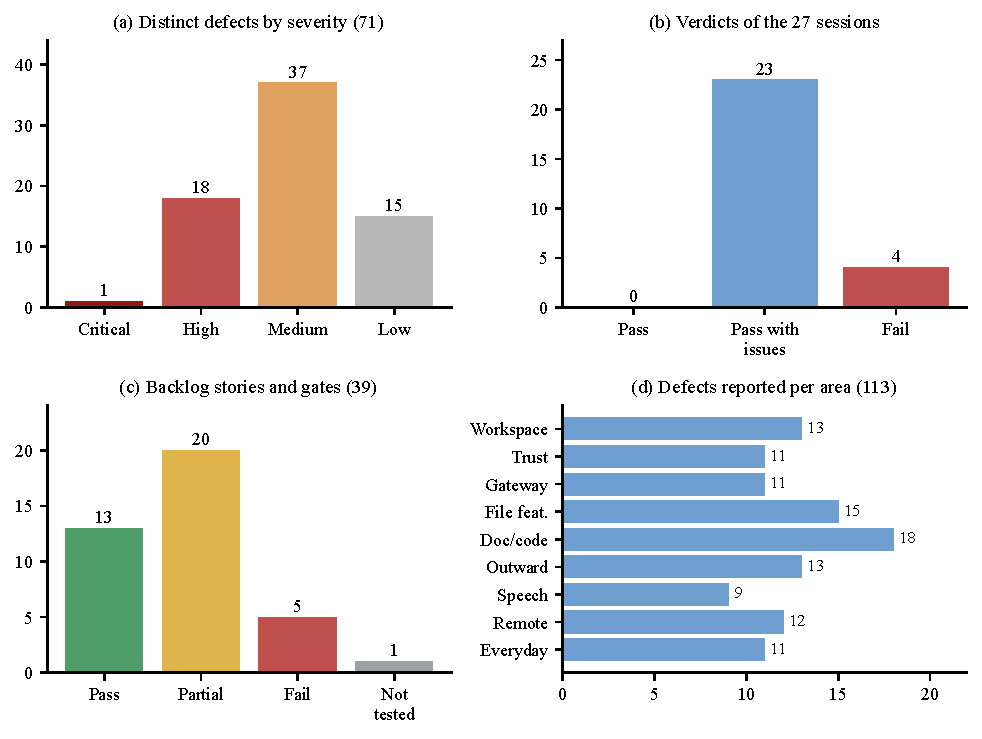
\includegraphics[width=\textwidth]{Figures/fig_campaign.pdf}
    \caption{Results of the interface campaign.}
    \label{fig:campaign}
\end{figure}

\textbf{Results.} Figure~\ref{fig:campaign} summarises the campaign. No session found a clean pass: none of the 27 sessions ended with the verdict pass, 23 ended with pass with issues and 4 with fail (panel b). Of the 39 backlog stories and stage gates, 13 passed, 20 passed in part, 5 failed and one could not be tested (panel c). The sessions reported 113 defects, which merged into 71 distinct defects, being 1 critical, 18 high, 37 medium and 15 low (panel a), together with 63 behaviours that work but that a user would not want. The reports were spread across all nine areas (panel d), with document and code understanding drawing the most (18) and speech input and output the fewest (9).

\textbf{What held.} Across many phrasings the system never deleted anything and refused any attempt to reach outside the chosen folder in plain words. Nothing left the computer, by web search or mail, without an approval card, and double clicks and stale clicks did not run a plan twice. Code questions produced only a difference and never an edit. Voice could not approve, delete or send. A phone could not approve emails or searches, saw only the folders ticked for it, and could be removed instantly. Tidy previewed every step, undo worked in ordinary use, and the rule that automation is offered only after three repetitions was exact.

\textbf{What failed.} The principal defects, with their severity, were the following.
\begin{itemize}
    \item \textbf{Critical.} When a tidy encounters two files with the same destination name, undo will lose one of them, claiming to restore the files as they were. This is the opposite of what it promised that nothing will be lost, although there is no deletion operation, and is the first error that needs to be fixed.
    \item \textbf{High, visibility.} The history of what ARTEMIS did is on disk but not on screen, the page on which changes are reported can tell you that nothing changed when files were transferred, and a banner may remain telling that nothing had been sent since a search.
    \item \textbf{High, boundary.} The microphone might remain live with voice switched off; a plan that a phone had left waiting still executed after its folder was un-shared; a conversation might copy the contents of one folder to another; and any drive, including the system drive, could be added as a folder.
    \item \textbf{High, trustworthy answers.} Some answers provided by the system included no source, said nothing was found when it was in the files, referenced to the incorrect file, or included an email that stated it attached an attachment that was not there. Not all the gates that label unsupported claims fired.
    \item \textbf{Medium and low.} The voice panel would clutter the page, messages would be sent with the system being busy or messages sent before a reload would disappear and new files were not displayed until the user requested the system to look at the changes..
\end{itemize}

\textbf{Discussion.} The trend is educative. The mechanisms that are meant to support the hypothesis, consisting of the single resolution point, the tiers, the dispatcher and the undo journal, withstood adversarial use, and the majority of the severe defects are in how an interface control is wired to a gate, what a screen reports, and in cases the unit tests did not model, such as a name collision or a shared folder with a plan awaiting an allocation. This lends significance to the architectural decision to construct the enforcement first, as well as demonstrates that correctness in isolation of enforcement is not enough to provide the trust that the hypothesis predicts, as many of these defects would ruin trust in practice. Limits. The testers were not individuals but automated agents hence their reports reflect what breaks and not how an individual feels of the same. They were unable to listen to audio, could not confirm the presence of a model of cloud answer or a real email leave, did not test the side of the relay, the seven days of retaining chats or the deleting of the remote plane, and ran on a machine not embedding the model, which likely exaggerates the retrieval failures. Some of the most atrocious results are the results of a single session and these should be noted as such in the consolidated report, therefore they should be re-checked after correction. The work of the second phase is all carried over as 71 defects.

\section{E5: Observations of Prospective Users}
\textbf{Method.} The team members had contact with 30 potential users who were students, developers, human resources employees and non-technical users. The project pitch was used to explain the idea and the participants were able to try the current prototype. They were questioned whether they could trust an assistant that works as ARTEMIS explains and they were at liberty to say what they thought about the idea and the prototype. The responses below are those reported by the team from these conversations.

{\Needspace*{7\baselineskip}
\begin{longtable}{|p{6.4cm}|r|r|}
\caption{Stated trust, 30 prospective users.}\label{tab:obs}\\*
\hline
\textbf{Response} & \textbf{People} & \textbf{Share of 30} \\*
\hline
\endfirsthead
\caption[]{continued from previous page}\\*
\hline
\textbf{Response} & \textbf{People} & \textbf{Share of 30} \\*
\hline
\endhead
\hline
Fully agree they would trust it & 10 & 33\% \\*
\hline
Partly agree they would trust it & 16 & 53\% \\*
\hline
\textbf{Total expressing trust} & \textbf{26} & \textbf{87\%} \\
\hline
Did not express trust & 4 & 13\% \\
\hline
\end{longtable}
}

\begin{figure}[H]
    \centering
    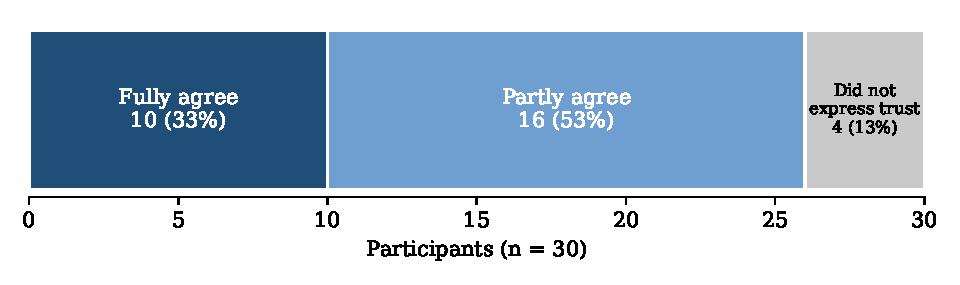
\includegraphics[width=0.92\textwidth]{Figures/fig_obs_trust.pdf}
    \caption{Stated trust among 30 prospective users.}
    \label{fig:obs}
\end{figure}

\textbf{Results.} In general, the general concept was quite acceptable in all the four backgrounds. Twenty-six of 30 indicated trust, 10 of them entirely and the partial assent was always conditional: participants were ready to trust the assistant on the condition that it does what it claims. The participants who tested the application stated that it was a prototype of the application as it was. They dissociated this judgement and the concept and they claimed that they would be happy to embrace the end product as stipulated in the pitch.

\textbf{Discussion.} The status of participants which is bound to their trust is the status of the architecture being constructed to fulfil, as the trustworthiness of the assistant is supposed to be based on the boundary and on the steps in approval acting as it is promised and not on its good motives. It is also 108 the circumstance that the faults of the last part endanger, or, in other words, that the promise made is accompanied by the good effect, as well as by the labour that is left. The finding is similar to the underlying questionnaire where 65 percent of 374 participants found an assistant based on a workspace as more trustworthy than one based on full access, but the two questions are different, and the numbers should not be summed. Limits. The participants consist of 30 individuals who were contacted via the personal connections of the team and are not representative sample. The team collected responses in a conversation and summarised them, thus there is no data on individual responses or recordings. The answers were not counted by background and thus no figure is claimed to any of the groups. The reasons of the four participants who did not express trust were not recorded. The measures of the stated attitudes are post-pitch and short trial responses and not sustained use. They should be interpreted as pointing evidence..

\section{E6: Exploratory Persona Simulation}
\textbf{Method.} To test the idea under sceptical review and to expose objections that friendly conversation might not, 15 simulated personas, including students, developers, a freelancer, employees and deliberately sceptical non-adopters, were given a neutral description of the idea and a private copy of the prototype, and each reported its first impressions, what it did, its ratings and its objections in a structured report. Each worked independently and the agents did not see each other's reports. The study uses language-model-based simulated user agents to explore potential user perceptions and behavioural patterns. The participants are simulated personas and not recruited human subjects, so the results are exploratory synthetic evidence and must not be presented as empirical human-subject findings or as statistically representative of any population. They are reported here only as a stress test of the argument.

{\Needspace*{3\baselineskip}
\begin{longtable}{|p{8.0cm}|p{5.2cm}|}
\caption{Persona simulation results.}\label{tab:sim}\\*
\hline
\textbf{Question} & \textbf{Result} \\*
\hline
\endfirsthead
\caption[]{continued from previous page}\\*
\hline
\textbf{Question} & \textbf{Result} \\*
\hline
\endhead
\hline
Would an assistant limited to chosen folders be trusted more than one with full access? & 6 agree, 9 partly, 0 disagree \\*
\hline
Would that make them more willing to use it? & 1 agree, 14 partly, 0 disagree \\*
\hline
Does the limitation cost too much usefulness? & 6 no, 3 partly, 6 cannot say, 0 yes \\
\hline
Is wanting broad access a barrier for them? & 10 agree, 2 partly, 3 disagree \\
\hline
Would they accept one mistake if undo is easy? & 7 agree, 8 partly, 0 disagree \\
\hline
Ask before every change, or act and let me undo? & 8 ask first, 6 mixed, 1 act then undo \\
\hline
Perceived relevance of the problem (1 to 5) & Mean 3.27, median 3 \\
\hline
Perceived value of the solution (1 to 5) & Mean 2.8, median 3 \\
\hline
Adoption & 14 might try, 1 would not use, 0 would use or recommend \\
\hline
\end{longtable}
}

\textbf{Discussion.} The simulation is more reserved than the observations of real people, and that is its use. No persona disagreed that bounding scope would raise trust, which agrees in direction with E5, but only 1 of 15 would be clearly more willing to use it, and most attached conditions. Concerns were raised by all 15: 13 described failed, wrong or partial answers, and 12 noticed that a cloud key appeared as already saved in a clean copy, which could not be resolved as a defect or as an artefact of the shared test machine. Approval fatigue and long-term retention cannot be observed in a single session and were not. Limits. The personas are played by one underlying model, so their views are not independent, and such agents can be agreeable. The sample is small, no statistical test is used, and defects of the prototype, notably the failures of the folder box, probably coloured the personas' reactions. The results are therefore a check on the reasoning and are not evidence of adoption.

\section{Discussion}
\subsection{Findings against the Central Hypothesis}
Table~\ref{tab:hyp} sets the evidence against the three parts of the central hypothesis. The classification is a description of the weight of the first-phase evidence and not a statistical test.

{\Needspace*{7\baselineskip}
\begin{longtable}{|p{3.0cm}|p{7.2cm}|p{2.9cm}|}
\caption{Assessment of the central hypothesis.}\label{tab:hyp}\\*
\hline
\textbf{Part} & \textbf{Evidence} & \textbf{Assessment} \\*
\hline
\endfirsthead
\caption[]{continued from previous page}\\*
\hline
\textbf{Part} & \textbf{Evidence} & \textbf{Assessment} \\*
\hline
\endhead
\hline
Restricting scope increases trust & Questionnaire (65 percent of 374); E5 (26 of 30, 10 fully); E6 (6 agree, 9 partly, none disagree); E4 shows the boundary mechanisms hold under hostile use & Supported in direction; conditional on exact behaviour \\*
\hline
Increases willingness to adopt & E5: willingness to adopt the final product as pitched; E6: 14 might try, 1 clearly more willing & Partly supported; rests on stated intention \\*
\hline
Without meaningfully reducing usefulness & E4 and E6 show the limits were not what users objected to; no task measure exists yet & Not yet tested \\
\hline
\end{longtable}
}

Not yet tested meaningfully users objected to; no task measure exists yet reducing usefulness On this evidence the first part is supported in direction and the second is partly supported, and the third cannot be determined until usefulness is determined on the tasks. The entire hypothesis is hence promoted by the initial stage and is not confirmed yet. With the stricter interpretation of the simulation, where the only agreement that matters is the clear one, the adoption part would not support the study, and this is one of the reasons why the second phase with the controlled study should be the most weighty.

\subsection{Findings against the Research Question}
The research question is: Does an assistant confined to given workspaces manage to provide viable multi-step task automation and enhance trust without diminishing usefulness? The prototype demonstrates that the restriction can be constructed as structure rather than policy, and can be constructed inexpensively, introducing less than a millisecond to a call. It demonstrates that, multi step plans, tidying, cited answers, mail, search, drafting, voice and remote control can be executed on the same three points of enforcement. It does not yet demonstrate that the automation is user-friendly, since that requires the task study, and the flaws of E4 indicate that reliability, and not the limitation, is what is presently limiting the experience.

\subsection{Threats to Validity}
There are four types of evidence with their respective weaknesses. The deterministic tests are unable to work out a real model. The interface campaign employed automated agents that are not able to hear or feel and one of the machines had no embedding model. The team collected the observations of 30 people, constructed the system and introduced it, which may favourably respond, and was not recorded in the individual scores. The simulation is synthetic. All these weaknesses are in different directions hence the four are reported separately and not brought together and none of them is presented as the controlled study that the second phase will offer.

\subsection{Evaluation Not Yet Done}
111 The subsequent components of the evaluation process of Chapter 5 have not been conducted and are scheduled to be implemented during the second phase: task-based measurements with the system and without it, the subjective workload measure, the usability and trust questionnaires, approval fatigue with repeated sessions, measuring the synthesis faithfulness and citation accuracy with an actual model, and the voice measure with the four-second latency target.

\section{Conclusion}
The initial stage demonstrates that the enforcement the hypothesis is based on is constructable, is run at insignificant cost and survives under adversarial use, and that potential users as questioned responded to the concept with confidence conditional on the system doing just what it says. It also demonstrates that the prototype does not yet necessarily do what it claims: the interface campaign represented 71 various defects, one of them a critical one, and the difference between a passing automated suite and a working interface was huge. The evidence validates the hypothesis direction and its aspect of trust, partially supports adoption, and measures usefulness remains to be quantified. The corrections of the defects found and the controlled study are the two main tasks of the second phase.

\chapter{Conclusions}
\section{Summary of the Work Done}
The project aimed to demonstrate that an assistant limited to folders that the user explicitly gives, and asks before it performs and can undo whatever it did, can be trusted and used with little loss of utility to an assistant with complete access. The initial stage defined the problem and the hypothesis with a questionnaire of 374 respondents and 13 interviews, consulted 26 studies in seven themes, defined the requirements, and created an architecture which transforms the hypothesis into three enforcement points: a workspace broker which alone resolves paths, a policy engine which places every action in one tier, and a dispatcher which alone acts. It then developed a functioning prototype of some 14,250 lines in eight steps, including the workspace base, an optional remote plane, and tested it with 554 automated tests and two hand-on rounds, a 27-session interface campaign, and interviews with 30 potential users.

\section{Findings and Results}
The enforcement layer is also designed to perform as advertised and withstands adversarial usage. No deletions or accesses were made to any file during a session, no files outside the selected folder were accessible, and no files left the computer without approval, and these properties took less than a milliseconds per call. The idea was met with conditional trust by the prospective users with 26 of 30 indicating that they trusted it and 10 of them said they would embrace the end product as it was being pitched. The prototype itself is not ready for users. The interface campaign discovered 71 different bugs, one of which is a critical bug where undo following a name collision may lose a file, and demonstrated that a passing automated test can have a significantly broken interface. Responses to questions on files were occasionally not supported or incorrect, and the history on what the assistant had done was not clearly visible..

\section{Coverage of the Scope and Objectives}
Table~\ref{tab:objectives} states, for each objective of Chapter 2, whether it has been met.

{\small
\Needspace*{3\baselineskip}
\begin{longtable}{|p{4.6cm}|p{2.3cm}|p{7.3cm}|}
\caption{Status of the project objectives.}\label{tab:objectives}\\*
\hline
\textbf{Objective} & \textbf{Status} & \textbf{Basis and remaining work} \\*
\hline
\endfirsthead
\caption[]{continued from previous page}\\*
\hline
\textbf{Objective} & \textbf{Status} & \textbf{Basis and remaining work} \\*
\hline
\endhead
\hline
Operate strictly within granted folders & Largely met & Boundary holds in all tests; any drive can still be added, a chat can carry one folder's content to another, and a waiting remote plan outlived an un-shared folder. \\*
\hline
Reduce time spent on resumption and routine file work & Not yet measured & Needs the task study of the second phase. \\*
\hline
Keep the user in control through preview, approval and undo & Largely met & Gates hold; undo can lose a file on a name collision. \\
\hline
Provide no code path to deletion & Met & No deletion operation exists and none was reachable in any session. \\
\hline
Make everything held visible and deletable & Partly met & The panel works; the activity record is not fully visible. \\
\hline
Support voice under the same gates & Met for gates & No new gate was needed; microphone control and recognition quality need work. \\
\hline
Evaluate on time, workload, usability and trust & Not yet done & Planned for the second phase. \\
\hline
\end{longtable}
}

The functional scope of Chapter 2 was covered in full as a prototype: every capability listed there exists and runs through the gates, including the optional remote plane. The scope was not covered in the sense of readiness, because several capabilities are unreliable, and two of the four deliverables are not yet complete, being the user manual, which will be written once the interface has stabilised, and the evaluation report, which depends on the study of the second phase.

\section{Challenges Faced}
Four challenges shaped the first phase. The first was the gap between component tests and a working interface. The first hands-on round found that nearly every feature was unreachable although all unit tests passed, and the interface campaign later found 71 defects, which taught that the interface must be tested as a whole and that each defect needs a regression test. The second was the nondeterminism of a small local model, which sometimes gave unsupported or wrong answers, and which the gates mitigate but cannot cure. The third was the constraints of the interface framework, which required hidden controls to be triggered by scripts for some interactions and made voice behaviour, such as repeated speech, speaking the model's label, and losing the thread of a conversation, difficult to get right, and these were corrected in turn. The fourth was the size of the task for a team of three in one semester, which required the highest-risk components to be built first and the evaluation to be deferred.

\section{What Has Been Left Out and Why}
The controlled evaluation, the user manual, the measurement of approval fatigue and the quality evaluation of synthesis and citations are left to the second phase, because each depends on a stable interface. Real audio, a cloud model answer, a real email and the relay's own side were not exercised in the interface campaign, because the testing agents could not hear, did not hold credentials and must not use real accounts. The 71 defects are known and recorded and have not yet been fixed.

\section{Recommendations and Future Work}
The first recommendation is to correct, before anything else, the defects that bear directly on the promises the system makes: make tidy and undo collision-safe so that a file is never overwritten and any step that cannot be restored is reported; refuse drive roots and system folders when adding a folder; stop the microphone completely when voice is off; recheck the folder grant when a waiting plan is approved from a phone; stop a chat from carrying one folder's content into another; and make the activity record and the page that reports changes truthful. The second is to make answers honest, so that an answer with no source is plainly labelled, a missing embedding model is detected and reported, and retrieval failures that say not found for facts that are present are removed. The third is to add a regression test for every defect found at the interface, and to run the interface scenarios of the campaign as part of the suite. The fourth is to carry out the controlled study of Chapter 5. Beyond the second phase, directions worth pursuing are configurable approval granularity, since the questionnaire found users evenly divided, onboarding that takes minutes and not tens of minutes, barge-in and lower latency in voice, and a check that a citation actually supports its claim and not only that it exists.

\section{Plan for FYP-II}
The second phase has about sixteen weeks. The plan in Table~\ref{tab:plan} orders the work so that the product is stable before it is evaluated, since a study of a prototype that is still changing would measure the changes and not the idea.

The principal risks to this plan are recruitment, which depends on the institution's networks as the risk analysis of Chapter 4 notes, and the possibility that correcting defects takes longer than allowed. The mitigation is that the order of work places stability first, so that if the study must be smaller it can be reduced in size without being run on an unstable product, and that the defect work is limited to those defects that bear directly on the project's promises.

{\small
\Needspace*{10\baselineskip}
\begin{longtable}{|p{1.4cm}|p{7.0cm}|p{5.8cm}|}
\caption{Plan of work for the second phase.}\label{tab:plan}\\*
\hline
\textbf{Weeks} & \textbf{Work} & \textbf{Deliverable and exit check} \\*
\hline
\endfirsthead
\caption[]{continued from previous page}\\*
\hline
\textbf{Weeks} & \textbf{Work} & \textbf{Deliverable and exit check} \\*
\hline
\endhead
\hline
1 to 2 & Correct the defects that bear on the promises: collision-safe tidy and undo, drive and system folder refusal, microphone control, remote grant recheck, cross-folder chat memory. Add a regression test for each. & All critical and high defects of the boundary and recovery groups closed; the suite grows by the regression tests. \\*
\hline
3 to 4 & Honest answers and visibility: label unsupported answers, detect and report a missing embedding model, repair false not-found answers, show a readable activity view and a live record of what left the computer. & Re-run of the campaign scenarios for these groups shows no repeat of the defects. \\*
\hline
5 to 6 & Onboarding and interface: guard-rails and background indexing in the folder box, voice panel layout, no silently lost messages, visibility of new files. Voice latency and barge-in. & Medium defects of the interface group closed; time for a new user to reach a first answer measured. \\
\hline
7 & Re-run of the full interface campaign, including the remote plane's relay side, retention of chats and removal of the remote plane. & Updated defect register; stage gates that were not tested are now tested. \\
\hline
8 & User manual (Chapter 8). & Complete manual written from the stabilised interface. \\
\hline
9 to 10 & Design the controlled study: tasks, instruments for workload, usability and trust, consent and ethics approval, recruitment through the institution. Pilot with a small group. & Study protocol approved by the supervisor; pilot completed and the instruments revised. \\
\hline
11 to 13 & Conduct the study: task completion with and without the system, repeated sessions for approval fatigue, measurement of synthesis faithfulness and citation accuracy, voice latency against the four-second target. & Data collected for the planned number of participants. \\
\hline
14 & Analyse the results and classify the central hypothesis and each supporting claim against the criteria fixed beforehand. & Analysis tables and figures. \\
\hline
15 & Complete the report: full Chapter 9, final Chapter 10, updated manual. & Final report draft to the supervisor. \\
\hline
16 & Final fixes, demonstration preparation and defence. & Demonstration build and final submission. \\
\hline
\end{longtable}
}

\section{Conclusion of the Report}
The initial step has yielded a prototype where the key concept, that the area of an assistant can be restricted by design and its actions can be reviewed and undone at low cost, has been put into practice and is tested under hostile conditions at negligible cost, and potential users who were consulted have responded with confidence that relied on the system doing precisely what it claims to. The same phase revealed that the prototype is yet to do so everywhere, and the defects are documented. It is only left to ensure that the product is reliable and measure, among the participants and in tasks, whether the trust earned is worth an acceptable cost in utility. The second phase is that..


{
\bibliographystyle{ieeetr}
\bibliography{fypbib}
}

\appendix
\chapter{Research Instruments and Response Distributions}
This appendix records the instruments used in the foundational research and the complete response distributions summarised in Chapters 2 and 3. It is included so that the findings cited throughout the report can be examined at the level of the underlying data.

\section{Research Method}
The foundational research comprised two instruments. A questionnaire of seventeen items drew 374 valid responses, covering the respondent's context, the problem, design and trust preferences, and feature demand, with attitudinal items using a five-point scale. An interview guide coded thirteen in- person conversations on five axes: the last occasion on which the participant lost their place in multi- file work, the workaround they already employ, their reaction to the concept, the effect a trust- breaking mistake would have, and whether they would continue using the system.

Recruitment was through the institution's student and practitioner networks, and the questionnaire ran from 22 to 27 August 2026. Four limitations apply and are stated because they bound every conclusion drawn from this data. The sample is self-selected and drawn from a single institution. Students predominate, so the professional signal rests on a smaller subsample. The system was described in text rather than demonstrated, so predicted use and predicted churn are stated intentions rather than observed behaviour. Some free-text responses contain near-identical phrasings, which suggests that certain answers were presented as suggested text, so theme counts should be read as indicative.

\section{Respondent Profile}
Table~\ref{tab:appprofile} gives the composition of the sample and the frequency with which respondents perform multifile work.

{\Needspace*{7\baselineskip}
\begin{longtable}{|p{6.0cm}|r|r|}
\caption{Respondent role and work frequency.}\label{tab:appprofile}\\*
\hline
\textbf{Response} & \textbf{Count} & \textbf{Percent} \\*
\hline
\endfirsthead
\caption[]{continued from previous page}\\*
\hline
\textbf{Response} & \textbf{Count} & \textbf{Percent} \\*
\hline
\endhead
\hline
\multicolumn{3}{|l|}{\textbf{Role}} \\
\hline
Student & 302 & 80.7 \\
\hline
Developer or software engineer & 47 & 12.6 \\
\hline
Freelance & 12 & 3.2 \\
\hline
Employed & 7 & 1.9 \\
\hline
Other & 6 & 1.6 \\
\hline
\multicolumn{3}{|l|}{\textbf{Frequency of multi-file project work}} \\
\hline
Daily & 147 & 39.3 \\
\hline
A few times a week & 159 & 42.5 \\
\hline
A few times a month & 68 & 18.2 \\
\hline
\multicolumn{3}{|l|}{\textbf{Prior use of an AI assistant}} \\
\hline
Yes, regularly & 172 & 46.0 \\
\hline
Yes, occasionally & 115 & 30.7 \\
\hline
Tried once or twice & 48 & 12.8 \\
\hline
Never & 39 & 10.4 \\
\hline
\end{longtable}
}

\section{Headline Findings}
The nine findings established by the research, referenced throughout Chapters 2 and 4, are as follows.

\begin{itemize}
    \item \textbf{F1.} The reorientation problem is real. 44 percent of respondents struggle to recall what they were doing on returning to a project after a break, and only 7 percent never do
    \item \textbf{F2.} File disorder outpaces manual cleanup for 59 percent of respondents
    \item \textbf{F3.} The problem costs real time at moderate scale, with 42 percent losing more than an hour a week and 14 percent more than three hours
    \item \textbf{F4.} The work is unautomated because of distrust of automation at 36 percent and lack of knowhow at 28 percent, rather than because the tasks do not exist
    \item \textbf{F5.} The bounded-workspace hypothesis holds. 65 percent rate a workspace-only assistant more trustworthy than a full-access one, with a mean of 3.8, and 40 percent prefer local-first operation
    \item \textbf{F6.} Users are forgiving of a single mistake. 65 percent would continue using the system after one wrong suggestion and only 10 percent would abandon it
    \item \textbf{F7.} The principal retention risks are habit fit at 27 percent and an untrusted mistake at 24 percent; approval fatigue is real but smaller at 10 percent
    \item \textbf{F8.} Feature demand is concentrated on session resume, notes synthesis and folder tidy, with speech last by a wide margin
    \item \textbf{F9.} The interviews confirm the questionnaire and add effortless onboarding as a named condition for continued use
\end{itemize}

\section{Segment Analysis}
Table~\ref{tab:appsegments} presents selected measures by respondent segment. Role does not predict the interaction preference, since students and developers give near-identical workspace-trust ratings and identical approvalfirst shares. Experience moves it modestly: regular users of assistants prefer approval-first less often than light or non-users, which is consistent with heavier users being more comfortable delegating. The effect is small and neither group approaches unanimity, so the practical conclusion is unchanged, which is that the interaction model must be a setting rather than a fixed decision.

{\Needspace*{7\baselineskip}
\begin{longtable}{|p{5.2cm}|r|p{2.4cm}|p{2.2cm}|p{2.0cm}|}
\caption{Selected measures by respondent segment.}\label{tab:appsegments}\\*
\hline
\textbf{Segment} & \textbf{n} & \textbf{Workspace trust (mean)} & \textbf{Prefer approval-first} & \textbf{Prefer local-first} \\*
\hline
\endfirsthead
\caption[]{continued from previous page}\\*
\hline
\textbf{Segment} & \textbf{n} & \textbf{Workspace trust (mean)} & \textbf{Prefer approval-first} & \textbf{Prefer local-first} \\*
\hline
\endhead
\hline
All respondents & 374 & 3.8 & 51\% & 40\% \\
\hline
Students & 302 & 3.8 & 51\% & 41\% \\
\hline
Developers and engineers & 47 & 3.7 & 51\% & 36\% \\
\hline
Regular assistant users & 172 & 3.9 & 44\% & 40\% \\
\hline
Light or non-users & 87 & 3.8 & 59\% & 41\% \\
\hline
\end{longtable}
}

\section{Interview Findings}
Figure~\ref{fig:interview} presents the coded interview responses. Ten of the thirteen participants reacted positively to the concept, with the remainder split between conditional, mixed and one negative response. Eight of thirteen said a single mistake would not stop them, several qualifying this with caution, while two said a trust-breaking mistake would cause them to stop. Six said outright that they would continue using the system and four said they would do so conditionally, with effortless onboarding named as the most common condition, followed by privacy and by the system reaching sufficient maturity.

\begin{figure}[H]
    \centering
    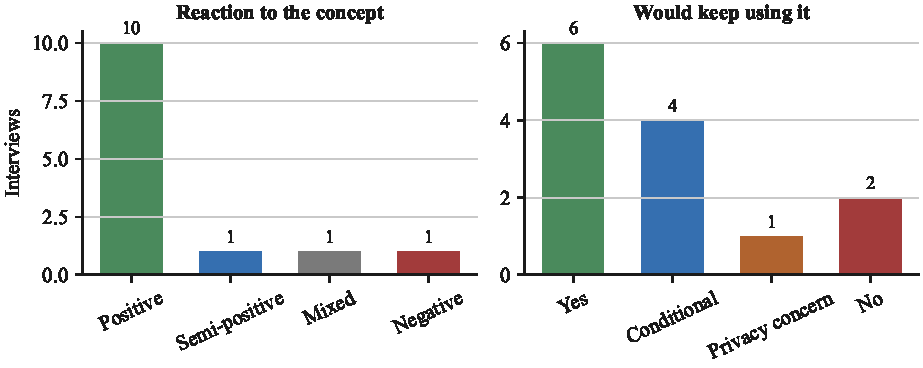
\includegraphics[width=\textwidth]{Figures/fig_interview.pdf}
    \caption{Coded interview responses (13 interviews).}
    \label{fig:interview}
\end{figure}

The workarounds participants already employ were consistent: informal notes written by hand or with an assistant to record where they left off, repeated manual restructuring because every project has a different structure, and simply tolerating the friction because automating it appears to cost more than it saves.

\section{Additional Response Distributions}
Figures~\ref{fig:messy}, \ref{fig:wstrust}, \ref{fig:localcloud}, \ref{fig:mistake}, \ref{fig:likely}, \ref{fig:churn} and \ref{fig:themes} present the remaining distributions underlying the findings cited in Chapters 2 and 4.

\begin{figure}[H]
    \centering
    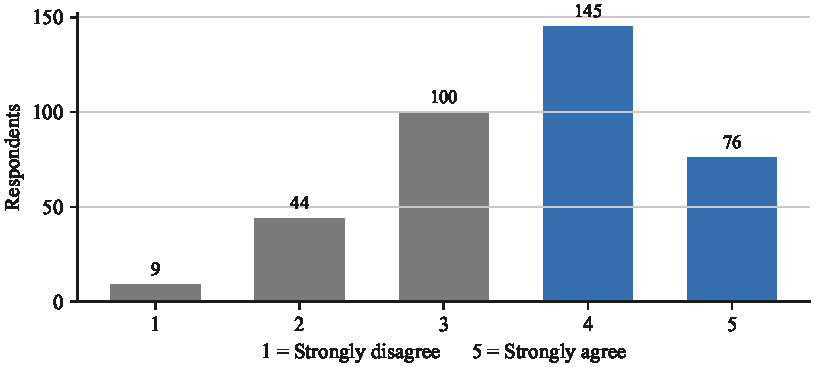
\includegraphics[width=0.82\textwidth]{Figures/fig_messy_agree.pdf}
    \caption{Agreement that files become disorganised.}
    \label{fig:messy}
\end{figure}

\begin{figure}[H]
    \centering
    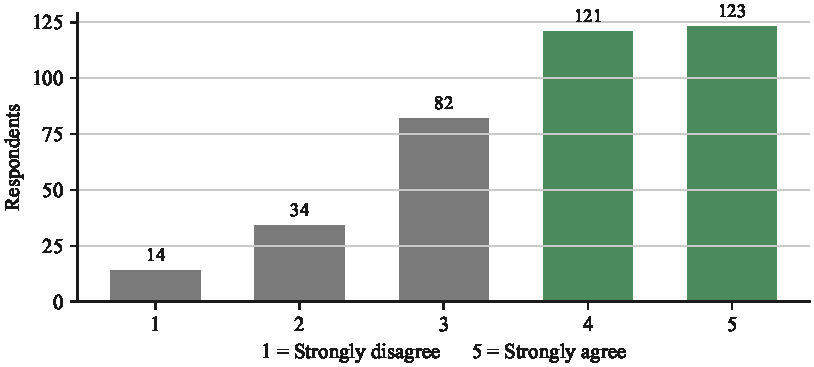
\includegraphics[width=0.82\textwidth]{Figures/fig_workspace_trust.pdf}
    \caption{Agreement on workspace-only trust.}
    \label{fig:wstrust}
\end{figure}

\begin{figure}[H]
    \centering
    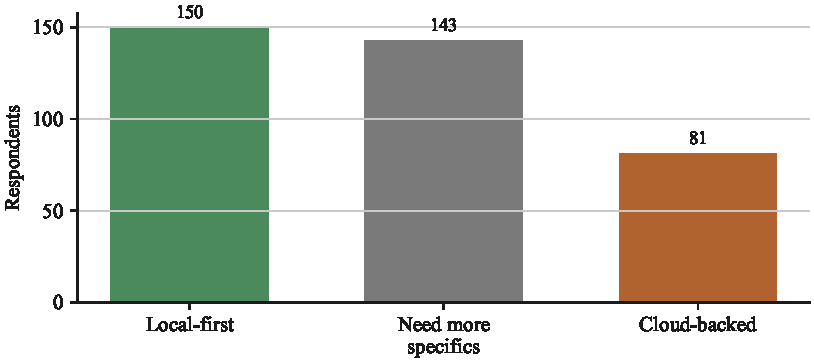
\includegraphics[width=0.82\textwidth]{Figures/fig_local_vs_cloud.pdf}
    \caption{Local versus cloud preference.}
    \label{fig:localcloud}
\end{figure}

\begin{figure}[H]
    \centering
    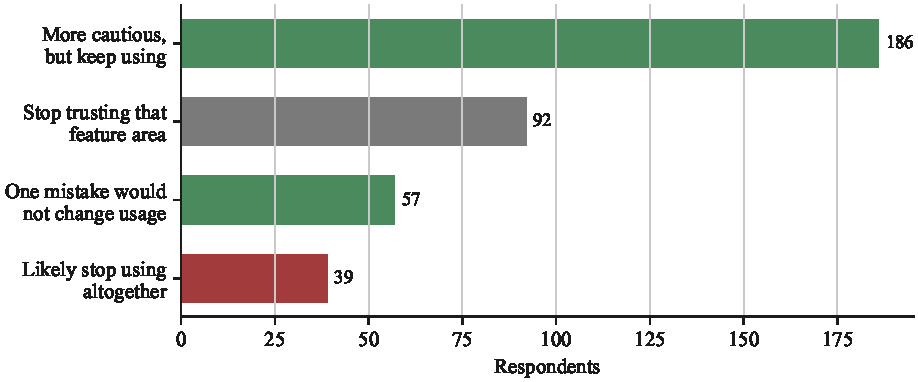
\includegraphics[width=\textwidth]{Figures/fig_wrong_suggestion.pdf}
    \caption{Response to a single wrong or unwanted suggestion.}
    \label{fig:mistake}
\end{figure}

\begin{figure}[H]
    \centering
    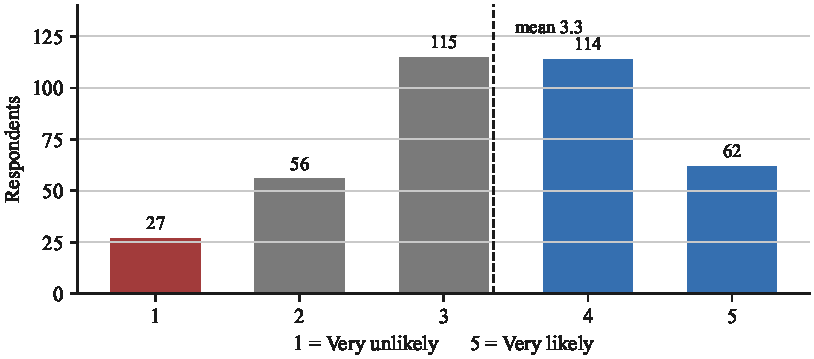
\includegraphics[width=0.82\textwidth]{Figures/fig_likely_use.pdf}
    \caption{Likelihood of continued use after the novelty.}
    \label{fig:likely}
\end{figure}

\begin{figure}[H]
    \centering
    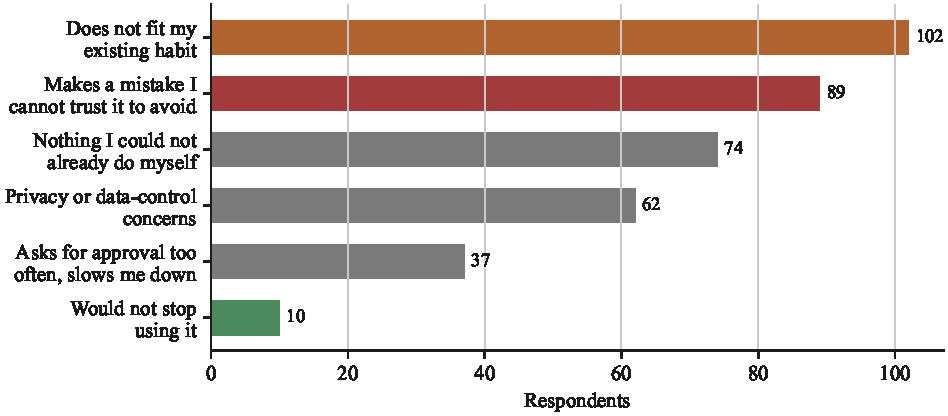
\includegraphics[width=\textwidth]{Figures/fig_stop_reason.pdf}
    \caption{Most likely reason for stopping after a week.}
    \label{fig:churn}
\end{figure}

\begin{figure}[H]
    \centering
    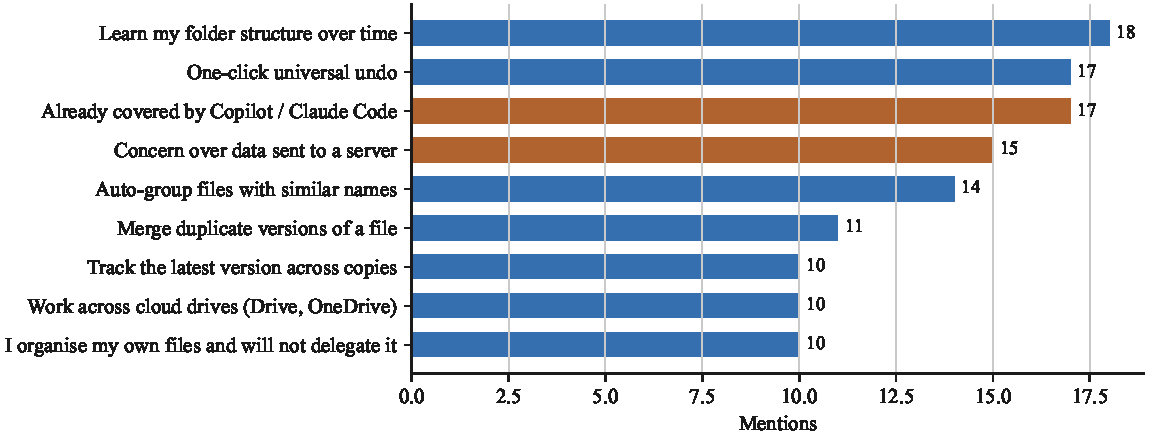
\includegraphics[width=\textwidth]{Figures/fig_open_feedback_themes.pdf}
    \caption{Recurring themes in free-text responses.}
    \label{fig:themes}
\end{figure}

\end{document}
